% !TeX program = xelatex
% =====================================================================
%  Witten, "A New Look At The Path Integral Of Quantum Mechanics"
%  arXiv:1009.6032v1 — 中文译注本
%  编译：xelatex（推荐 latexmk -xelatex），需 ctex 宏包
% =====================================================================
\documentclass[11pt,a4paper,UTF8]{ctexart}

% ---------- 页面与版式 ----------
\usepackage[a4paper,left=2.6cm,right=2.6cm,top=2.6cm,bottom=2.8cm]{geometry}
\usepackage{fancyhdr}
\pagestyle{fancy}
\fancyhf{}
\fancyhead[L]{\small\itshape A New Look At The Path Integral Of Quantum Mechanics}
\fancyhead[R]{\small\thepage}
\renewcommand{\headrulewidth}{0.4pt}

% ---------- 数学 ----------
\usepackage{amsmath}
\usepackage{amssymb}
\usepackage{amsthm}
\usepackage{mathtools}
\usepackage{bm}

% ---------- 图形、颜色、表格、列表 ----------
\usepackage{graphicx}

\usepackage{xcolor}
\usepackage{booktabs}
\usepackage{array}
\usepackage{enumitem}
\usepackage{caption}
\captionsetup{font=small,labelsep=quad}
% 允许极少量额外伸展，避免中文+长公式造成的 overfull
\setlength{\emergencystretch}{3em}

% ---------- 超链接 ----------
\usepackage[colorlinks=true,linkcolor=blue!55!black,citecolor=blue!55!black,
            urlcolor=blue!55!black,unicode]{hyperref}

% ---------- 定理类环境 ----------
\theoremstyle{plain}
\newtheorem{theorem}{定理}[section]
\newtheorem{proposition}[theorem]{命题}
\newtheorem{lemma}[theorem]{引理}
\newtheorem{corollary}[theorem]{推论}
\theoremstyle{definition}
\newtheorem{definition}[theorem]{定义}
\newtheorem{remark}[theorem]{注}
\renewcommand{\proofname}{证明}

% ---------- 每节重点（Key Takeaways） ----------
\newenvironment{keypoints}{%
  \par\addvspace{0.9em}%
  \noindent\begin{minipage}{\linewidth}%
  \color{black!80}\rule{\linewidth}{0.6pt}\par\vspace{2pt}%
  \noindent\textbf{【本节重点】}\par\vspace{2pt}%
  \begin{itemize}[leftmargin=1.6em,itemsep=1pt,topsep=2pt,parsep=0pt]%
}{%
  \end{itemize}\vspace{1pt}\noindent\color{black!80}\rule{\linewidth}{0.6pt}%
  \end{minipage}\par\addvspace{0.9em}%
}

% ---------- 常用记号 ----------
\newcommand{\R}{\mathbb{R}}
\newcommand{\C}{\mathbb{C}}
\newcommand{\Z}{\mathbb{Z}}
\newcommand{\dd}{\mathrm{d}}
\newcommand{\ee}{\mathrm{e}}
\newcommand{\ii}{\mathrm{i}}
\newcommand{\Tr}{\operatorname{Tr}}
\newcommand{\tr}{\operatorname{tr}}
\renewcommand{\Re}{\operatorname{Re}}
\renewcommand{\Im}{\operatorname{Im}}
\newcommand{\sgn}{\operatorname{sgn}}
\newcommand{\diag}{\operatorname{diag}}
\newcommand{\id}{\mathrm{id}}
\newcommand{\Hh}{\mathcal{H}}
\newcommand{\Mm}{\mathcal{M}}
\newcommand{\Nn}{\mathcal{N}}
\newcommand{\Oo}{\mathcal{O}}
\newcommand{\Aa}{\mathcal{A}}
\newcommand{\Bb}{\mathcal{B}}
\newcommand{\Cc}{\mathcal{C}}
\newcommand{\Dd}{\mathcal{D}}
\newcommand{\Ee}{\mathcal{E}}
\newcommand{\Ff}{\mathcal{F}}
\newcommand{\Gg}{\mathcal{G}}
\newcommand{\Ii}{\mathcal{I}}
\newcommand{\Jj}{\mathcal{J}}
\newcommand{\Kk}{\mathcal{K}}
\newcommand{\Ll}{\mathcal{L}}
\newcommand{\Pp}{\mathcal{P}}
\newcommand{\Qq}{\mathcal{Q}}
\newcommand{\Ss}{\mathcal{S}}
\newcommand{\Tt}{\mathcal{T}}
\newcommand{\Uu}{\mathcal{U}}
\newcommand{\Vv}{\mathcal{V}}
\newcommand{\Ww}{\mathcal{W}}
\newcommand{\Xx}{\mathcal{X}}
\newcommand{\Yy}{\mathcal{Y}}
\newcommand{\Zz}{\mathcal{Z}}
\newcommand{\fg}{\mathfrak{g}}
\newcommand{\fh}{\mathfrak{h}}

% 标题中的 σ（同时给出 PDF 书签用的纯文本）
\newcommand{\sigmatxt}{$\sigma$}
\pdfstringdefDisableCommands{\def\sigmatxt{σ}}

% =====================================================================
%  前置部分：标题、摘要、译者说明、目录
%  （由 main.tex 以 \input{front} 引入；编译请用 xelatex）
% =====================================================================
\begin{document}
\sloppy

\begin{center}
  {\LARGE\bfseries 量子力学路径积分的新视角}\\[8pt]
  {\large\itshape A New Look At The Path Integral Of Quantum Mechanics}\\[20pt]
  {\large Edward Witten}\\[8pt]
  {\small School of Natural Sciences, Institute for Advanced Study\\
   Einstein Drive, Princeton, NJ 08540 USA\\
   与\\
   Department of Physics, Stanford University, Palo Alto, CA 94305}\\[16pt]
  {\small arXiv:1009.6032v1 [hep-th]，2010 年 9 月 30 日\\[2pt]
   中文译注本}
\end{center}
\vspace{6pt}
\hypersetup{pdftitle={量子力学路径积分的新视角（A New Look At The Path Integral Of
  Quantum Mechanics）},pdfauthor={Edward Witten; 中文译注}}

\begin{abstract}
\noindent
本文将普通量子力学的费曼路径积分复化，并证明：这一复化积分的可能积分围道，与二维
A-模型中的膜（brane）相关联。这为 A-模型与量子力学之间的关系提供了一个相当直接的
解释；过去若干年中，人们已从多种视角研究过这一关系。这些现象在三维陈--西蒙斯
（Chern--Simons）规范理论中有其类比：该理论路径积分中的积分围道，可以由四维
$\mathcal{N}=4$ 超杨--米尔斯（super Yang--Mills）理论导出。因此，在一定条件下，
三维的陈--西蒙斯路径积分等价于四维的 $\mathcal{N}=4$ 路径积分。
\end{abstract}

\section*{译者说明}
\addcontentsline{toc}{section}{译者说明}

\begin{itemize}[leftmargin=1.6em,itemsep=2pt]
  \item \textbf{底本.} 本译文依据 Edward Witten 的 \emph{A New Look At The Path Integral
        Of Quantum Mechanics}（arXiv:1009.6032v1 [hep-th]，77 页）逐页翻译。原书印刷页码
        与本译本的章节、公式编号一一对应。
  \item \textbf{公式编号.} 全部沿用原文编号（如式 (2.37)、式 (A.9)），采用 \verb|\tag{}|
        手工标注，正文中按“式 (2.37)”的形式引用，便于与英文本对照。
  \item \textbf{审校批注.} 以 \verb|% [Tutor Note: ...]| 形式的 \LaTeX{} 注释插入源码
        （编译后不显示），内容包括：符号约定与指标易错处、作者省略证明之处、
        原文印刷笔误。建议对照源码阅读。
  \item \textbf{图表.} 原文图表已从 PDF 中逐一裁出，置于 \verb|figures/| 目录，
        并以 \verb|figure| 环境插入对应段落；图注译为中文并标注原文位置。
  \item \textbf{编译.} 请使用 \texttt{XeLaTeX}（或 \verb|latexmk -xelatex|）编译两遍；
        中文排版依赖 \verb|ctex| 宏包，需本机装有中文字体（Windows/macOS 下自动选用系统字体）。
  \item \textbf{术语.} 译名以国内理论物理界通行译法为准，术语对照表见随附
        \verb|README.md|。
\end{itemize}

\tableofcontents
\newpage


% ===== 片段：sections/s01.tex =====

% =====================================================================
%  §1  引言（原文 pp.3–5，PDF 页 4–7 顶部）
% =====================================================================
\section{引言}
\label{sec:intro}

\begin{keypoints}
  \item \textbf{物理图像：} 洛伦兹号差下的费曼路径积分 $\int\mathcal{D}\Phi\,\ee^{\ii I(\Phi)}$
        可以像普通有限维积分那样解析延拓到复场空间，并改沿复化空间中的“积分围道”来积分；
        不同围道给出同一微分方程（Ward 恒等式）的不同解，因而可能对应不同的量子系统。
  \item \textbf{核心新意：} 对量子力学的相空间路径积分，若把围道取为\textbf{伪全纯映射的边界值}
        所给出的闭链，就得到一种全新的积分围道；它在二维量子场论中有自然解释——靶空间为
        复化相空间的\textbf{拓扑扭曲 A-模型}，围道对应其中的\textbf{余各向同性 A-膜}。
  \item \textbf{数学工具：} 相对同调（积分围道的取值空间）、Picard--Lefschetz 理论／最速下降、
        Floer 上同调（伪全纯映射的边界值给出中间维闭链）。
  \item \textbf{重要结论：} 同一套思想在维数上抬升两级后给出三维陈--西蒙斯规范理论与四维
        $\mathcal{N}=4$ 超杨--米尔斯理论之间的对应：三维路径积分的围道可由四维理论导出，
        从而在一定条件下两种路径积分等价。
\end{keypoints}

洛伦兹号差下的费曼路径积分，示意地写为
\begin{equation}
  \int \mathcal{D}\Phi\; \exp\bigl(\ii I(\Phi)\bigr)\,,
  \tag{1.1}
\end{equation}
其中 $\Phi$ 表示某些场，$I(\Phi)$ 为作用量。通常 $I(\Phi)$ 是 $\Phi$ 及其导数的实值多项式
函数（下文并不真正需要 $I(\Phi)$ 的多项式性质，这一假设只是使事情简化）。路径积分还有
欧氏版本，示意地写为
\begin{equation}
  \int \mathcal{D}\Phi\; \exp\bigl(-I(\Phi)\bigr)\,,
  \tag{1.2}
\end{equation}
此时 $I(\Phi)$ 是一个多项式，其实部正定，并且在时空定向反转下变为复共轭。\footnote{%
  广义相对论以一种引人注目的方式偏离这一框架：在欧氏号差下，其作用量的实部并不正定。
  这正是文献 [1] 提出如下建议的动机：广义相对论的欧氏路径积分必须沿一个不同于通常实场
  空间的积分围道进行。四维情形是困难的，但在三维情形，可能的积分围道可以被相当显式地
  理解 [2]。}

% [Tutor Note: 式 (1.2) 的两个条件——"实部正定"与"定向反转下复共轭"——是 Witten 全文的
% 出发点：前者保证 $\ee^{-I}$ 沿实围道收敛，后者保证欧氏理论与洛伦兹理论通过 Wick 转动
% 相联系（反射正定性）。复化之后 $I(\Phi)$ 一般不再实、不再正定，因此必须重新选择围道，
% 这正是本文的主题。注意脚注 1 中"作用量实部不正定"指的是 Einstein--Hilbert 作用量
% $-\frac{1}{16\pi G}\int\sqrt{g}R$ 在欧氏号差下无下界（共形因子问题），与本文的
% Picard--Lefschetz 讨论属于同一思想脉络。]

费曼路径积分与普通有限维积分之间的类比，长期以来常被利用。例如，作为费曼积分欧氏版本
的一个原型，我们可以考虑一维积分
\begin{equation}
  I = \int_{-\infty}^{\infty} \dd x\; \exp\bigl(S(x)\bigr)\,,
  \tag{1.3}
\end{equation}
其中 $S(x)$ 是适当的多项式，例如
\begin{equation}
  S(x) = -x^{4}/4 + ax\,,
  \tag{1.4}
\end{equation}
$a$ 为参数。对于这样的积分，我们可以做的一件事是：把被积函数解析延拓为 $z=x+\ii y$ 的
全纯函数，并沿复 $z$ 平面中一条（可能不同的）积分围道来计算积分：
\begin{equation}
  I_{\Gamma} = \int_{\Gamma} \dd z\; \exp\bigl(S(z)\bigr)\,.
  \tag{1.5}
\end{equation}
沿闭合围道 $\Gamma$ 的积分将为零，因为被积函数是整函数。因此我们改为取 $\Gamma$ 连接
无穷远处的两个不同区域，且在每个区域中 $\Re S(z)\to -\infty$。就本例而言，这样的区域
共有四个（$z$ 的辐角接近 $k\pi/2$，$k=0,1,2,3$），因此本质上有三条积分围道
$\Gamma_{r}$，$r=0,1,2$。（围道 $\Gamma_{r}$ 在 $k=r$ 与 $k=r+1$ 之间过渡，如图所示。）
一般地，如文献 [2] 所综述的，积分围道取值于某个相对同调群。就本例而言，相对同调群的
秩为三，由 $\Gamma_{0},\Gamma_{1},\Gamma_{2}$ 生成。

\begin{figure}[htbp]
  \centering
  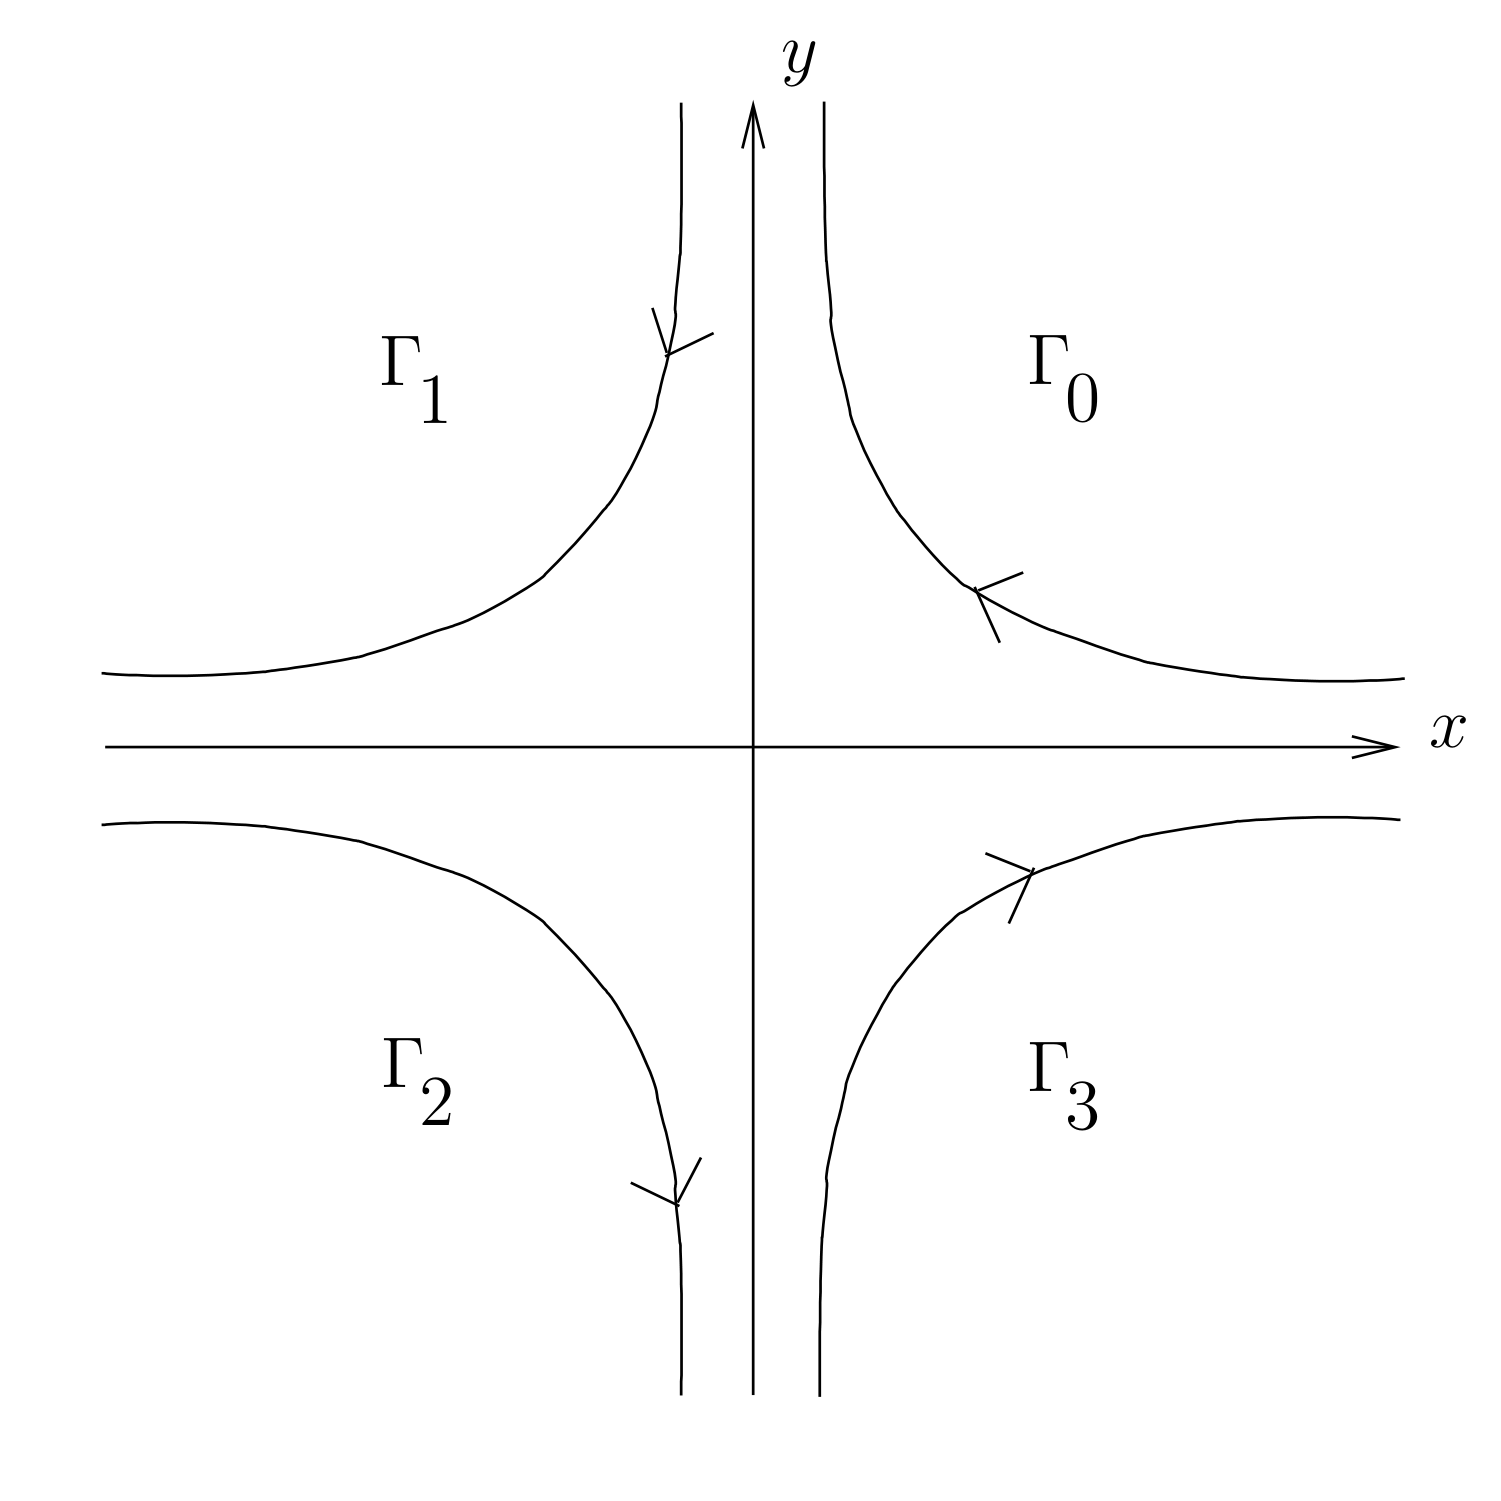
\includegraphics[width=0.46\textwidth]{figures/fig1_cycles.png}
  \caption{式 (1.5) 中积分 $I_{\Gamma}$ 的积分围道。四条围道满足一个关系
    $\Gamma_{0}+\Gamma_{1}+\Gamma_{2}+\Gamma_{3}=0$，其中任意三条都给出所有可能积分围道
    所成空间的一组基。（原文 Fig.~1，见英文版 p.~4；原图注印作
    “$\Gamma_{1}+\Gamma_{1}+\Gamma_{2}+\Gamma_{3}=0$”，其中第一个 $\Gamma_1$ 应为
    $\Gamma_{0}$，系笔误，详见批注。）}
  \label{fig:cycles}
\end{figure}

% [Tutor Note: 图注与正文在计数上有一个容易混淆之处，务必分清。复 $z$ 平面上共有四个
% 当 $|z|\to\infty$ 时 $\Re S\to-\infty$ 的"谷"，标为 $k=0,1,2,3$；相邻两谷之间的围道
% 记作 $\Gamma_k$（连接第 $k$ 谷与第 $k+1$ 谷），故有 $\Gamma_0,\Gamma_1,\Gamma_2,\Gamma_3$
% 四条，它们满足唯一关系 $\sum_{k=0}^{3}\Gamma_k=0$（因为四条围道首尾相接构成一条闭合
% 的大围道，而整函数沿闭围道积分为零）。原文图注误将 $\Gamma_0$ 印成 $\Gamma_1$，
% 若照抄会得到"$\Gamma_1$ 出现两次"的错误关系。正文说"本质上只有三条"，是指独立围道
% 数为 $4-1=3$，与相对同调的秩为三一致。另请注意：原文用 $I$ 同时表示作用量 (1.1)、
% 一维积分 (1.3) 与围道积分 $I_\Gamma$ (1.5)，阅读时须按上下文区分；本译文一律保留
% 原符号以免与公式编号混淆。]

给定 $n$ 维的类似积分
\begin{equation}
  \int_{\R^{n}} \dd x_{1}\dd x_{2}\cdots \dd x_{n}\; \exp\bigl(S(x_{1},\dots,x_{n})\bigr)\,,
  \tag{1.6}
\end{equation}
同样取适当的多项式 $S$，就可以把变量从实 $x_{i}$ 解析延拓到复 $z_{i}=x_{i}+\ii y_{i}$，
并把 (1.6) 换成沿某个适当积分围道 $\Gamma\subset\C^{n}$ 的积分：
\begin{equation}
  \int_{\Gamma} \dd z_{1}\dd z_{2}\cdots \dd z_{n}\; \exp\bigl(S(z_{1},\dots,z_{n})\bigr)\,.
  \tag{1.7}
\end{equation}
合适的积分围道是 $n$-维闭链，这仅仅是因为我们要积分的对象是 $n$-形式
$\dd z_{1}\dd z_{2}\cdots \dd z_{n}\,\exp(S(z_{1},\dots,z_{n}))$。当然，我们所要积分的
微分形式之所以是“中间维数”的，仅仅是因为在从 $\R^{n}$ 解析延拓到 $\C^{n}$ 时，我们把
积分所在空间的维数加倍了。于是，在实的情形中原本是最高维的微分形式，在解析延拓之后
就变成了中间维数的微分形式。

% [Tutor Note: "中间维数（middle-dimensional）"是理解全文的关键：$n$ 维复空间实维数为
% $2n$，$n$-形式恰是中间维数，只有中间维数的闭链才可能有自然的配对流（相交数）。
% 后文把这一套搬到环路空间：相空间 $M$（实 $2n$ 维）的环路空间复化后，伪全纯映射的
% 边界值给出其中间维数的闭链，这正是 Floer 同调的出发点（见 [10] 以及 [17] Gromov 的
% 伪全纯曲线理论）。]

在文献 [2] 中已经证明：至少在三维陈--西蒙斯规范理论的情形，这些概念可以有效地应用于
费曼积分这样的无穷维情形。但这样做我们能学到什么？当我们为同一个积分——或同一条路径
积分——构造出不同的积分围道时，所得的积分之间有何关系？一个答案可以回到最初的例子
$I_{\Gamma}$。无论 $\Gamma$ 如何选取（只用到它是无边的闭链、且其两端落在被积函数快速
衰减的区域，从而可以分部积分），$I_{\Gamma}$ 都满足微分方程
\begin{equation}
  \left(\frac{\dd^{3}}{\dd a^{3}} - a\right) I_{\Gamma} = 0\,.
  \tag{1.8}
\end{equation}
的确，当 $\Gamma$ 跑遍三个独立积分围道的选择时，$I_{\Gamma}$ 给出这个三阶微分方程解空间
（三维）的一组基。

% [Tutor Note: 式 (1.8) 的推导是 Picard--Lefschetz 理论的典型练习，也是全文"围道无关性"
% 的技术原型，极易出错，建议自行核对：(i) 对 $I_\Gamma(a)=\int_\Gamma \ee^{-z^4/4+az}\dd z$
% 求 $\dd/\dd a$ 会在被积函数中带下 $z$；(ii) 利用 $\frac{\dd}{\dd z}\ee^{S}=-\bigl(z^3-a\bigr)\ee^{S}$
% （注意 $S'=-z^3+a$）把 $z^3\ee^S$ 写成全导数加 $a\ee^S$；(iii) 沿 $\Gamma$ 的全导数项
% 因两端 $\Re S\to-\infty$ 而消失，于是得 $\bigl(\dd^3/\dd a^3-a\bigr)I_\Gamma=0$。
% 符号上最易错的是 $S'=-z^3+a$ 的负号：若误作 $S'=z^3-a$，会得到
% $(\dd^3/\dd a^3+a)I_\Gamma=0$，其特征值随之改变。另外"三个独立围道给出解空间的一组基"
% 用到相对同调与 de Rham 上同调的配对（周期映射），并非显然。]

对量子场论而言，(1.8) 的类比是关联函数所满足的 Ward 恒等式。与 (1.8) 一样，它们可由
函数空间中的分部积分证明，且不依赖于积分围道的选择。人们也许会认为，不同的积分围道
对应于同一量子理论中不同的真空态，但这并不总是对的。在某些情形（如我们将在 2.4 节用
一个显例说明的），不同的积分围道对应于具有相同可观测量代数的\textbf{不同量子系统}；
在另一些情形，其诠释则更为奇特。

% [Tutor Note: 这一段是全文的"哲学底线"，也是审稿人最容易被误导的地方：不要想当然地把
% "不同围道 = 不同真空"。Witten 明确指出反例（2.4 节的谐振子型例子），此时不同围道给出
% 的是同一代数但不同表示/不同谱的量子系统。读 2.4 节时请特别留意这一点。]

本文的第一个目标，是把这些想法应用于费曼路径积分中一个格外基本的情形，即非相对论量子
力学中坐标为 $q$、动量为 $p$ 的相空间路径积分：
\begin{equation}
  \int \mathcal{D}p(t)\,\mathcal{D}q(t)\;
  \exp\left(\ii \int \bigl(p\,\dd q - H(p,q)\,\dd t\bigr)\right).
  \tag{1.9}
\end{equation}
（$H(p,q)$ 是哈密顿量，在我们的视角下只起次要作用。）这一积分的积分围道将在第 2 节中
分析。有一些相当标准的积分围道，例如费曼最初假定的、$p(t)$ 与 $q(t)$ 均取实值的围道。
本文的主要新想法是：把积分限制在复值路径 $p(t),q(t)$ 上，而这些复值路径是伪全纯映射的
边界值——其确切含义并不显然——由此可以得到量子力学路径积分中一种新类型的积分围道。
此外，这条围道在二维量子场论中有自然的解释：那是一个以原经典相空间的复化为靶空间的
$\sigma$-模型。该 $\sigma$-模型实际上是一个拓扑扭曲的 A-模型，而这条积分围道可以用一种
奇特类型的 A-膜——所谓\textbf{余各向同性膜}（coisotropic brane）——来描述 [3]。

% [Tutor Note: 式 (1.9) 有两个经典陷阱，复化时尤其致命，务必留意：(1) 相空间路径积分的
% 测度 $\mathcal{D}p\,\mathcal{D}q$ 与 $p\,\dd q$ 这一项的配对，在 $(p,q)$ 复化后
% $p\,\dd q$ 不再自动是"实一次形式"，沿复围道积分时需要指定 $p$ 与 $q$ 的极化
% （polarization）选择；(2) $p\,\dd q$ 与 $-q\,\dd p$ 相差全微分 $\dd(pq)$，在开围道上
% 这一全微分项会给出非零边界项，因此"选哪条围道"与"作用量差一个全微分"这两件事必须
% 一起考虑——这正是后文 2.2、2.3 节要用 $u$、$v$ 等辅助变量仔细处理的地方。
% 另外，"伪全纯映射的边界值"一句作者自称"in a not obvious sense"，其确切含义是：
% 把时间方向视为二维曲面（如柱面 $\R\times I$ 或圆盘）的边界之一，映射到复化相空间，
% 并要求映射在内部的某组近复结构下伪全纯；其边界值即给出环路空间中的中间维闭链。
% 严格背景见 Floer [10] 与 Gromov [17]，场论视角见 [11–13]。]

从多种视角早已知道 [4--9]，A-模型与量子化之间存在联系。在本文中，我们对“关键联系究竟
是什么”提出了一个新的、格外直接的方案：最基本的余各向同性 A-膜给出了量子力学费曼积分
中的一条新积分围道。

伪全纯映射的边界值给出辛流形（或经典相空间）环路空间中的中间维闭链，这一事实是 Floer
上同调的主要思想之一 [10]。从场论角度的研究见 [11--13]。Floer 理论中的中间维闭链通常
并不被解释为积分围道，因为通常并不存在可以在这类闭链上积分的自然中间维形式。在本文中，
我们首先把维数加倍——把经典相空间复化——于是通常费曼积分的被积函数变成一个中间维形式，
从而可以在复化相空间的 Floer 理论所给出的闭链上积分。

% [Tutor Note: 这段是本文与既有文献 [10–13] 的分水岭，值得在此停顿：Floer 理论中
% 中间维闭链上没有自然形式可积，通常只用于定义相交数/Floer 同调；Witten 的做法是
% "把维数加倍"（复化相空间，实维数从 $2n$ 变 $4n$，中间维数从 $2n$ 变……注意这里
% 微妙：复化后复维数 $2n$，实维数 $4n$，欲积分的 $2n$-形式恰为复中间维），从而
% 让 $\dd p\,\dd q\,\ee^{\ii\oint p\dd q}$ 成为可积的中间维形式。若把"加倍"理解成
% 实维数加倍而忘记复结构，会算错维数配对，这是阅读第 2.6–2.7 节时最常见的错误。]

我们所描述的一维与二维理论之间的关系，在三维与四维之间有类比。这里三维理论是规范群
$G$ 紧致的陈--西蒙斯规范理论，四维理论则是具有同一规范群的 $\mathcal{N}=4$ 超杨--米尔斯
理论。两种理论之间的联系在某种程度上已由 [2] 建立：那里证明了，为了在三维陈--西蒙斯
理论中定义一条积分围道，有用的做法是添加第四个变量，并求解某些与四维 $\mathcal{N}=4$
超杨--米尔斯理论相关的偏微分方程。本文则更进一步，确切地证明：带边界的四维流形上
$\mathcal{N}=4$ 超杨--米尔斯理论的量子路径积分，如何能在边界上重现具有某条特定积分
围道的陈--西蒙斯路径积分。

这一结果有一个应用，将在别处 [14] 描述。该应用涉及一种新的方式来理解膜的 BPS 态 [15]
与纽结的 Khovanov 同调 [16] 之间的联系。

本文第 2、3 节从量子力学的标准费曼积分出发，进一步阐明它与一维扭曲超对称理论的关系。
在第 4 节中，我们把同一个故事反过来讲：从较高维出发，推导出它与低一维的标准费曼积分
之间的关系。有些读者可能更喜欢这第二种解释。第 5 节把这一方法推广到规范场，并包含
对陈--西蒙斯理论的应用。

带有奇特积分围道的费曼积分，其物理诠释是什么？在本文中我们对此不作任何断言，只指出
它以某种有趣的方式把一维与二维（或三维与四维）的信息联系了起来。

% [Tutor Note: 结尾这句"不作任何断言"是 Witten 一贯的谨慎措辞，读者不应据此认为该构造
% 缺乏物理意义——恰恰相反，这正是 [14]（Fivebranes and Knots）中 BPS 态/Khovanov 同调
% 应用的伏笔。另请注意本节的文献编号 [4–9] 对应正文中的 "coisotropic brane" 与
% "A-model 与量子化"两条线索，[10] 是 Floer 的原始文章，[17] 是 Gromov 的伪全纯曲线
% 奠基工作；这些是读懂第 2 节的最低文献配置。]


% ===== 片段：sections/s02a.tex =====

% 本片段覆盖 PDF p.7（§2 标题起）至 p.12 顶部（2.4 节标题之前），即印刷页 6–11。
% 原文：E. Witten, arXiv:1009.6032v1, §2.1–2.3。公式 (2.1)–(2.20) 逐一对应原文。

\section{量子力学的积分围道}

\begin{keypoints}
    \item \textbf{物理图像：}把通常的费曼路径积分解析延拓到经典相空间的复化；被积函数于是成为复化环路空间上的一个中维数形式，可以沿远比原来更一般的积分围道来积分。
    \item \textbf{数学工具：}带反全纯对合 $\tau$ 的复化辛流形 $(\widehat{\mathcal{M}},\Omega)$、分解 $\Omega=\omega+\mathrm{i}f$、预量子化线丛与狄拉克条件，以及作为完备性判据的 A-模型。
    \item \textbf{关键结论：}费曼积分的被积函数可以内蕴地写成 $\exp(\mathrm{i}\oint b_a\,\mathrm{d}x^a)$ 的形式；解析延拓后沿任意中维数闭链 $\Gamma$ 的积分 (2.20) 是本文的研究对象，而取 $\Gamma=\mathcal{U}$ 时它回到原来的费曼积分（式 (2.17)）。
    \item \textbf{记号提醒：}本节用 $f$ 而非通行的 $\omega$ 表示实相空间上的辛形式；$\omega$ 直到式 (2.11) 才作为复化辛形式 $\Omega$ 的实部出现。
\end{keypoints}

\subsection{预备知识}

一个经典力学系统由一个 $2n$ 维相空间 $\mathcal{M}$ 描述，$\mathcal{M}$ 上赋有辛结构。辛结构由一个闭的二维形式 $f$ 描述：
\begin{equation}
    \mathrm{d}f = 0,
    \tag{2.1}
\end{equation}
并且 $f$ 还是非退化的。所谓非退化，是指在局部坐标 $x^a$（$a=1,\dots,2n$）中由
$f=\sum_{a<b}f_{ab}\,\mathrm{d}x^a\wedge\mathrm{d}x^b$ 所定义的矩阵 $f_{ab}$ 可逆；我们把它的逆矩阵记为 $f^{ab}$。局部地，若 $f$ 是闭的非退化二维形式，则可以选取正则坐标 $p_r$、$q^s$（$r,s=1,\dots,n$），使得
\begin{equation}
    f = \sum_{s=1}^{n}\mathrm{d}p_s\wedge\mathrm{d}q^s .
    \tag{2.2}
\end{equation}

% [Tutor Note: 符号约定（印刷页 6–9）：Witten 用 $f$ 而不是通行的 $\omega$ 表示实相空间上的辛形式；到 §2.3 引入复化辛形式后写 $\Omega=\omega+\mathrm{i}f$，此时 $\omega$ 是 $\Omega$ 的实部。同一个字母 $\omega$ 在其它文献中常被用作辛形式，阅读时必须按本文约定，否则 (2.11)–(2.13) 会全部理解错。另：式 (2.2) 的局部存在性是达布（Darboux）定理，原文只写 "one can pick"，未给证明，可查任一辛几何标准教材。]

$\mathcal{M}$ 上两个函数 $u$、$v$ 的泊松括号定义为
\begin{equation}
    \{u,v\}
    = f^{ab}\frac{\partial u}{\partial x^a}\frac{\partial v}{\partial x^b}
    = \sum_{s}\left(\frac{\partial u}{\partial q^s}\frac{\partial v}{\partial p_s}
    -\frac{\partial u}{\partial p_s}\frac{\partial v}{\partial q^s}\right).
    \tag{2.3}
\end{equation}

% [Tutor Note: 式 (2.3) 的指标位置极易写错：$f^{ab}$ 是 $f_{ab}$ 之逆矩阵，$q^s$ 与 $p_s$ 的上下标必须互补；第二式的两项次序为 $(\partial_{q^s}u)(\partial_{p_s}v)-(\partial_{p_s}u)(\partial_{q^s}v)$，与 $\{q^s,p_s\}=1$ 的约定一致。若把 $p_s$ 误写成 $p^s$，或把两项次序颠倒，会整体差一个符号。]

在量子化中，人们希望为这些数据指派一个希尔伯特空间 $\mathcal{H}$ 和一个可观测量代数 $\mathcal{R}$。$\mathcal{H}$ 是有限维的，当且仅当 $\mathcal{M}$ 具有有限体积。在这种情形下，对 $\mathcal{R}$ 的元素 $U_1,\dots,U_n$，可以联系一个迹
\begin{equation}
    \operatorname{Tr}_{\mathcal{H}}U_1U_2\cdots U_n,
    \tag{2.4}
\end{equation}
它在酉等价的意义下刻画了 $\mathcal{R}$ 及其在 $\mathcal{H}$ 上的作用。在大多数物理应用中，$\mathcal{R}$ 中有一个称为哈密顿量的元素 $H$，而人们尤其关心形如
\begin{equation}
    \operatorname{Tr}_{\mathcal{H}}U_1(t_1)U_2(t_2)\cdots U_n(t_n)\exp(-\mathrm{i}Ht),
    \tag{2.5}
\end{equation}
的迹，其中对 $U\in\mathcal{R}$，$U(t)$ 定义为 $\exp(-\mathrm{i}Ht)U\exp(\mathrm{i}Ht)$。然而，量子化的基本问题\footnote{这一问题的许多初等面向并不像它们本可以的那样为人熟知。例如，从经典力学到量子力学的过渡并不把泊松括号映为对易子，除非在 $\hbar$ 的领头阶（本文取 $\hbar=1$）以及某些特殊情形，例如 $\mathcal{M}$ 上的二次函数。可参看 [9] 的评述。}在于为 $\mathcal{M}$ 指派希尔伯特空间 $\mathcal{H}$ 与代数 $\mathcal{R}$；本文关于这个问题的讨论，大多与 $H$ 的选取无关。我们将略去 $H$（即令 $H=0$），第 3 节除外。

% [Tutor Note: 原文用 $\mathcal{H}$（希尔伯特空间）与 $H$（哈密顿量）两个仅靠字体区分的符号，印刷页 7 甚至有 "if $\mathcal{M}$ has infinite volume, $\mathcal{H}$ is infinite-dimensional" 一句——若把其中的 $\mathcal{H}$ 误读成 $H$ 就完全说不通（已核对 PDF p.8 图像，确为花体 $\mathcal{H}$，不是笔误）。另注意 (2.5) 的时间演化约定 $U(t)=e^{-\mathrm{i}Ht}Ue^{\mathrm{i}Ht}$：指数上 $-\mathrm{i}Ht$ 在左、$+\mathrm{i}Ht$ 在右，与 $\operatorname{Tr}_{\mathcal{H}}(U_1\cdots U_n\,e^{-\mathrm{i}Ht})$ 中整体因子 $e^{-\mathrm{i}Ht}$ 的顺序一致。]

% [Tutor Note: 原文 "$\mathcal{H}$ 是有限维的当且仅当 $\mathcal{M}$ 具有有限体积"（印刷页 7）未加证明，是半经典态计数：每个量子态在相空间中占据体积 $(2\pi\hbar)^n$，故 $\dim\mathcal{H}\sim\operatorname{Vol}(\mathcal{M})/(2\pi\hbar)^n$。严格的陈述依赖量子化方案（几何量子化中紧致辛流形给出有限维表示），无限体积流形一般给出无限维表示；原文此处只需这一直观。]

对量子力学而言，一个更深刻的进路是：不仅考虑如 (2.5) 那样的迹，还考虑初、末量子态 $|\psi_i\rangle$、$|\psi_f\rangle$ 之间的矩阵元 $\langle\psi_f|U_1U_2\cdots U_n|\psi_i\rangle$。（这也避开了如下技术困难：若 $\mathcal{M}$ 具有无限体积，则 $\mathcal{H}$ 是无限维的，而 (2.4)、(2.5) 中的迹可能发散，视 $U_i$ 与 $H$ 而定。）然而，本文处理费曼积分的方法，若从迹而不是从矩阵元出发，解释起来最为方便。描述初、末态之间矩阵元所需的额外步骤，在第 2.10 节中概述。

\subsection{基本的费曼积分}

基本的费曼积分把迹 (2.4) 表示成从 $S^1$ 到 $\mathcal{M}$ 的映射的积分：
\begin{equation}
    \operatorname{Tr}_{\mathcal{H}}U_1U_2\cdots U_n
    = \int_{\mathcal{U}}Dp_r(t)\,Dq^r(t)\,
    \exp\left(\mathrm{i}\oint p_s\,\mathrm{d}q^s\right)
    u_1(t_1)u_2(t_2)\cdots u_n(t_n).
    \tag{2.6}
\end{equation}
这里 $p_r(t)$ 与 $q^r(t)$ 是周期的，周期可取为（例如）$2\pi$，因此它们定义一个映射 $\mathcal{T}:S^1\to\mathcal{M}$，换言之，即 $\mathcal{M}$ 的自由环路空间（free loop space）$\mathcal{U}$ 中的一个点。$u_\alpha$ 是 $\mathcal{M}$ 上的函数，量子化后对应于算子 $U_\alpha$。我们为每个函数 $u_\alpha$ 指定了一个时间 $t_\alpha$；但由于已经取哈密顿量为零，关于 $t_\alpha$ 唯一有意义的信息只是它们在 $S^1$ 上的循环次序。按惯例，$u(t)$ 是 $u(\mathcal{T}(t))$ 的简写。

% [Tutor Note: (2.6) 中的 $\oint$ 指沿参数圆 $S^1$ 的回路积分（时间方向），不是复平面上的围道积分；$p_s\,\mathrm{d}q^s$ 中重复指标 $s$ 求和。注意测度是 $Dp_r(t)Dq^r(t)$，其中 $r$ 也是重复指标。$u_\alpha$ 只是乘在指数因子之后的普通函数，不含时间演化算子——这正是"已取 $H=0$"的含义。]

如上所写，费曼积分依赖于正则坐标 $q^r$ 与动量 $p_r$ 的选取。例如，我们可以作从 $p,q$ 到 $-q,p$ 的正则变换，把 $\oint p_s\,\mathrm{d}q^s$ 换成 $-\oint q^s\,\mathrm{d}p_s$。这相当于在路径积分的指数上添加一项 $\oint\mathrm{d}(-p_sq^s)=0$；它为零是因为这些函数在时间上是周期的。

% [Tutor Note: "$\oint\mathrm{d}(-p_sq^s)=0$" 的依据是：恰当形式沿闭路的积分只依赖端点，而 $p$、$q$ 以 $2\pi$ 为周期，端点重合，故积分为零。这正是"换一组正则坐标不改变路径积分"的机制；原文 "the vanishing holds because the functions are periodic in time" 略去的正是这一步。]

与其选取某一组特定的正则坐标，一个更内蕴的做法是注意到：由于二维形式 $f$ 是闭的，它可以被看作一个阿贝尔规范场 $b$ 的曲率：
\begin{equation}
    f = \mathrm{d}b,\qquad b=\sum_{a=1}^{2n}b_a\,\mathrm{d}x^a .
    \tag{2.7}
\end{equation}
于是我们可以把 (2.6) 更内蕴地写成
\begin{equation}
    \operatorname{Tr}_{\mathcal{H}}U_1U_2\cdots U_n
    = \int_{\mathcal{U}}Dx^a(t)\,
    \exp\left(\mathrm{i}\oint b_a\,\mathrm{d}x^a\right)
    u_1(t_1)u_2(t_2)\cdots u_n(t_n).
    \tag{2.8}
\end{equation}

若 $f$ 的周期都是 $2\pi$ 的整数倍，我们就说狄拉克条件成立。在这种情形下，存在一个酉线丛 $\mathfrak{L}\to\mathcal{M}$，其上有一个曲率为 $f$ 的联络；我们取 $b$ 为该联络，其结构群为 $U(1)$。$\mathfrak{L}$ 称为预量子线丛（prequantum line bundle）。若 $H_1(M,\mathbb{Z})\neq0$，则 $\mathfrak{L}$ 有不等价的选择，而量子化依赖于这种选择。当 $\mathfrak{L}$ 存在时，因子 $\exp(\mathrm{i}\oint b_a\,\mathrm{d}x^a)$ 就是 $\mathfrak{L}$ 上联络 $b$ 的和乐（经由映射 $\mathcal{T}:S^1\to\mathcal{M}$ 拉回到 $S^1$）。

% [Tutor Note: "periods of $f$"（$f$ 的周期）指 $f$ 沿所有闭 2-链的积分；Dirac 条件即 $\int_{Z}f\in2\pi\mathbb{Z}$ 对一切闭 2-链 $Z$ 成立。原文写 $H_1(M,\mathbb{Z})\neq0$（注意这里的 $M$ 用的是斜体 $M$，而非前文的 $\mathcal{M}$，属原文记号不一致，照录）。曲率 $f$ 固定后，预量子线丛的不等价选择由平坦 $U(1)$ 线丛分类，即由 $\operatorname{Hom}(H_1(M,\mathbb{Z}),U(1))$ 分类，所以判据确实是 $H_1$；若按"线丛由第一陈类 $H^2(M,\mathbb{Z})$ 分类"去想，会误以为原文写错了。另：$\mathfrak{L}$ 是原文的花体 L（\verb|\mathfrak{L}|），不是 $\mathcal{L}$。]

若狄拉克条件不成立，则带有通常积分围道（integration cycle；此处为实相空间坐标 $x^a$）的费曼积分没有意义，因为路径积分中的因子 $\exp(\mathrm{i}\oint b_a\,\mathrm{d}x^a)$ 定义不良。把 $\mathcal{U}$ 换为它的万有覆盖——或换为任一使路径积分被积函数单值的覆盖 $\mathcal{U}^*$——可以使这个因子定义良好。一旦如此，费曼积分沿通常积分围道的积分便没有意义，因为所有积分 (2.6) 都为零。（在覆盖 $\mathcal{U}^*\to\mathcal{U}$ 的覆叠变换（deck transformation）下，它们相差一个非平凡相位变换。）然而，正如 [2] 中所分析、也如下文将要看到的，在解析延拓之后，可能存在有意义的积分围道（它们与形变量子化（deformation quantization）有关：形变量子化不要求狄拉克条件，而量子化要求）。因此我们并不想假设狄拉克条件成立。

% [Tutor Note: 上一段的"所有积分 (2.6) 都为零"是原文的断言，理由如下（原文未展开）：Dirac 条件不成立时，被积函数在覆盖 $\mathcal{U}^*\to\mathcal{U}$ 的覆叠变换下相差一个非平凡相位，故不同提升给出的积分没有覆叠变换不变的、自洽的数值；这一自由度正是 [2] 中"形变量子化不需要 Dirac 条件"的技术背景。]

在下文中，先在心里备一个例子或许会有帮助。一个简单的例子是 $\mathcal{M}=S^2$ 的情形，它由方程
\begin{equation}
    x_1^2+x_2^2+x_3^2 = j^2
    \tag{2.9}
\end{equation}
定义，其中 $j$ 为某个常数。我们取
\begin{equation}
    f = \frac{\epsilon_{ijk}x_i\,\mathrm{d}x_j\wedge\mathrm{d}x_k}{3!R^2}
    = \frac{\mathrm{d}x_1\wedge\mathrm{d}x_2}{x_3}.
    \tag{2.10}
\end{equation}
$f$ 的第一个表达式使 $SO(3)$ 不变性一目了然，第二个则便于计算。可以验证 $\int_{S^2}f=4\pi j$，于是狄拉克条件变为 $j\in\mathbb{Z}/2$。然而，如上文已经解释的，我们并不一定想假设这一条件。我们可以把 $f$ 看作由位于球心的磁单极子（磁荷为 $2j$）所产生的磁场；$b$ 就是这个单极子场的规范联络。

% [Tutor Note: 原文可疑/疑为笔误（印刷页 9，PDF p.10，式 (2.10)）：(2.9) 定义的是半径为 $j$ 的球面，而 (2.10) 第一式的分母印作 $3!R^2$，$R$ 在此前从未定义。用球面上的恒等式 $\epsilon_{ijk}x_i\mathrm{d}x_j\wedge\mathrm{d}x_k=2j^2\,\mathrm{d}x_1\wedge\mathrm{d}x_2/x_3$，第一式等于 $\frac{j^2}{3R^2}\frac{\mathrm{d}x_1\wedge\mathrm{d}x_2}{x_3}$；要它与第二式严格相等，必须 $3R^2=j^2$。而下一句的 $\int_{S^2}f=4\pi j$ 是由第二式（等价地取 $R=j/\sqrt3$）算出的；若取 $R=j$，会差因子 $1/3$。判断：$R$ 很可能是旧稿遗留的记号，本应换成 $j$（分母应为 $2R^2$ 且 $R=j$，或球面方程本应含 $3R^2$）。此处照原文抄录，请对照正式发表版核对；(2.19) 同一分母，问题相同。]

\subsection{解析延拓}

迄今为止我们所表述的费曼积分，是 $\mathcal{M}$ 的自由环路空间 $\mathcal{U}$ 上的积分，或者可能是它的某个使费曼积分的被积函数定义良好的覆盖上的积分。如引言所提示，我们的第一步是把 $\mathcal{U}$ 解析延拓到一个适当的复化 $\widehat{\mathcal{U}}$。我们只需选取 $\mathcal{M}$ 的一个复化 $\widehat{\mathcal{M}}$，并令 $\widehat{\mathcal{U}}$ 为 $\widehat{\mathcal{M}}$ 的自由环路空间（若有必要，则取其适当的覆盖）。

所谓 $\mathcal{M}$ 的复化，是什么意思？至少，$\widehat{\mathcal{M}}$ 应当是一个复流形，带有一个反全纯对合\footnote{对合（involution）就是平方等于恒等变换的对称性。} $\tau$，使得 $\mathcal{M}$ 是 $\tau$ 的不动点集的一个连通分支。此外，我们还希望 $\widehat{\mathcal{M}}$ 是一个复辛流形，赋有一个闭的非退化全纯二维形式 $\Omega$，并且具有如下性质：它的虚部限制到 $\mathcal{M}$ 上时与 $f$ 一致。我们通过
\begin{equation}
    \Omega = \omega+\mathrm{i}f
    \tag{2.11}
\end{equation}
引入 $\Omega$ 的实部与虚部。$\Omega$ 闭且非退化这一事实蕴含 $\omega$ 与 $f$ 各自闭且非退化。并且我们假设在 $\tau$ 作用下 $\Omega$ 被映为 $-\Omega$，换言之
\begin{equation}
    \tau^*(\omega) = -\omega,\qquad \tau^*(f) = f .
    \tag{2.12}
\end{equation}
% [Tutor Note: 正文 "$\Omega$ 闭且非退化蕴含 $\omega$ 与 $f$ 各自闭且非退化" 的前半显然（取实部、虚部），后半是原文的断言，值得补出证明：$\Omega$ 是 $(2,0)$ 形式，故对实向量 $u,v$ 有 $\Omega(u,Jv)=\mathrm{i}\,\Omega(u,v)$，从而 $\omega(u,Jv)=-f(u,v)$、$f(u,Jv)=\omega(u,v)$。若 $\omega$ 退化，取非零实向量 $u$ 使 $\omega(u,\cdot)=0$，则由前一式得 $f(u,\cdot)=0$，于是 $\Omega(u,\cdot)=0$，与 $\Omega$ 非退化矛盾；$f$ 同理。此论证同时说明为何可以放心地把 $\widehat{\mathcal{M}}$ 当作以 $\omega$ 为辛结构的实辛流形。]
由此可知，在不动点集 $\mathcal{M}$ 上 $\omega$ 必须为零：
\begin{equation}
    \omega|_{\mathcal{M}} = 0 .
    \tag{2.13}
\end{equation}

% [Tutor Note: 术语（印刷页 9）：反全纯对合 = antiholomorphic involution；不动点集 = fixed point set；复化 = complexification。注意 $\tau$ 是 $\widehat{\mathcal{M}}$ 上的实结构（real structure），其不动点集是实流形；"$\mathcal{M}$ 是固定点集的一个连通分支"这一措辞意味着允许 $\tau$ 还有别的分支（例如复化可能含多个实形式）。]
% [Tutor Note: 由 (2.12) 推出 (2.13) 只用了一个事实：$\tau$ 在不动点集 $\mathcal{M}$ 上诱导恒等映射，故对 $x\in\mathcal{M}$ 有 $(\tau^*\omega)_x=\omega_x$；与 $\tau^*\omega=-\omega$ 比较即得 $\omega|_{\mathcal{M}}=0$。这不是任何复化都自动满足的，而是对复化方式的实质限制：$\mathcal{M}$ 是 $(\widehat{\mathcal{M}},\omega)$ 的拉格朗日子流形，$\dim_{\mathbb{R}}\mathcal{M}=\tfrac12\dim_{\mathbb{R}}\widehat{\mathcal{M}}$。]

我们把 $\widehat{\mathcal{M}}$ 上的局部复坐标记为 $X^a$，其复共轭记为 $\overline{X}^a$；并把一组完备的局部实坐标（例如 $X^a$ 的实部与虚部）记为 $Y^A$。由于 $\Omega$ 是闭形式，我们可以把它写成一个复值阿贝尔规范场的曲率：
\begin{equation}
    \Omega = \mathrm{d}\Lambda,\qquad \Lambda=\sum_{A}\Lambda_A\,\mathrm{d}Y^A .
    \tag{2.14}
\end{equation}

% [Tutor Note: (2.14) 用的是 Poincaré 引理：闭形式局部恰当。$\Lambda$ 是复值 1-形式，各 $\Lambda_A$ 为复值分量，$A$ 取遍 $2\dim_{\mathbb{C}}\widehat{\mathcal{M}}$ 个实坐标（故与 $a$ 的个数不同，注意区分 $X^a$ 与 $Y^A$ 两套指标）。这里只是局部的陈述，并不声称 $\Lambda$ 整体存在。]

若原来的模型满足狄拉克条件，且复化不引入新的拓扑，则我们可以把 $\Lambda$ 视为结构群为 $\mathbb{C}^*$（$U(1)$ 的复化）的规范场。然而一般而言，如第 2.2 节所述，我们并不假设情况如此；我们改为把 $\widehat{\mathcal{U}}$ 换成一个适当的覆盖，使得下文引入的积分 (2.20) 的被积函数在这个覆盖上定义良好。方便起见，我们像对 $\Omega$ 所做的那样引入 $\Lambda$ 的实部与虚部，于是写成
\begin{equation}
    \Lambda = c+\mathrm{i}b,
    \tag{2.15}
\end{equation}
其中 $b$ 与 $c$ 是实值联络。因此
\begin{equation}
    \mathrm{d}c = \omega,\qquad \mathrm{d}b = f .
    \tag{2.16}
\end{equation}
我们将把 (2.13) 稍稍加强，假设存在一个规范使得
\begin{equation}
    c|_{\mathcal{M}} = 0 .
    \tag{2.17}
\end{equation}

% [Tutor Note: (2.17) 是对 (2.13) 的"加强"：由 $\mathrm{d}c=\omega$ 与 $\omega|_{\mathcal{M}}=0$，只知 $c|_{\mathcal{M}}$ 是闭 1-形式，一般未必为零；借规范变换 $\Lambda\to\Lambda+\mathrm{d}\chi$（$\chi$ 复值）可以局部地把 $c|_{\mathcal{M}}$ 消去，能否整体做到则取决于拓扑。引入 (2.17) 的用处见 (2.20) 之后：由 $\Lambda|_{\mathcal{M}}=\mathrm{i}b$，当 $\Gamma=\mathcal{U}$ 时 (2.20) 精确回到 (2.8)。]

下面针对 $\mathcal{M}=S^2$ 的例子说明这些定义的含义。我们用定义 $\mathcal{M}$ 时用过的同一方程 (2.9) 来定义 $\widehat{\mathcal{M}}$，只是\footnote{关于这种解析延拓在何种意义上自然或不自然、以及关于下文所考虑的可观测量类的批判性讨论，见 [9]。}现在把它看成关于复变量 $X_i$ 而不是实变量 $x_i$ 的方程：
\begin{equation}
    X_1^2+X_2^2+X_3^2 = j^2 .
    \tag{2.18}
\end{equation}
并且我们用与前面相同的公式定义 $\Omega$，只差一个因子 $\mathrm{i}$：
\begin{equation}
    \Omega = \mathrm{i}\,\frac{\epsilon_{ijk}X_i\,\mathrm{d}X_j\wedge\mathrm{d}X_k}{3!R^2}
    = \mathrm{i}\,\frac{\mathrm{d}X_1\wedge\mathrm{d}X_2}{X_3}.
    \tag{2.19}
\end{equation}
（在 $\Omega$ 的定义中出现因子 $\mathrm{i}$ 只是为了方便；若我们把 $f$ 取作 $\Omega$（限制到 $\mathcal{M}$ 上）的虚部而非实部，则随后的公式会略微优雅一些。）

% [Tutor Note: 注意 $\Omega$ 是复辛形式，而 (2.19) 里因子 $\mathrm{i}$ 的位置在分式之前（$\mathrm{i}\cdot\epsilon_{ijk}X_i\mathrm{d}X_j\wedge\mathrm{d}X_k/(3!R^2)$），不是分母中的 $\mathrm{i}$。由 (2.13) 得 $\Omega|_{\mathcal{M}}=\mathrm{i}f$，即 $f$ 是 $\Omega$ 在实切片上的虚部——这正是原文括号中那句话的意思。若把 (2.11) 写成 $\Omega=\omega-\mathrm{i}f$，或漏掉 (2.19) 的 $\mathrm{i}$，则 (2.16) 的 $\mathrm{d}b=f$ 与 $c|_{\mathcal{M}}=0$ 将不再自洽。]

除了我们已经陈述的条件之外，$\widehat{\mathcal{M}}$ 还必须具有一个额外的性质。关于 $\widehat{\mathcal{M}}$ 的某种完备性条件必定是需要的，因为若我们从 $\widehat{\mathcal{M}}$ 中挖去一个随意选取的、与 $\mathcal{M}$ 不相交的 $\tau$-不变闭集，显然不能指望得到好的理论。先验地看，正确的条件是什么并不显然；但我们将发现（[9] 中以另一种方式也已发现），适当的条件是：把 $\widehat{\mathcal{M}}$ 看作具有辛结构 $\omega$ 的实辛流形时，它必须有一个定义良好的 A-模型。对于非紧辛流形，这是一个非平凡、且一般而言尚未被很好理解的条件。我们关于 $S^2$ 复化的例子当然有一个好的 A-模型，因为这个流形事实上容许一个完备的超凯勒度规——Eguchi–Hansen 度规。

% [Tutor Note: "以 $\omega$ 为辛结构须有定义良好的 A-模型"是本节最实质、也最不显然的附加条件：它排除在无穷远处随意去掉 $\tau$-不变闭集所造成的不完备性。对非紧辛流形，"A-模型是否有定义"一般没有已知的充要判据，原文只引 [9]；$S^2$ 的复化（Eguchi–Hanson 空间）因容许可完全超凯勒度规而满足该条件。另：原文印刷页 11（PDF p.12）印作 "Eguchi-Hansen"，标准拼写为 Eguchi–Hanson，疑为原文笔误，此处译文保留原拼写并在此说明。]

至于出现在路径积分 (2.6) 中的那些函数 $u_\alpha$：要使它们在费曼积分的解析延拓的语境中有意义，它们必须能够解析延拓为 $\widehat{\mathcal{M}}$ 上的全纯函数（我们仍记作 $u_\alpha$）。此外，为了不影响涉及路径积分收敛性的问题，解析延拓后的函数在无穷远处不应增长过快。例如在 $S^2$ 的情形，多项式函数 $u(x_1,x_2,x_3)$ 是一类好的函数；这种多项式的解析延拓就是相应的多项式 $u(X_1,X_2,X_3)$。这些是最好考虑的可观测量，因为它们是在无穷远处增长最慢的（非常数）全纯函数。

把 $\mathcal{M}$ 的自由环路空间 $\mathcal{U}$ 解析延拓为 $\widehat{\mathcal{M}}$ 的相应复化环路空间 $\widehat{\mathcal{U}}$，并类似地解析延拓辛结构与可观测量之后，我们就可以形式地写出沿任意积分围道 $\Gamma\subset\widehat{\mathcal{U}}$ 的费曼积分：
\begin{equation}
    \int_{\Gamma}DY^A(t)\,\exp\left(\oint\Lambda_A\,\mathrm{d}Y^A\right)
    u_1(t_1)\cdots u_n(t_n).
    \tag{2.20}
\end{equation}
$\Gamma$ 是 $\widehat{\mathcal{U}}$ 中任一使该积分收敛的中维数闭链（middle-dimensional cycle）。式 (2.17) 保证：若取 $\Gamma$ 为费曼积分原来的积分围道 $\mathcal{U}$，则 (2.20) 确实与原来的费曼积分一致。

% [Tutor Note: 式 (2.20) 有两个不同层次的积分，切勿混淆：指数内部的 $\oint\Lambda_A\mathrm{d}Y^A$ 仍是沿参数圆 $S^1$ 的回路积分；外层的 $\int_\Gamma$ 是复化环路空间 $\widehat{\mathcal{U}}$（无限维）上的积分。"中维数闭链"（middle-dimensional cycle）指实维数等于 $\widehat{\mathcal{U}}$ 实维数一半的闭链，只有这样维数的闭链才能与 $e^{\oint\Lambda}$ 所给出的中维数形式配对得到有限数。由 (2.17) 的 $c|_{\mathcal{M}}=0$，当 $\Gamma=\mathcal{U}$ 时 $\oint\Lambda_A\mathrm{d}Y^A$ 限制到 $\mathcal{M}$ 上等于 $\mathrm{i}\oint b_a\mathrm{d}x^a$，故 (2.20) 化回 (2.8)——这就是末句"确实与原来的费曼积分一致"的含义。]


% ===== 片段：sections/s02b.tex =====

\subsection{最简单的积分围道}

% （本节重点见 §2 开头片段；本片段含 §2.4--§2.6，对应 PDF p.12--p.19，公式 (2.21)--(2.42)）

选取积分围道 $\Gamma$ 之所以有微妙之处，是因为式 (2.20) 中指数的实部没有上界。

式 (2.20) 中带来麻烦的因子来自 $\Lambda$ 的实部。（我们假定可观测量 $u_\alpha$ 的增长不至于快到会影响下面的讨论。）积分围道 $\Gamma$ 必须这样选取，使得危险因子
\begin{equation}
    \exp\left(\oint c_A\,\mathrm{d}Y^A\right)
    = \exp\left(\operatorname{Re}\oint \Lambda_A\,\mathrm{d}Y^A\right)
    \tag{2.21}
\end{equation}
不会使积分发散。它之所以麻烦，是因为指数
\begin{equation}
    h=\oint c_A\,\mathrm{d}Y^A
    \tag{2.22}
\end{equation}
既无上界也无下界。例如，映射
\begin{equation}
    Y^A(t)\to\tilde{Y}^A(t)=Y^A(nt)
    \tag{2.23}
\end{equation}
就把 $h$ 乘以一个任意的整数 $n$，而 $n$ 可正可负。

% [Tutor Note: p.11（PDF p.12）式 (2.22)--(2.23)：h=\oint c_A\mathrm{d}Y^A 关于环路 Y(t) 是一次泛函；重参数化 t\mapsto nt（式 (2.23)）使 \mathrm{d}Y^A 整体乘以 n，故 h\mapsto nh；令 n\to\pm\infty 即知 h 在 \widehat{\mathcal U} 上既无上界也无下界。这正是“围道不能随意取”的根源。式 (2.24) 的条件 \omega|_{\mathcal M_0}=0 则是把 h 限制在 \mathcal M_0 的环空间上成为常数，从而消除这一无界性。]

撇开收敛性问题不论，我们怎样找出一个中间维闭链 $\Gamma\subset\widehat{\mathcal U}$ 呢？最朴素的办法是用一个“逐时刻”（local-in-time）条件来定义 $\Gamma$：取一个中间维子流形 $\mathcal M_0\subset\widehat{\mathcal M}$，并取 $\Gamma\subset\widehat{\mathcal U}$ 为 $\mathcal M_0$ 的自由环空间。换言之，$\Gamma$ 参数化那些像始终落在 $\mathcal M_0$ 中的映射 $\mathcal T:S^1\to\widehat{\mathcal M}$。

这类选法不会出错，因为若取 $\mathcal M_0=\mathcal M$，我们就回到原来的费曼积分。现在要问：对 $\mathcal M_0$ 的哪些其他选法，我们仍能得到合适的积分围道？

当限制在 $\mathcal M_0$ 的环空间上时，函数 $h$ 必须恒为零；否则围绕式 (2.23) 的论证会再次表明它既无上界也无下界。$h$ 在映射 $\mathcal T:S^1\to\widehat{\mathcal M}$ 的小改变下的变分为
\begin{equation}
    \delta h=\oint \omega_{AB}\,\delta Y^A\,\mathrm{d}Y^B .
    \tag{2.24}
\end{equation}
要使它在 $\mathcal M_0$ 中任何环路上求值都恒为零，我们要求 $\omega$ 限制在 $\mathcal M_0$ 上为零。\footnote[5]{这已足以保证 $h$ 在 $\mathcal M_0$ 自由环空间的每个连通分支上为常数。要让它恒为零，我们还需要求 $c$ 限制在 $\mathcal M_0$ 上时为纯规范。}

% [Tutor Note: p.12 式 (2.24) 的推导：\delta h=\oint(\delta c_A\,\mathrm{d}Y^A+c_A\,\mathrm{d}\delta Y^A)，对第二项分部积分（用 \oint \mathrm{d}(c_A\delta Y^A)=0）得 -\oint \partial_B c_A\,\delta Y^A\mathrm{d}Y^B，合并即得 \oint(\partial_A c_B-\partial_B c_A)\delta Y^A\mathrm{d}Y^B=\oint\omega_{AB}\delta Y^A\mathrm{d}Y^B。故式 (2.24) 隐含取 \omega_{AB}=\partial_A c_B-\partial_B c_A，即 \omega=\mathrm{d}c（式 (2.16)）；若改用 \omega=-\mathrm{d}c 的约定，式 (2.24) 整体变号。此处指标位置与反对称化最易出错，务必与式 (2.16) 对照。]

% [Tutor Note: p.12 脚注 5：\omega|_{\mathcal M_0}=0 只保证 h 在每个连通分支上为常数；要 h 恒为零，还须 c|_{\mathcal M_0} 为纯规范。注意 \omega=\mathrm{d}c（式 (2.16)），故 h 只依赖于 \omega 的积分，而 h 的具体数值还依赖于 c 的规范选取——“常数”与“零”的差别正来源于此。]

换言之，我们要求 $\mathcal M_0$ 必须是关于 $\omega$ 的拉格朗日子流形。这是二维 $A$-模型中的一个熟悉条件：它是 $\mathcal M_0$（配以平凡的 Chan--Paton 丛）成为某个 $A$-膜之支撑的条件的经典近似。这不是巧合，而是第一个迹象，表明路径积分的可能积分围道与 $A$-模型有关。

在把 $\mathcal M_0$ 选得使路径积分指数的实部有上界之后，我们仍不能高枕无忧：为了使无穷维路径积分有意义，来自指数虚部的相位因子必须非退化。为此，我们希望 $f$ 限制在 $\mathcal M_0$ 上时非退化。换句话说，$\mathcal M_0$ 应当具有 $\mathcal M$ 的某些基本性质：限制在 $\mathcal M_0$ 上时，$\omega$ 为零而 $f$ 非退化。\footnote[6]{我们对 $\mathcal M$ 还施加过一个条件：$\mathcal M$ 是某个反全纯对合 $\tau$ 的不动点集的一个连通分支。如 [9] 所解释，这一条件是为了使 $A$-模型意义下的 $\mathcal M$ 量子化容有厄米结构。因此，若 $\mathcal M_0$ 不满足这一条件，它经由 $A$-模型的“量子化”——这一操作在 2.10 节中综述——就不是酉的。} 在这些条件下，取 $\Gamma$ 为 $\mathcal M_0$ 的环空间时，费曼积分 (2.20) 就恰好是原来以 $\mathcal M_0$ 代替 $\mathcal M$ 的费曼积分 (2.8)；换句话说，它就是与 $\mathcal M_0$ 的量子化相联系的通常费曼积分。

在这种情形下，$\mathcal M_0$ 的不同选法所对应的不同量子力学问题，恰好是同一个复化费曼积分中的不同积分围道。为了看清这件事如何具体发生，让我们回到熟悉的例子，其中 $\widehat{\mathcal M}$ 由方程
\begin{equation}
    X_1^2+X_2^2+X_3^2=j^2
    \tag{2.25}
\end{equation}
定义。对 $\mathcal M_0$ 的条件是 $\operatorname{Re}\Omega|_{\mathcal M_0}=0$，换言之
\begin{equation}
    \operatorname{Im}\left(\frac{\mathrm{d}X_1\wedge\mathrm{d}X_2}{X_3}\right)\bigg|_{\mathcal M_0}=0 .
    \tag{2.26}
\end{equation}
一个充分条件是 $X_1,X_2,X_3$ 全为实，这把我们带回原来的相空间 $\mathcal M$。为得到另一个例子，我们这样定义 $\mathcal M'$：要求 $X_1$ 为实且为正，而 $X_2$ 与 $X_3$ 为纯虚。不难看出，$\mathcal M$ 是二维球面 $S^2$，而 $\mathcal M'$ 则是上半平面 $H^2$ 的一个拷贝。无论量子化的是 $\mathcal M$ 还是 $\mathcal M'$，可观测量都一样，即限制在 $\mathcal M$ 或 $\mathcal M'$ 上的多项式 $u(X_1,X_2,X_3)$（模掉关系 (2.25)）。此外，这些可观测量的关联函数之间的任何恒等式（(2.25) 除外）都作为路径积分中的 Ward 恒等式出现，并可通过对场空间作分部积分来证明。因此，正如微分方程 (1.8) 那样，无论选取哪一条积分围道，同样的恒等式都成立。于是我们就得到了一对量子力学系统——分别联系于 $\mathcal M$ 与 $\mathcal M'$ 的量子化——它们具有相同的量子可观测量代数，但表示互不等价。

% [Tutor Note: p.13 式 (2.25)--(2.26)：由式 (2.19) 有 \Omega=\mathrm{i}\,\mathrm{d}X_1\wedge\mathrm{d}X_2/X_3，因此 \operatorname{Re}\Omega=-\operatorname{Im}(\mathrm{d}X_1\wedge\mathrm{d}X_2/X_3)。所以“$\operatorname{Re}\Omega|_{\mathcal M_0}=0$”与式 (2.26) 之间只差这个由因子 i 带来的整体符号；这是本节最容易抄错符号的一处，请按式 (2.19) 核对。]

% [Tutor Note: p.13--14 关于 \mathcal M'：取 X_1 实且为正、X_2,X_3 纯虚，方程 (2.25) 化为 X_1^2-Y_2^2-Y_3^2=j^2（其中 X_1>0，Y_{2,3}=\operatorname{Im}X_{2,3}），这正是双曲平面 H^2 的双叶双曲面模型的上叶，故原文称 \mathcal M' 是 H^2 的拷贝。两套理论的可观测量代数同为 \mathrm{sl}(2) 的泛包络代数，但二者之间的等价不保持厄米性：限制在 \mathcal M 上为实的多项式与限制在 \mathcal M' 上为实的多项式不同，故两个 $*$-表示不等价。这正是原文“same algebra of quantum observables, though with inequivalent representations”的确切含义。]

最后，关于这个例子我们还要作几点说明；这些在 [9] 中有更充分的解释，对本文则并非真正必要。具体说来，在经典层面，除 (2.25) 之外 $X_i$ 所满足的唯一关系就是它们彼此交换；量子化后，$X_i$ 的交换性被形变为 $\mathrm{sl}(2)$ 关系 $[X_1,X_2]=X_3$ 及其循环置换。（(2.25) 中的常数 $j^2$ 在量子层面也会被修正。）这意味着可观测量代数是 $\mathrm{sl}(2)$ 的泛包络代数——无论我们量子化的是 $\mathcal M$ 还是 $\mathcal M'$。这就具体解释了为什么这两个系统具有相同的可观测量代数。一个重要细节是：把量子化 $\mathcal M$ 所得的可观测量代数等同于量子化 $\mathcal M'$ 所得的可观测量代数的那个同构，并不把厄米算子映为厄米算子。最简单的理由是：限制在 $\mathcal M$ 上为实的那些多项式 $u(X_1,X_2,X_3)$，与限制在 $\mathcal M'$ 上为实的那些多项式并不相同。

在脚注 6 中我们曾指出，一般而言 $\mathcal M_0$ 可能不满足我们对原来的 $\mathcal M$ 所施加的某一个条件：可能不存在以 $\mathcal M_0$ 为不动点集的某个连通分支的反全纯对合。然而在 $\mathcal M'$ 的情形，这样的对合 $\tau'$ 确实存在，它作用为
\[
    X_1,X_2,X_3\to\overline{X}_1,\,-\overline{X}_2,\,-\overline{X}_3 .
\]
因此 $\mathcal M'$ 实际上满足 $\mathcal M$ 所满足的一切条件。两者之间的关系是完全对称的：我们可以认为 $\widehat{\mathcal M}$ 是由 $\mathcal M$ 或由 $\mathcal M'$ 解析延拓而来的。

% [Tutor Note: p.14 反全纯对合 \tau'：作用为 (X_1,X_2,X_3)\mapsto(\overline{X}_1,-\overline{X}_2,-\overline{X}_3)。注意后两个分量带负号与复共轭的组合（而不是简单复共轭），这是使不动点集包含 \mathcal M'（X_2,X_3 纯虚、X_1 实）的关键；抄写时极易漏掉负号或丢掉共轭。]

\subsection{莫尔斯理论回顾}

为了构造更有趣的积分围道，我们将使用莫尔斯理论与最速下降法。有关想法的详细综述见 [2]；这里我们给出一个简短的梗概，以使本文自成体系。

设 $Z$ 是一个 $m$ 维流形，局部坐标为 $w^i$，$i=1,\dots,m$，并带有一个莫尔斯函数 $h$。所谓莫尔斯函数，不过是一个实值函数，其临界点都非退化。$h$ 的临界点是指其各阶导数全为零的点 $p$。若二阶导数矩阵 $\partial^2h/\partial w^i\partial w^j$ 在 $p$ 处可逆，则称 $p$ 为 $h$ 的非退化临界点。此时该矩阵负特征值的个数称为 $h$ 在 $p$ 处的莫尔斯指数，我们把它记作 $i_p$。

取 $Z$ 上的一个 Riemann 度规 $g_{ij}\mathrm{d}w^i\mathrm{d}w^j$。引入“时间”坐标 $s$（我们把 $t$ 这个名字留给原量子力学问题中的时间，后面还要回到它），定义莫尔斯理论的流方程：
\begin{equation}
    \frac{\mathrm{d}w^i}{\mathrm{d}s}=-g^{ij}\frac{\partial h}{\partial w^j}.
    \tag{2.27}
\end{equation}
流方程的第一个性质是：沿任何非常数流，莫尔斯函数总是递减的，因为
\begin{equation}
    \frac{\mathrm{d}h}{\mathrm{d}s}
    =-g^{ij}\frac{\partial h}{\partial w^i}\frac{\partial h}{\partial w^j}.
    \tag{2.28}
\end{equation}
只要 $\partial h/\partial w^i\neq0$，右端就是负的；而在 $\partial h/\partial w^i=0$ 时，流在所有 $s$ 上都停在临界点。当然，这个论断依赖于度规 $g_{ij}\mathrm{d}w^i\mathrm{d}w^j$ 的正定性。$h$ 沿流递减这一事实，正是流方程会有用的原因。

% [Tutor Note: p.14 式 (2.27)--(2.28)：$g^{ij}$ 是度规 $g_{ij}$ 的逆矩阵，流方程取 $-\operatorname{grad}h$；由链式法则 \mathrm{d}h/\mathrm{d}s=(\partial_i h)(\mathrm{d}w^i/\mathrm{d}s)=-g^{ij}\partial_i h\,\partial_j h\le0，式 (2.28) 的负号即由此而来，并用到了 $g$ 的正定性。若度规号差或流的方向约定取反，后面“$h$ 在 $\mathcal C_p$ 上的最大值在 $p$ 处”等结论会随之全部改变，务必核对。]

让我们考察临界点 $p$ 邻域内的流。把二阶导数矩阵对角化之后，可以找到以 $p$ 为中心的 Riemann 正规坐标系 $w^i$，在其中
\[
    h=h_0+\sum_{i=1}^{m}e_i w_i^2+\mathcal O(w^3),
    \qquad g_{ij}=\delta_{ij}+\mathcal O(w^2),
\]
其中 $h_0,e_i$ 为常数。流方程化为
\begin{equation}
    \frac{\mathrm{d}w^i}{\mathrm{d}s}=-e_i w^i,
    \tag{2.29}
\end{equation}
其解为
\begin{equation}
    w^i=r^i\exp(-e_i s),
    \tag{2.30}
\end{equation}
其中 $r^i$ 为常数。流方程的一个解，如果并非在所有 $s$ 上都恒停在 $p$ 处（即 $w^i=0$ 处），那就只能在 $s=\pm\infty$ 到达 $p$。我们着重考察在 $s=-\infty$ 处从临界点 $p$ 出发的解。由式 (2.30) 显然可见，为此所需的条件是：凡 $e_i>0$，$r^i$ 必须为零。这样剩下 $i_p$ 个未定参数，所以从 $p$ 在 $s=-\infty$ 出发的解构成一个 $i_p$ 维族。我们定义 $Z$ 的一个 $i_p$ 维子空间 $\mathcal C_p$，它由从 $p$ 在 $s=-\infty$ 出发的流方程的解在 $s=0$ 处的取值组成。点 $p$ 本身属于 $\mathcal C_p$，因为它是恒停在 $p$ 处的平凡流在 $s=0$ 处的取值。由于 $h$ 沿任何非常数流严格递减，$\mathcal C_p$ 中 $h$ 的最大值就是它在 $p$ 处的值。

% [Tutor Note: p.15：这里的 $\mathcal C_p$（从 $p$ 在 $s=-\infty$ 出发的流在 $s=0$ 处的取值集合）按标准莫尔斯理论就是 $p$ 的不稳定流形 $W^u(p)$，其维数等于莫尔斯指数 $i_p$；而稳定流形 $W^s(p)$ 对应 $s\to+\infty$ 时收敛到 $p$ 的轨道。若把两者搞反，“剩下 $i_p$ 个未定参数”这一步就无法理解：由式 (2.30)，$e_i>0$ 的方向必须令 $r^i=0$（这些是稳定方向），能够自由取值的是 $e_i<0$ 的 $i_p$ 个不稳定方向。]

在有利的情形下，$\mathcal C_p$ 的闭包是同调闭链，它们生成 $Z$ 的同调。如 [2] 所综述，一个非常有利的情形是：$Z$ 是一个复流形，其复维数为 $n$、实维数为 $m=2n$，属于容许许多全纯函数的那一类，而 $h$ 是某个一般位置的全纯函数 $S$ 的实部。此时 $h$ 在非退化临界点 $p$ 附近的局部形式为
\[
    h=h_0+\operatorname{Re}\left(\sum_{i=1}^{n}z_i^2\right),
\]
其中 $z_i$ 为局部复坐标。命 $z_i=x_i+\mathrm{i}y_i$，其中 $x_i,y_i$ 为实，并注意 $\operatorname{Re}z_i^2=x_i^2-y_i^2$，即可看出 $h$ 的稳定方向与不稳定方向是成对的。因此，任何这样的 $p$ 的莫尔斯指数 $i_p$ 总等于 $n=m/2$，相应的 $\mathcal C_p$ 是中间维的。在这种情形下，对一般位置\footnote[7]{如 [2] 所解释，一个充分判据是不同临界点之间不存在流。由于 $\operatorname{Im}S$ 沿流线守恒，只要不同临界点（若临界点非孤立，则指临界集的不同连通分支）具有不同的 $\operatorname{Im}S$ 值，这一点就成立。存在临界点之间的流的例外情形会导致 Stokes 现象；Stokes 现象在 [2] 中很重要，但在本文中并不重要。}的 $S$，$\mathcal C_p$ 是闭的（但不紧），并且构成适当的相对同调群的一组基；这个相对同调群分类了使 $h$ 有上界且在无穷远处趋于 $-\infty$ 的闭链。

% [Tutor Note: p.15：$h=\operatorname{Re}S$ 时，在每个复方向 $z_i=x_i+\mathrm{i}y_i$ 上 $\operatorname{Re}z_i^2=x_i^2-y_i^2$ 给出特征值 $+1$ 与 $-1$ 的一对，因此稳定方向与不稳定方向成对，$i_p\equiv n=m/2$，$\mathcal C_p$ 恒为中间维。“closed but not compact”指其在无穷远处未必紧；脚注 7 说明若不同临界点之间存在流（即 $\operatorname{Im}S$ 在这些点取值相同），则出现 Stokes 现象，这正是标准莫尔斯--Smale 理论中用相对同调/复形（Witten 复形，见 [2]）处理的情形。可另参 Milnor《Morse Theory》第 3--7 节。]

现在取 $Z=\mathbb C^n$，考虑引言中描述的那类指数积分：
\begin{equation}
    \int_\Gamma \mathrm{d}z_1\,\mathrm{d}z_2\cdots\mathrm{d}z_n\,
    \exp\left(S(z_1,\dots,z_n)\right).
    \tag{2.31}
\end{equation}
令 $h=\operatorname{Re}S$，积分收敛的主要问题来自被积函数的模是 $\exp(h)$。只要沿 $\Gamma$ 在无穷远处 $h\to-\infty$，收敛性就有保证，因此上面描述的闭链 $\mathcal C_p$ 给出了“合理”积分围道空间的一组基。例如，让我们考虑引言中讨论过的一维积分：
\begin{equation}
    \int_\Gamma \mathrm{d}z\,\exp(S(z)),
    \qquad S(z)=-z^4/4+az.
    \tag{2.32}
\end{equation}

% [Tutor Note: p.15 式 (2.31)--(2.32)：$\mathrm{d}z_1\cdots\mathrm{d}z_n$ 是 $(n,0)$ 型复体积形式，而围道 $\Gamma$ 必须是实 $n$ 维的中间维闭链，两者维数恰好匹配；被积函数的模为 $\exp(h)$，故“沿 $\Gamma$ 在无穷远 $h\to-\infty$”正是收敛判据。对 $S(z)=-z^4/4+az$，临界点方程为 $\mathrm{d}S/\mathrm{d}z=-z^3+a=0$，有三个单根（$a\neq0$），所以可能的围道空间的秩为 3，与引言的图 1 一致。]

$h=\operatorname{Re}S$ 的临界点所满足的方程是三次方程 $\mathrm{d}S/\mathrm{d}z=0$。这个方程在复 $z$ 平面中有三个根，这与可能的积分围道空间秩为三这一事实一致，从引言中的图 1 可以明显看出。

在我们的应用中，莫尔斯函数 $h$ 将是某个全纯函数 $S$ 的实部，但它的临界点不是孤立的。上面的讨论因此需要作一些小的修改。设 $\mathcal N$ 是临界点集的一个连通分支。$\mathcal N$ 将是 $Z$ 的一个复子流形，设其复维数为 $r$；我们仍取 $Z$ 的复维数为 $n$。这时，与 $\mathcal N$ 垂直的方向有 $n-r$ 个复维数，即 $2(n-r)$ 个实维数。我们假定 $h$ 在垂直于 $\mathcal N$ 的方向上非退化，意思是 $h$ 的二阶导数矩阵在 $\mathcal N$ 上任一点处有 $2n-2r$ 个非零特征值。在这种情形下，$h$ 的局部形式为
\[
    h=h_0+\operatorname{Re}\sum_{i=1}^{n-r}z_i^2,
\]
而 $h$ 的二阶导数矩阵恰有 $n-r$ 个负特征值。在 $s=-\infty$ 时从 $\mathcal N$ 上出发的流方程的解所构成的空间 $\mathcal C_N$，其实维数为 $2r+(n-r)=n+r$：其中 $2r$ 个参数确定流在 $\mathcal N$ 上的起点，$n-r$ 个参数则来自流有 $n-r$ 个不稳定方向。于是，$\mathcal C_N$ 是一个高于中间维数的闭链。要得到中间维闭链，我们必须施加 $r$ 个条件，即要求流起始于 $\mathcal N$ 中的一个中间维闭链 $V$ 上。半直线 $(-\infty,0]$ 上从 $V$ 出发的流方程的解在 $s=0$ 处的取值，构成 $\mathbb C^n$ 中一个中间维闭链 $\mathcal C_V$。

% [Tutor Note: p.16：维数计数 $\dim\mathcal C_N=2r+(n-r)=n+r$ 是本节最易算错之处：$2r$ 来自流在 $\mathcal N$ 上的起点自由度（$\mathcal N$ 实维 $2r$），$n-r$ 来自法向的 $n-r$ 个不稳定方向（法向实维 $2(n-r)$，而 $h=\operatorname{Re}\sum z_i^2$ 在每对法向方向恰贡献一个负特征值）。要得到中间维闭链，须把起点限制在 $\mathcal N$ 的中间维闭链 $V$ 上，从而削减 $r$ 维——这正是 §2.6 中 $V\subset\widehat{\mathcal M}_*$ 的来源。]

让我们看一个简单的例子。取 $Z=\mathbb C^3$，并令
\begin{equation}
    S=(z_1^2+z_2^2+z_3^2-j^2)^2.
    \tag{2.33}
\end{equation}
于是 $S$ 在原点有一个孤立的非退化临界点。此外它还有由 $z_1^2+z_2^2+z_3^2=j^2$ 给出的一个临界点族 $\mathcal N$。$\mathcal N$ 的复维数为二，而 $h=\operatorname{Re}(S)$ 在垂直于 $\mathcal N$ 的方向上非退化。$\mathcal N$ 恰好等价于式 (2.18) 中引入的复流形 $\widehat{\mathcal M}$，所以作为 $\mathcal N$ 中中间维闭链的例子，我们可以取我们的老朋友 $\mathcal M$ 与 $\mathcal M'$——它们分别由要求 $z_i$ 为实，或要求 $z_1$ 为实且为正而 $z_2,z_3$ 为纯虚来定义。

\subsection{费曼积分的一个新积分围道}

希望至此已经清楚：在试图描述费曼积分的积分围道时，我们所处的正是刚刚描述的情形。费曼积分的指数是复化自由环空间 $\widehat{\mathcal U}$ 上的全纯函数 $\oint\Lambda_A\,\mathrm{d}Y^A$。我们想把它的实部，即
\begin{equation}
    h=\operatorname{Re}\oint\Lambda_A\,\mathrm{d}Y^A=\oint c_A\,\mathrm{d}Y^A
    \tag{2.34}
\end{equation}
作为莫尔斯函数，并用流方程生成一个使 $h$ 有上界的积分围道。

% [Tutor Note: p.16 式 (2.34)：由式 (2.15)--(2.16)，$\Lambda=c+\mathrm{i}b$（$c,b$ 为实联络），$\mathrm{d}c=\omega$，$\mathrm{d}b=f$，故 $\operatorname{Re}\oint\Lambda_A\mathrm{d}Y^A=\oint c_A\mathrm{d}Y^A$。请核对符号约定：Witten 全篇以 $\omega$ 记辛形式、以 $f$ 记 $\operatorname{Im}\Omega$ 限制在实相空间 $\mathcal M$ 上的部分、以 $h$ 记莫尔斯函数；PDF 文字层常把 $\omega$ 误抽成“f”，对照图像时必须区分这两者（p.13 就同时出现了“$\omega$ vanishes”与“$f$ is nondegenerate”）。]

第一步是找出 $h$ 的临界点。这很容易做到。我们有
\begin{equation}
    \delta h=\oint \delta Y^A\,\mathrm{d}Y^B\,\omega_{AB}.
    \tag{2.35}
\end{equation}
由于 $\omega$ 非退化，$\delta h$ 对任意 $\delta Y^A$ 都为零的条件是 $\mathrm{d}Y^B=0$。换言之，临界点就是常值映射 $\mathcal T:S^1\to\widehat{\mathcal M}$。这并不奇怪：既然我们已取哈密顿量为零，哈密顿方程就说明坐标与动量都不随时间变化。于是临界点空间是 $\widehat{\mathcal M}$ 的一个拷贝，它作为常值映射的空间嵌入在其自由环空间 $\widehat{\mathcal U}$ 中。我们把这个 $\widehat{\mathcal M}$ 的拷贝记作 $\widehat{\mathcal M}_*$。正如 2.5 节所解释的，为得到积分围道，我们取一个中间维闭链 $V\subset\widehat{\mathcal M}_*$，并考虑半直线上从 $V$ 出发的流方程的所有解。

% [Tutor Note: p.17 式 (2.35)：这与式 (2.24) 是同一个变分公式（只是 $\omega_{AB}$ 的书写位置不同）。由 $\omega$ 非退化得 $\mathrm{d}Y^B=0$，即临界点为常值映射。注意临界点集是整个 $\widehat{\mathcal M}$（常数环路）而不是离散点，其根源是 §2.2 中把哈密顿量取为零（此时坐标与动量均为常数）；正因为临界集是中间维数以上的，才必须像 §2.5 末尾那样引入中间维闭链 $V$，把 $\mathcal C_N$ 削减为中间维的 $\mathcal C_V$。]

与 2.5 节所讨论的情形不同之处在于，这里的流方程将是二维的。流动的对象是描述映射 $\mathcal T:S^1\to\widehat{\mathcal M}$ 的函数 $Y^A(t)$。为了描述一个流，我们必须再引入一个坐标 $s$，即流变量，它取值于 $(-\infty,0]$，并考虑描述映射 $\mathcal T:C\to\widehat{\mathcal M}$ 的函数 $Y^A(s,t)$。这里 $C$ 是圆柱 $C=S^1\times\mathbb R_+$，而 $\mathbb R_+$ 是半直线 $s\le0$。

% [Tutor Note: p.17：“The difference from the practice case discussed in section 2.5”一句中的 “practice case” 疑为 “previous case” 之误（2.5 节讨论的是 $Z=\mathbb C^n$ 的有限维莫尔斯理论，并非“实践情形”）；译文按“2.5 节所讨论的情形”处理，语义不受影响。]

流方程不会自动成为 $C$ 上的微分方程，但只要在 $\widehat{\mathcal U}$ 上取方便的度规，情形就会如此。我们在 $\widehat{\mathcal M}$ 上取一个普通度规 $g_{AB}\mathrm{d}Y^A\mathrm{d}Y^B$。原则上任何度规都行，但我们很快会发现，选取某一类型的度规会带来良好的简化。我们还取定 $S^1$ 上一个特定的角变量 $t$，使 $\oint\mathrm{d}t=2\pi$。（到此为止，由于已取哈密顿量为零，所有公式都在时间重参数化下不变。）然后我们由
\begin{equation}
    |\delta Y|^2=\oint\mathrm{d}t\,g_{AB}(Y(t))\,\delta Y^A\delta Y^B
    \tag{2.36}
\end{equation}
定义 $\widehat{\mathcal U}$ 上的一个度规。

用我们所取的度规，流方程成为
\begin{equation}
    \frac{\partial Y^A(s,t)}{\partial s}
    =-g^{AB}\omega_{BC}\frac{\partial Y^C(s,t)}{\partial t}.
    \tag{2.37}
\end{equation}

% [Tutor Note: p.17 式 (2.36)--(2.37)：求流方程需要先在环路空间 $\widehat{\mathcal U}$ 上取度规；只有取式 (2.36) 这种“逐点”的 $L^2$ 型度规，$\operatorname{grad}h$ 才是局部的，流方程才能写成圆柱 $C$ 上的偏微分方程 (2.37)。若度规含非局部核，流方程将含积分算子，不再是 $C$ 上的微分方程——这就是原文“will not automatically be differential equations on $C$”的意思。具体地，比较式 (2.35) 与 (2.36)：$\delta h=\langle\delta Y,\operatorname{grad}h\rangle$ 给出 $(\operatorname{grad}h)^A=g^{AB}\omega_{BC}\partial_tY^C$，取负号即得 (2.37)，指标升降与 $\omega$ 的反对称性在此处最易出错。]

% [Tutor Note: p.17 原文笔误：式 (2.37) 右端印作 $\partial Y^A(s,t)/\partial t$，同一指标 $A$ 在等式两端重复出现，方程不自洽；按式 (2.38)--(2.39)（以及上一条批注中由 (2.35)--(2.36) 的推导）应为 $\partial Y^C(s,t)/\partial t$。译文已按正确形式 $\partial Y^C/\partial t$ 排版，请以更正后的式子为准。]

$s\to-\infty$ 时的边界条件是：$Y^A(s,t)$ 趋于一个与 $t$ 无关的极限，且该极限位于临界点集 $\widehat{\mathcal M}_*$ 的子空间 $V$ 中。对解在 $s=0$ 处的行为没有任何限制（只要求它是正则的，即良定义的）。对任一度规 $g_{AB}$，圆柱 $C$ 上满足这些条件的流方程之解空间都给出路径积分的一个积分围道。若把 $g_{AB}$ 稍作改变，我们得到的是稍有不同但同调等价的积分围道。

然而，如果我们明智地选取 $g_{AB}$，会有美妙的事情发生。令
\begin{equation}
    I^A{}_C=g^{AB}\omega_{BC}.
    \tag{2.38}
\end{equation}
我们可以把 $I$ 看作 $\widehat{\mathcal M}$ 的切丛的一个自同态（线性变换）。流方程是
\begin{equation}
    \frac{\partial Y^A}{\partial s}=-I^A{}_B\frac{\partial Y^B}{\partial t}.
    \tag{2.39}
\end{equation}
现在假设我们选取 $g$，使得 $I$ 满足
\begin{equation}
    I^2=-1,
    \tag{2.40}
\end{equation}
或更明确地 $\sum_B I^A{}_B I^B{}_C=-\delta^A{}_C$。（具有这一性质的 $g$ 的集合总是非空且可缩的；后一陈述意味着 $g$ 的选取不携带任何有拓扑意义的信息。）这个条件意味着 $I$ 定义了 $\widehat{\mathcal M}$ 上的一个殆复结构。在这种情形下，流方程在 $w=s+\mathrm{i}t$ 的共形变换下不变。事实上，由于 $I$ 是实值的并满足 $I^2=-1$，它是形如
\begin{equation}
    \begin{pmatrix}
        0 & -1\\
        1 & 0
    \end{pmatrix}
    \tag{2.41}
\end{equation}
的 $2\times2$ 块的直和。在每一个这样的 $2\times2$ 块中，流方程形如
\begin{equation}
    \frac{\partial u}{\partial s}=\frac{\partial v}{\partial t},
    \qquad
    \frac{\partial v}{\partial s}=-\frac{\partial u}{\partial t}.
    \tag{2.42}
\end{equation}
这些就是 Cauchy--Riemann 方程，说的是 $(\partial_s+\mathrm{i}\partial_t)(u+\mathrm{i}v)=0$，换言之 $u+iv$ 是 $w=s+\mathrm{i}t$ 的全纯函数。它们在共形映射下的不变性是大家熟悉的。

% [Tutor Note: p.18 式 (2.40)：“满足 $I^2=-1$ 的 $g$ 的空间非空且可缩”等价于说：与固定辛形式 $\omega$ 相容的殆复结构之空间是可缩的（取 $g(\cdot,\cdot)=\omega(\cdot,J\cdot)$ 即得 $I=J$）。因此 $g$ 的选取只影响同调类内部的围道，不影响拓扑结论——原文紧接着的括注即此意。]

% [Tutor Note: p.18 式 (2.41)--(2.42)：$I$ 实值且 $I^2=-1$，故其特征值为 $\pm\mathrm{i}$，在实基下必可化为式 (2.41) 的 $2\times2$ 旋转块；每一块给出的 (2.42) 就是 Cauchy--Riemann 方程。注意共形不变性只在实二维（即这里的圆柱或圆盘）成立，它是“二维”流方程特有的性质。]

实际上，要想把流方程按字面解释为“映射 $\mathcal T:C\to\widehat{\mathcal M}$ 是全纯的”，我们需要 $I$ 是可积的复结构。若 $I$ 是不可积的殆复结构，则式 (2.39) 称为伪全纯（pseudoholomorphic）映射的方程（若想更精确些，可称为 $I$-伪全纯映射的方程）。无论 $I$ 是否可积，这都是一个性态良好、椭圆且共形不变的方程。因此，只要 $I^2=-1$，流方程在 $w$ 的共形映射下就不变。

% [Tutor Note: p.18--19：原文一笔带过的核心事实是——方程 (2.39) 的椭圆性与共形不变性并不要求 $I$ 可积。$I$ 可积时 $\mathcal T$ 是复流形意义下的全纯映射；$I$ 不可积时 (2.39) 就是伪全纯曲线方程，其模空间理论与 Gromov--Witten/Floer 理论中的情形完全相同。可参 McDuff--Salamon《J-holomorphic Curves and Symplectic Topology》第 3 节（椭圆性与共形不变性），以及 [2] 中关于本构造的综述。]

事实上有一个非常方便的共形映射：令 $z=\exp(w)$，它把圆柱 $C$ 映到去心单位圆盘 $0<|z|\le1$。一般而言，从去心单位圆盘到 $\widehat{\mathcal M}$ 的映射不会连续延拓到点 $z=0$ 上。然而在本情形中，$s\to-\infty$ 时 $Y^A(s,t)$ 是与 $t$ 无关的常数这一边界条件，恰恰意味着：把 $Y^A$ 看作 $z$ 的函数时，它确实可以连续延拓过 $z=0$。而且，由伪全纯映射的可去奇点定理，延拓后的映射仍是伪全纯的。

% [Tutor Note: p.18 末--p.19：映射 $z=\exp(w)$ 把圆柱 $C=S^1\times(-\infty,0]$ 共形地映到去心单位圆盘 $0<|z|\le1$；$s\to-\infty$ 的边界条件（$Y^A$ 趋于与 $t$ 无关的常数）恰保证 $Y^A$ 作为 $z$ 的函数在 $z=0$ 处有连续延拓，再由伪全纯映射的可去奇点定理（McDuff--Salamon, Thm.\ 4.1.2 一带）保证延拓后仍伪全纯。]

于是，我们就得到了量子力学费曼积分的积分围道 $\mathcal C_V$ 的一个便利描述。$\mathcal C_V$ 由 $I$-伪全纯映射 $\mathcal T:D\to\widehat{\mathcal M}$ 的边界值组成，其中 $D$ 是单位圆盘 $|z|\le1$，而 $\mathcal T$ 把点 $z=0$ 映到指定的子空间 $V\subset\widehat{\mathcal M}$。

% [Tutor Note: p.19 末：$\mathcal C_V$ 是环路空间 $\widehat{\mathcal U}$ 中的中间维闭链，其元素是这些伪全纯圆盘在 $|z|=1$ 上的边界环路。末句把 $V$ 写成 $V\subset\widehat{\mathcal M}$；严格说 $V$ 是常数映射临界点集 $\widehat{\mathcal M}_*$（p.17 末）中的一个中间维闭链，原文在此按 $\widehat{\mathcal M}_*\cong\widehat{\mathcal M}$ 作了简写。这正是 Floer 理论中“从 $V$ 出发的伪全纯半柱/圆盘之模空间”的边界值描述。]


% ===== 片段：sections/s02c.tex =====

% （本节重点见 §2 开头片段；本片段自 2.7 节起，故不重复 keypoints）

\subsection{\texorpdfstring{$I$}{I} 与 A-模型}

$I$ 究竟是什么样的复结构或殆复结构？按定义，$\widehat{\mathcal{M}}$ 是一个复流形；它最初是作为 $\mathcal{M}$ 的复化而引入的。对 $\widehat{\mathcal{M}}$ 的定义性要求是：它是一个复辛流形，带有一个此前未曾命名的复结构（我们现在称之为 $J$），还带有一个全纯二形式 $\Omega$，其虚部在限制到原来的经典相空间 $\mathcal{M}\subset\widehat{\mathcal{M}}$ 上时，与 $\mathcal{M}$ 上原来的辛形式 $f$ 相重合。（此外还有一些附加条件，我们眼下用不到。）例如，在熟悉的 $\mathcal{M}=S^2$ 情形，$J$ 就是使式 (2.18) 中的坐标 $X_1,X_2,X_3$ 成为全纯坐标的那个复结构。

% [Tutor Note: 全文最易混淆的两组符号在此定下：$\mathcal{M}$（经典相空间）上的实辛形式记 $f$，复化 $\widehat{\mathcal{M}}$ 上的辛形式记 $\omega$，二者由复辛形式 $\Omega=\omega+if$ 联系，即 $\omega=\mathrm{Re}\,\Omega$、$f=\mathrm{Im}\,\Omega|_{\mathcal{M}}$（参式 (2.19) 处对 $\Omega$ 的定义）。后文 A-模型的辛结构一律是 $\omega$ 而非 $f$；读 2.9、2.10 节时若把 $\omega$ 与 $f$ 互换，则边界条件 (2.64) 与 Kapustin--Orlov 条件 "$J=\omega^{-1}f$" 都会出错。]

既然我们已经知道 $\widehat{\mathcal{M}}$ 上的一个复结构，即 $J$，人们或许会问：能否选取度规 $g$ 使得 $I=J$？这实际上做不到。由于 $\omega=\mathrm{Re}\,\Omega$，而 $\Omega$ 关于 $J$ 是 $(2,0)$ 型的，故 $\omega$ 关于 $J$ 是 $(2,0)\oplus(0,2)$ 型的。因此，要使 $g^{AB}\omega_{BC}$ 与 $J^A{}_C$ 相重合，$g_{AB}$ 也必须关于 $J$ 是 $(2,0)\oplus(0,2)$ 型的。但这与 $g$ 应当是一个正定黎曼度规这一事实相矛盾。（参见对式 (2.28) 的讨论；在那里，这个正定性正是用莫尔斯理论构造合适积分围道的关键要素。）

% [Tutor Note: 作者说"这与 $g$ 正定相矛盾"时跳过了论证细节，核心是：若 $g_{AB}$ 为 $(2,0)\oplus(0,2)$ 型（即 $g$ 关于 $J$ 反不变），则 $g(JX,JY)=-g(X,Y)$；于是对 $X\neq0$ 有 $g(X,X)=-g(JX,JX)$，而正定性要求右端为负、左端为正，矛盾。这里只用到 $J$ 是 $g$ 的正交结构这一相容性，并呼应式 (2.28) 处"正定性是莫尔斯理论构造积分围道的关键"的用法。]

于是 $I$ 必然是某种新东西，而不是随 $\widehat{\mathcal{M}}$ 一同引入的对象。另一方面，$g_{AB}$ 与 $I^A{}_B$ 所满足的条件，在二维量子场论的某一分支中却是熟悉的。这就是 A-模型；事实上在目前的情形，它就是把一个以 $\widehat{\mathcal{M}}$ 为靶空间、以 $\omega$ 为辛结构的二维 $\sigma$-模型作扭曲之后所得的 A-模型。我们在 2.4 节已经以一种朴素的方式遇到过这个 A-模型，现在它将以更有趣的方式进入我们的故事。

在定义辛流形 $X$（例如 $X=\widehat{\mathcal{M}}$）带给定辛结构 $\omega$ 的 A-模型时，人们要在 $X$ 上引入一个殆复结构 $I$，使得 $\omega$ 关于它是 $(1,1)$ 型且正的。"正"意味着由 $I^A{}_B=g^{AB}\omega_{BC}$ 定义的度规 $g$ 事实上是 $X$ 上的正定黎曼度规。最好的情形是能取 $I$ 为可积复结构；此时度规 $g$ 是凯勒度规。一般地，$I$ 不能取为可积的，而对任何使 $\omega$ 为 $(1,1)$ 型且正的殆复结构 $I$，都可以定义 A-模型。

% [Tutor Note: p.19 的公式 $I^A{}_B=g^{AB}\omega_{BC}$ 指标不匹配（右侧的自由指标是 $A$ 与 $C$），应为笔误；正确形式是 $I^A{}_C=g^{AB}\omega_{BC}$（等价地 $I^A{}_B=g^{AC}\omega_{CB}$）。同页前文"$g^{AB}\omega_{BC}$ 与 $J^A{}_C$ 相重合"用的正是正确指标，可对照。译文保留原样以存真，请读者按正确指标理解。]

事实上，要理解 A-模型，只需要 $I$-伪全纯映照的方程。（非可积情形在 A-模型的早期数学应用 [10,17] 以及此后许多应用中都十分重要，[18] 从量子场论的角度对它作了描述。）一般地，A-模型的计算局域化在这类映照上。通常人们遇到的是有限维的 $I$-伪全纯映照族。在靶空间为 $X$、世界面为无边界黎曼面 $\Sigma$ 的 A-模型中，人们遇到的是 $I$-伪全纯映照 $\mathcal{T}:\Sigma\to X$ 的模空间；这些模空间是有限维的。若 $\Sigma$ 有边界，我们通常考虑与拉格朗日 A-膜相联系的边界条件，此时 $I$-伪全纯映照的模空间仍是有限维的。就 A-模型的眼光看，目前这个问题或许显得不寻常之处在于：我们的积分围道 $\mathcal{C}_V$ 实际上是一个无穷维的 $I$-伪全纯映照空间。这个围道与 A-模型的关系，将在 2.8 节和 2.9 节中更充分地说明。

% [Tutor Note: 作者说"要理解 A-模型只需伪全纯映照方程"，这是 A-模型能对非可积 $I$ 定义的全部要害：A-模型的一切计算都局域化在 $I$-伪全纯映照的模空间上，而该方程只用到 $I$ 与 $\omega$（$\omega$ 为 $(1,1)$ 型且正），并不要求 $I$ 可积；非可积情形的数学应用见 [10,17]，场论描述见 [18]。所谓"拓扑扭曲"，是把二维 $(2,2)$ 超对称理论的 $R$-对称荷与世界面洛伦兹荷相混合，使某个超荷成为标量，从而得到标量的 BRST 荷 $Q$（见 p.22 式 (2.50)、(2.51) 之后的讨论）。这与后文式 (2.52) 之后"$I$ 只以 $\delta$-恰当项出现"的论证是同一件事的两面。]

与此同时，让我们给出 $I$ 究竟可以是什么的一个具体例子——既然它不能与定义 $\widehat{\mathcal{M}}$ 所用的复结构 $J$ 相重合。我们先回到那个熟悉的例子：$\widehat{\mathcal{M}}$ 在复结构 $J$ 下由方程 $X_1^2+X_2^2+X_3^2=\jmath^2$ 定义。事实上，这个复流形容许一个完备的超凯勒度规，即 Eguchi--Hansen 度规。原来的复结构 $J$ 与全纯二形式 $\Omega$ 是 $\widehat{\mathcal{M}}$ 的超凯勒结构的一部分。的确，超凯勒流形有一组复结构 $I,J,K$，满足四元数关系 $I^2=J^2=K^2=IJK=-1$。它还有一组实辛结构 $\omega_I,\omega_J,\omega_K$，其中 $\omega_I$ 关于 $I$ 是 $(1,1)$ 型且正的，$\omega_J,\omega_K$ 亦然。最后，$\Omega_I=\omega_J+i\omega_K$ 是关于 $I$ 的全纯二形式，对指标 $I,J,K$ 作循环置换也有相应结论。现在，在我们的例子里，按式 (2.19) 定义 $\Omega$，并把 $\widehat{\mathcal{M}}$ 的超凯勒结构规范化，使得 $\Omega=\omega_I-i\omega_K$（这等于 $-i(\omega_K+i\omega_I)$，故关于 $J$ 全纯）。于是 $\omega=\mathrm{Re}\,\Omega$ 等于 $\omega_I$，它关于 $I$ 是 $(1,1)$ 型且正的。换言之，在这个例子里我们可以取 $\widehat{\mathcal{M}}$ 上的度规 $g$ 为 Eguchi--Hansen 超凯勒度规，而取 $I$ 为使该度规成为凯勒度规的复结构之一。按我们原先的描述，$\widehat{\mathcal{M}}$ 的另一个实辛结构是 $f=\mathrm{Im}\,\Omega=-\omega_K$。

% [Tutor Note: 此段符号约定极易出错，请逐项核对：超凯勒情形下取 $\Omega=\omega_I-i\omega_K$，它关于 $J$ 全纯，因为 $\Omega_J=\omega_K+i\omega_I$ 而 $\Omega=-i\Omega_J$；于是 A-模型用的 $\omega=\mathrm{Re}\,\Omega=\omega_I$ 关于 $I$ 为 $(1,1)$ 型且正，而原来的经典辛形式却是 $f=\mathrm{Im}\,\Omega=-\omega_K$——注意此处多出的负号。可用四元数关系 $I^2=J^2=K^2=IJK=-1$ 与 $\Omega_I=\omega_J+i\omega_K$ 的循环置换来自检；$f=-\omega_K$ 而非 $+\omega_K$ 是本节最易抄错的一处。]

我们除了"$\widehat{\mathcal{M}}$ 的复辛结构 $(J,\Omega)$ 可以延拓为超凯勒结构"这一点之外，没有用到 $\widehat{\mathcal{M}}$ 的任何特殊性质。只要如此，$\widehat{\mathcal{M}}$ 上相应的超凯勒度规就是一个非常方便的选择。（$(J,\Omega)$ 到超凯勒结构的延拓可能并不唯一；连续地改变它会给出一个由彼此等价且同样方便的积分围道组成的族。）由于 $\widehat{\mathcal{M}}$ 是复辛的，它的实维数总是 4 的倍数，但它未必容许一个能延拓其复辛结构的超凯勒结构。虽然我们不一定能把 $I$ 取成可积的，但总能把它取成满足 $IJ=-JI$。此时令 $K=IJ$、$\omega_J=Jg$，我们就得到或许可以称为殆超凯勒结构的东西。三个殆复结构 $I,J,K$ 与三个二形式 $\omega_I,\omega_J,\omega_K$ 满足所有通常的代数关系。$J$ 可积，且 $\omega_I$ 与 $\omega_K$ 闭；$I$ 与 $K$ 未必可积，$\omega_J$ 未必闭。

% [Tutor Note: 这里"殆超凯勒"的要点是：$\omega_I,\omega_K$ 之所以闭，是因为 $J$ 可积且 $(J,\Omega)$ 复辛（$\omega_I=\mathrm{Re}\,\Omega$、$\omega_K=-\mathrm{Im}\,\Omega$ 均为闭形式）；而 $\omega_J=Jg$ 未必闭，故 $I,K$ 未必可积。至于"实维数被 4 整除"：$\Omega$ 作为复交错形式非退化，故每个切空间在 $\mathbb{C}$ 上都是辛空间，复维数必为偶数，实维数遂被 4 整除；但超凯勒还要求存在两个额外的复结构与三个闭形式，这并非总能满足，这正是作者要用"殆超凯勒"一词的原因。]

\subsection{用 \sigmatxt-模型语言解释}

此时，我们要做的是一个费曼积分
\begin{equation}
    \int_{\mathcal{C}_V} DY^A(t)\,\exp\left(\oint \Lambda_A\,\mathrm{d}Y^A\right)\prod_\alpha u_\alpha(t_\alpha)
    \tag{2.43}
\end{equation}
其中 $Y^A(t)$ 是一维场，但积分围道 $\mathcal{C}_V$ 是用二维的语言、通过 $I$-伪全纯映照的边界值来描述的。

% [Tutor Note: 式 (2.43) 中的 $\oint$ 是一维场 $Y^A(t)$ 沿闭路（参数 $t$）的积分，$\prod_\alpha u_\alpha(t_\alpha)$ 是沿该闭路插入的算子；而围道 $\mathcal{C}_V$ 是"边界值"的集合，并不是环路空间本身——这正是本节要把一维积分改写成二维路径积分的全部动机。这里的 $u_\alpha$ 与 p.26、p.29 中的开弦顶点算子 $u_\alpha(t_\alpha)$ 是同一对象。]

这听起来像是一个杂糅而成的处方。一个自然的想法是试着把 (2.43) 重写成二维路径积分，其中的场 $Y^A(s,t)$ 描述从 $D$ 到 $\widehat{\mathcal{M}}$ 的映照，此外还需要在过程中引入若干额外的场。第一步是显然的：把 $Y$ 延拓为定义在 $D$ 上的函数之后，我们引入另一个场 $T$，它将作为拉格朗日乘子，强制实现所需的 $I$-伪全纯映照方程 (2.39)。

我们可以把 (2.39) 写成 $U^A=0$ 的形式，其中
\begin{equation}
    U^A=\mathrm{d}Y^A+\star I^A{}_B\,\mathrm{d}Y^B;
    \tag{2.44}
\end{equation}
这里 $\star$ 是 $D$ 上的 Hodge 星算子（定义使得 $\star\mathrm{d}s=\mathrm{d}t$，$\star\mathrm{d}t=-\mathrm{d}s$）。我们把 $U$ 看作 $D$ 上取值于 $\widehat{\mathcal{M}}$ 切丛之拉回的一形式。$U$ 满足恒等式
\begin{equation}
    U^A=\star I^A{}_B U^B.
    \tag{2.45}
\end{equation}
我们引入拉格朗日乘子场 $T_A$，它是 $D$ 上取值于 $\widehat{\mathcal{M}}$ 余切丛之拉回的一形式，并且还满足对偶关系
\begin{equation}
    T_B=\star T_A I^A{}_B.
    \tag{2.46}
\end{equation}
于是，如果在二维作用量中包含形如 $\int_D T_A\wedge U^A$ 的项，则对 $T_A$ 的积分将给出一个 $\delta$ 函数，把 $U^A$ 置零。

% [Tutor Note: (2.45) 之所以成立，靠的是 $D$ 上 1-形式的 $\star^2=-1$ 与 $I^2=-1$：$(\star I)^2=\star^2I^2=1$，故 $U$ 恰落在 $\star I$ 的本征值为 $+1$ 的那一半上。也正因 $U$ 只有"一半"独立分量，若让 $T$ 取全部分量，二次型 $T_A\wedge U^A$ 对 $T$ 就是退化的；所以必须用 (2.46) 把 $T$ 限制在与之对偶的那一半分量上，高斯积分才恰好给出 $\delta(U)$。同理 $\chi_B=\star\chi_AI^A{}_B$ 把 $F=-1$ 费米子投影到一半，使费米子与玻色子自由度相匹配。$\star$ 的定向约定 $\star\mathrm{d}s=\mathrm{d}t$、$\star\mathrm{d}t=-\mathrm{d}s$ 决定了这些投影的全部符号。]

所以，我们所想要的那个二维路径积分的一个粗略近似应是
\begin{equation}
    \int DT_A(s,t)\,DY^B(s,t)\,\exp\left(i\int_D T_A\wedge U^A\right)(\cdots),
    \tag{2.47}
\end{equation}
其中省略号指 (2.43) 中的被积项。

把 $T$ 积掉之后，这个表达式将导致一个在围道 $\mathcal{C}_V$ 上取支撑的关于 $Y$ 的积分，但它并不是我们所要的积分。事实上，积分 (2.47) 将依赖于定义 $U^A$ 时所用殆复结构 $I$ 的细节。问题在于：对 $T_A(s,t)$ 的积分确实产生一个把 $U^A(s,t)$ 置零的 $\delta$ 函数，但这个 $\delta$ 函数乘上了一个不想要的行列式因子 $1/\left|\det(\delta U/\delta Y)\right|$。（在普通积分的情形，这一行列式因子的出现有这样一个类比：若 $f(x)$ 恰在 $x=a$ 处为零，则积分 $\int \mathrm{d}\lambda/2\pi\,\exp(i\lambda f(x))$ 等于 $\delta(x-a)/|f'(a)|$，而不是 $\delta(x-a)$。）为抵消这个行列式，我们加入费米子，其动能项恰是方程 $U=0$ 的线性化。于是费米子行列式将把玻色子行列式抵消到差一个符号。在目前的问题中，这个符号无关紧要；这是因为 $\mathcal{C}_V$ 连通，我们可以选取费米子测度的符号使该符号为 $+1$。在更一般的 A-模型问题中，费米子与玻色子行列式只抵消到差一个符号，而 $I$-伪全纯曲线的贡献以费米子行列式的符号加权（玻色子行列式总是正的）。

% [Tutor Note: 此处的"行列式抵消"是超对称局域化的标准机制，也是 Mathai--Quillen 形式理论（Thom 类的超对称表示）的有限维原型：$\int \mathrm{d}T\,\exp(iT_AU^A)$ 给出 $\delta(U)/\left|\det(\delta U/\delta Y)\right|$，而费米子动能算子恰为 $\delta U/\delta Y$ 的线性化 $\mathcal{D}$，其行列式与之相消。一般 A-模型中两者只差一个符号，该符号就是 $I$-伪全纯曲线模空间的定向（费米子行列式的符号），[10,17] 对此有讨论；本问题因 $\mathcal{C}_V$ 连通，可取费米子测度使之为 $+1$。]

这些费米子还将带有一个新的 $U(1)$ 量子数（"费米子数"），我们称之为 $F$。我们需要 $F=1$ 的费米子 $\psi^A$，它们取值于 $D$ 上 $\widehat{\mathcal{M}}$ 切丛之拉回。还需要 $F=-1$ 的费米子 $\chi_A$，它们与玻色子 $T_A$ 有相同的量子数：即 $D$ 上取值于 $\widehat{\mathcal{M}}$ 余切丛之拉回的一形式，并且满足约束 $\chi_B=\star\chi_A I^A{}_B$。我们取费米子作用量为 $i\int_D\chi_A\mathcal{D}\psi^A$，其中算子 $\mathcal{D}$ 定义为方程 $U^A=0$ 的线性化。这意味着：若在 $U^A=0$ 的解附近变动 $Y^A$，则一阶有 $\delta U^A=\mathcal{D}\delta Y^A$。具体地，若 $\widehat{\mathcal{M}}$ 是凯勒的（从而 $I$ 协变常定，公式看起来更为熟悉），则
\begin{equation}
    \mathcal{D}\psi^A=\frac{D\psi^A}{Ds}+I^A{}_B\frac{D\psi^B}{Dt},
    \tag{2.48}
\end{equation}
其中 $D/Ds$ 与 $D/Dt$ 是用 $D$ 上 $\widehat{\mathcal{M}}$ 切丛的黎曼联络之拉回来定义的。我们现在考虑二维路径积分
\begin{equation}
\begin{split}
    &\int DT\,DY\,D\chi\,D\psi\,\exp\left(i\int_D\left(T_A\wedge U^A-\chi_A\wedge\mathcal{D}\psi^A\right)\right)\\
    &\qquad\times\exp\left(\oint\Lambda_A\,\mathrm{d}Y^A\right)\prod_\alpha u_\alpha(t_\alpha)\,\mathcal{O}_V(0).
\end{split}
    \tag{2.49}
\end{equation}
这里我们显式写出了原路径积分 (2.43) 的全部因子。我们还加入了一个算子 $\mathcal{O}_V(0)$——其细节我们马上说明——它应当体现"$Y^A(z)$ 在 $z=0$ 处落在 $V$ 中"这一约束。

我们得到的二维作用量具有一个平方为零的费米子对称性。它在
\begin{equation}
    \delta Y^A=\psi^A,\qquad \delta\psi^A=0,
    \tag{2.50}
\end{equation}
下不变，并且粗略地说，\footnote{我们在这里做了一点小小的"障眼法"，略去了费米子的高阶项。由于 $\chi$ 是 $\widehat{\mathcal{M}}$ 余切丛之拉回的一个截面，要使它在 $Y$ 变动时"保持常定"，就必须用某个联络来平行移动它；我们将使用黎曼联络。因此我们是相对于黎曼联络的平行移动来度量 $\delta\chi$ 的。在这个意义下，应当把式 (2.51) 的第一部分写成 $\delta\chi_A-\Gamma^C{}_{AB}\delta Y^B\chi_C=T_A$，其中 $\Gamma^C{}_{AB}$ 是 Christoffel 符号。由于 $\delta Y^B=\psi^B$，我们可以把它写成 $\delta\chi_A-\Gamma^C{}_{AB}\psi^B\chi_C=T_A$。为保证 $\delta^2=0$，必须取 $\delta T_A=-\delta(\Gamma^C{}_{AB}\psi^B\chi_C)$。这等价于 $\delta T_A-\Gamma^C{}_{AB}\delta Y^BT_C=-(1/2)R^C{}_{ADB}\psi^D\psi^B\chi_C$，其中 $R^C{}_{ADB}$ 是黎曼张量。在下面推导式 (2.53) 时，正比于 $\Gamma$ 的项因联络与度规相容而相消，只留下一个正比于 $R$ 的四费米子项。} 在
\begin{equation}
    \delta\chi_A=T_A,\qquad \delta T_A=0
    \tag{2.51}
\end{equation}
下也不变。

% [Tutor Note: 脚注 8 的要点是：$\chi_A$ 是余切丛拉回的一形式，要使 $\delta\chi_A$ "在 $Y$ 变动时保持常定"，必须用黎曼联络作平行移动，故 $\delta\chi_A=T_A$ 应修正为 $\delta\chi_A-\Gamma^C{}_{AB}\delta Y^B\chi_C=T_A$；再由 $\delta^2=0$ 定出 $\delta T_A$，从而必然出现含黎曼张量 $R^C{}_{ADB}$ 的四费米子项，这正是 (2.53) 右端第二项的来源。指标约定为 $R^C{}_{ADB}$（一个上标、三个下标，下标次序为 $A,D,B$），而 (2.53)、(2.54) 中写作 $R^{CA}{}_{DB}\chi_C\chi_A\psi^D\psi^B$，那是同一张量用度规抬升一个指标并重新排列指标次序的结果；核对符号时请特别注意 $\psi^D\psi^B$ 的次序（费米子反对易）。]

显然 $\delta^2=0$。(2.49) 中的指数为
\begin{equation}
    i\int_D\left(T_A\wedge U^A-\chi_A\wedge\mathcal{D}\psi^A\right)=\delta\int_D i\chi_A\wedge U^A,
    \tag{2.52}
\end{equation}
这就清楚显示了它在 $\delta$ 下的不变性。这也清楚显示了路径积分 (2.49) 在殆复结构 $I$（或等价地，度规 $g$）的形变下不变。的确，$I$ 只以作用量中形如 $\delta(\cdots)$ 的项出现；变动这样的项不会改变路径积分的值。

在不改变任何本质内容的前提下，我们可以往作用量中再加一个恰当项
\begin{equation}
    \delta\left(\frac{\epsilon}{2}\int_D g^{AB}\chi_A\star T_B\right)=\frac{\epsilon}{2}\int_D g^{AB}T_A\wedge\star T_B+\frac{\epsilon}{4}\int_D R^{CA}{}_{DB}\chi_C\wedge\chi_A\psi^D\psi^B,
    \tag{2.53}
\end{equation}
其中 $\epsilon$ 是任意参数。（四费米子项的来源见脚注 8。）在对 $T$ 作高斯积分之后，我们得到其余场的等价路径积分
\begin{equation}
\begin{split}
    &\int DY\,D\chi\,D\psi\,\exp\biggl(-\frac{1}{2\epsilon}\int_D g_{AB}U^A\wedge\star U^B-i\int_D\chi_A\mathcal{D}\psi^A\\
    &\qquad-\frac{\epsilon}{4}\int_D R^{CA}{}_{DB}\chi_C\wedge\chi_A\psi^D\psi^B\biggr)\\
    &\qquad\times\exp\left(\oint\Lambda_A\,\mathrm{d}Y^A\right)\prod_\alpha u_\alpha(t_\alpha)\,\mathcal{O}_V(0).
\end{split}
    \tag{2.54}
\end{equation}

% [Tutor Note: $\epsilon$ 是任意参数（一个"拓扑"参数）：所加的是 $\delta$-恰当项，故不改变路径积分。对 $T$ 配方后得到 (2.54)，$T$ 被消去而 $\epsilon$ 保留在玻色子动能项系数 $1/(2\epsilon)$ 与四费米子项系数 $\epsilon/4$ 中。此处最易出错的是几项的相对符号：$-i\int\chi\mathcal{D}\psi$ 与 $-\frac{\epsilon}{4}\int R\chi\chi\psi\psi$ 都带负号，且 $g_{AB}U^A\wedge\star U^B$ 中 $\star$ 只作用在第二个 $U$ 上。后文 2.9 节取 $\epsilon=2$ 才使边界项成为纯虚（幺正性），取 $\epsilon\to0$ 则给出纯拓扑极限，两个极限的物理含义完全不同，切勿混用。]

事实上，(2.50)、(2.51) 中引入的费米子对称性就是靶空间为 $\widehat{\mathcal{M}}$ 的 A-模型通常的拓扑超对称。由 $\delta$ 生成的对称性通常记作 $Q$（称为 BRST 算子或拓扑超荷）。这个作用量是一个标准的 A-模型作用量，正如我们在 2.9 节所讨论的。当把该模型解释为 A-模型时，强制"$z=0$ 映到 $V$"的算子 $\mathcal{O}_V(0)$ 就是 A-模型的常规闭弦可观测量。这以一种标准的方式实现，下面为完整起见略作说明。只依赖 $Y$ 与 $\psi$（在某个点 $z=z_0$ 取值）的算子 $\mathcal{S}(Y(z_0),\psi(z_0))$ 自然地与 $\widehat{\mathcal{M}}$ 上的微分形式相联系。这里只需把 $\psi^A$ 想成 1-形式 $\mathrm{d}Y^A$。任意的这种 $\mathcal{S}$ 都是形如 $\mathcal{S}_{A_1A_2\ldots A_k}(Y)\psi^{A_1}\psi^{A_2}\ldots\psi^{A_k}$ 的表达式之有限线性组合；我们把这样的表达式对应于微分形式 $\mathcal{S}_{A_1A_2\ldots A_k}(Y)\mathrm{d}Y^{A_1}\mathrm{d}Y^{A_2}\ldots\mathrm{d}Y^{A_k}$。关系 $[Q,Y^A]=\psi^A$、$\{Q,\psi^A\}=0$ 意味着 $Q$ 在微分形式上作用为外微分 $\mathrm{d}$。更确切地说，若 $\gamma$ 是 $Y$ 上的微分形式，而 $\mathcal{S}_\gamma(Y,\psi)$ 是对应的量子场算子，则 $[Q,\mathcal{S}_\gamma]=\mathcal{S}_{\mathrm{d}\gamma}$。于是这类 A-模型的 $Q$-不变局部算子对应于 $\widehat{\mathcal{M}}$ 上的闭微分形式。（类似地，$Q$ 作用在这类局部算子上的上同调类对应于 $\widehat{\mathcal{M}}$ 的 de Rham 上同调。）

% [Tutor Note: $Q$ 在微分形式上作用为外微分，理由就是 $[Q,Y^A]=\psi^A$、$\{Q,\psi^A\}=0$：在 $(Y,\psi)$ 表象中 $Q=\psi^A\partial/\partial Y^A$，这正是 $\mathrm{d}$；因此"$Q$-不变局部算子 $\leftrightarrow$ 闭形式、"$Q$-上同调 $\leftrightarrow$ de Rham 上同调"。下一句"若 $\gamma$ 是 $Y$ 上的微分形式"疑为笔误，应为"$\widehat{\mathcal{M}}$ 上的微分形式"（$\gamma$ 是靶空间上的形式，$\mathcal{S}_\gamma(Y,\psi)$ 才是依赖场的算子）；同句的 $\mathcal{S}_{\mathrm{d}\gamma}$ 也印证了这一点。]

现在，给定任意子流形 $V\subset\widehat{\mathcal{M}}$，令 $\mathcal{V}$ 是一个与 $V$ 相 Poincaré 对偶的微分形式（其次数等于 $V$ 的余维数）。（此概念在式 (4.13) 中解释。）则 $\mathcal{V}$ 是一个在 $V$ 上有 $\delta$ 函数支撑的闭微分形式，而我们在 (2.54) 中需要的算子 $\mathcal{O}_V$ 就是 $\mathcal{S}_{\mathcal{V}}$。因此它确实是 A-模型的一个标准 $Q$-不变局部算子。

% [Tutor Note: $\mathcal{O}_V=\mathcal{S}_{\mathcal{V}}$ 把"$Y(0)\in V$"这一约束实现为插入一个具有 δ 函数支撑的闭形式（即 $V$ 的 Poincaré 对偶形式），这正是路径积分中"插入闭弦算子以固定点"的标准做法；详见式 (4.13) 及其后的讨论。这一插入同时补足了费米子数 $F$ 的反常（见 p.26），否则圆盘上的路径积分将为零——两个作用在此合而为一。]

\subsection{物理模型}

让我们显式地计算 (2.54) 中的玻色子动能项 $K=\frac{1}{2\epsilon}\int_D g_{AB}U^A\star U^B$，用 $U$ 的定义 (2.44)。我们得到
\begin{equation}
\begin{split}
    K={}&\frac{1}{\epsilon}\int_D \mathrm{d}s\,\mathrm{d}t\, g_{AB}\left(\frac{\mathrm{d}Y^A}{\mathrm{d}s}\frac{\mathrm{d}Y^B}{\mathrm{d}s}+\frac{\mathrm{d}Y^A}{\mathrm{d}t}\frac{\mathrm{d}Y^B}{\mathrm{d}t}\right)\\
    &+\frac{2}{\epsilon}\int \mathrm{d}s\,\mathrm{d}t\,\omega_{AB}\frac{\mathrm{d}Y^A}{\mathrm{d}s}\frac{\mathrm{d}Y^B}{\mathrm{d}t}.
\end{split}
    \tag{2.55}
\end{equation}

% [Tutor Note: 由 (2.44) 展开 $g_{AB}U^A\star U^B$ 会得到三类项：$\mathrm{d}Y\mathrm{d}Y$ 型（给出 (2.55) 第一项）、$\mathrm{d}Y$ 与 $\star I\mathrm{d}Y$ 的交叉项（给出正比于 $\omega_{AB}$ 的第二项，系数为 $2/\epsilon$），以及 $I\mathrm{d}Y$ 与 $I\mathrm{d}Y$ 型（利用 $I$ 是 $g$ 的等距可化回第一类）。要注意 $K$ 的定义中带 $1/(2\epsilon)$，而展开后第一项的系数是 $1/\epsilon$，两者相差一个 2；$\omega$ 项的系数 2 也来自由 $\star^2=-1$ 造成的两份交叉项之和。这是全书符号最密集之处之一，务必逐项核对。]

由 $\omega_{AB}=\partial_Ac_B-\partial_Bc_A$，(2.55) 中的最后一项是
\begin{equation}
\begin{split}
    \frac{2}{\epsilon}\int \mathrm{d}s\,\mathrm{d}t\,\omega_{AB}\frac{\mathrm{d}Y^A}{\mathrm{d}s}\frac{\mathrm{d}Y^B}{\mathrm{d}t}
    &=\frac{2}{\epsilon}\int_D \mathrm{d}s\,\mathrm{d}t\left(\frac{\partial}{\partial s}\left(c_B\frac{\partial Y^B}{\partial t}\right)-\frac{\partial}{\partial t}\left(c_B\frac{\partial Y^B}{\partial s}\right)\right)\\
    &=\frac{2}{\epsilon}\oint c_B\,\mathrm{d}Y^B=\frac{2h}{\epsilon}.
\end{split}
    \tag{2.56}
\end{equation}

% [Tutor Note: 记 $h:=\oint c_B\mathrm{d}Y^B$（$\Lambda_A=c_A+ib_A$ 之实部沿闭路的周期）。由 (2.55)、(2.56)，$K=\frac{1}{\epsilon}\int_D g(\mathrm{d}Y,\mathrm{d}Y)+\frac{2h}{\epsilon}$；而 (2.57) 的指数是 $-K+h+i\oint b_A\mathrm{d}Y^A$。只有当 $\epsilon=2$ 时 $-\frac{2h}{\epsilon}+h=0$，$h$ 才恰好抵消——这就是作者说"用 (2.55)、(2.56) 消去 $K$ 并且取 $\epsilon=2$"的含义。(2.56) 中的因子 2 在此不可或缺，漏掉它就无法抵消。]

现在我们考察路径积分 (2.54) 被积函数中纯玻色子的因子，忽略算子 $u_i(t_i)$ 与 $\mathcal{O}_V(0)$ 的插入（它们不会影响路径积分的收敛性）。这些因子是
\begin{equation}
\begin{split}
    \exp(-K)\exp\left(\oint\Lambda_A\mathrm{d}Y^A\right)
    &=\exp(-K)\exp\left(\oint(c_A+ib_A)\mathrm{d}Y^A\right)\\
    &=\exp\left(-K+h+i\oint b_A\mathrm{d}Y^A\right).
\end{split}
    \tag{2.57}
\end{equation}
若用式 (2.55)、(2.56) 消去 $K$ 并取 $\epsilon=2$，则指数中正比于 $h$ 的项相互抵消。此时玻色子因子变为
\begin{equation}
    \exp\left(-\frac{1}{2}\int_D \mathrm{d}s\,\mathrm{d}t\,g_{AB}\left(\frac{\mathrm{d}Y^A}{\mathrm{d}s}\frac{\mathrm{d}Y^B}{\mathrm{d}s}+\frac{\mathrm{d}Y^A}{\mathrm{d}t}\frac{\mathrm{d}Y^B}{\mathrm{d}t}\right)+i\oint_{\partial D} b_A\mathrm{d}Y^A\right).
    \tag{2.58}
\end{equation}

在 $\epsilon$ 的这个特定取值下，我们的路径积分本质上就是一个普通的超对称非线性 $\sigma$-模型的路径积分，带有与幺正性相容的某个特定边界条件。(2.58) 指数中的体项是 $\sigma$-模型的通常体玻色子作用量：
\begin{equation}
    \frac{1}{2}\int_D \mathrm{d}s\,\mathrm{d}t\,g_{AB}\left(\frac{\mathrm{d}Y^A}{\mathrm{d}s}\frac{\mathrm{d}Y^B}{\mathrm{d}s}+\frac{\mathrm{d}Y^A}{\mathrm{d}t}\frac{\mathrm{d}Y^B}{\mathrm{d}t}\right).
    \tag{2.59}
\end{equation}
指数中的边界贡献恰在 $\epsilon$ 取此值时是纯虚的，此时它化为
\begin{equation}
    i\oint_{\partial D} b_A\mathrm{d}Y^A
    \tag{2.60}
\end{equation}
这一贡献是纯虚的，意味着它可以解释为该 $\sigma$-模型与一个秩一幺正 Chan--Paton 丛 $\mathcal{L}\to\widehat{\mathcal{M}}$ 的耦合。该丛上的联络是 $b$，其曲率是 $f=\mathrm{d}b$。至于费米子动能项 $-i\int\chi_A\wedge\mathcal{D}\psi^A$，它不是通常超对称 $\sigma$-模型的费米子动能项，而是该模型 A-扭曲版本中的标准费米子动能项。最后，(2.54) 中的四费米子耦合是超对称非线性 $\sigma$-模型的标准组成部分，同样是以 A-扭曲的记号写出的。

总之，在 $\epsilon$ 取此值时，我们必须能把 $s=0$ 处的边界相互作用解释为通常超对称 $\sigma$-模型（靶空间为 $\widehat{\mathcal{M}}$）中的一个超对称膜。（扭曲不影响膜的归类，因为在平坦世界面上，扭曲只是记号的问题；在黎曼面 $\Sigma$ 的边界附近，我们总可以认为 $\Sigma$ 是平坦的。）更具体地说，$s=0$ 处我们所拥有的是通常 $\sigma$-模型中保持 A-型超对称的一个膜。

是哪一个膜呢？这个膜的支撑是整个 $\widehat{\mathcal{M}}$（因为玻色子场在 $s=0$ 处局部允许取任意值），而它的 Chan--Paton 丛的曲率是 $f$。这些性质唯一地确定了这个膜：它就是 Kapustin 与 Orlov 关于该主题的原始论文 [3] 中构造的最简单的余各向同性 A-膜。他们的论述与我们的推导包含差不多相同的要素，但组织方式相当不同。他们的出发点是辛流形 $X$ 带辛结构 $\omega$ 的 A-模型。为定义 A-模型，要选取一个殆复结构 $I$ 使 $\omega$ 为 $(1,1)$ 型且正。然后他们问：在这个 A-模型中可能存在怎样的秩一膜？这样的膜由其支撑以及它所携带的 Chan--Paton 线丛的曲率来刻画。为简洁起见，我们只对支撑为整个 $X$ 的秩一膜 $\mathcal{B}$ 陈述 [3] 的答案。答案原来是：这种膜的 Chan--Paton 曲率 $f$ 必须具有如下性质：$J=\omega^{-1}f$ 是 $X$ 上的可积复结构（它必然不同于 $I$，而 $I$ 本身可能可积也可能不可积）。这在当时是相当出人意料的答案；在此之前，已知的 A-模型膜只有拉格朗日 A-膜，即支撑在 $X$ 的中维子流形上的膜。

% [Tutor Note: 作者说"这些性质唯一地确定了这个膜"，省略了 [3] 的判据：支撑为整个 $X$ 的秩一膜由 Chan--Paton 曲率 $f$ 完全刻画，而 [3] 证明 $J=\omega^{-1}f$ 必须是可积复结构。当 $\Omega=\omega+if$ 关于某复结构 $J$ 全纯时，$\omega$ 与 $f$ 通过 $J$ 相互确定（在一种常见约定下 $f(X,Y)=-\omega(JX,Y)$，符号取决于 $J$ 作用在形式上的约定），故 $J=\omega^{-1}f$ 自动满足；于是取 $f=\mathrm{Im}\,\Omega$ 即得典范余各向同性膜。若要自行验证，从"$\Omega$ 为 $(2,0)$ 型"出发即可，这是本节唯一容易出符号错的地方。]

% [Tutor Note: "扭曲不影响膜的归类"的理由是：A-扭曲只把世界面费米子的洛伦兹表示与 $R$-对称荷混合，在平坦世界面上等价于局部场重定义；而黎曼面边界附近总可取平坦坐标，故边界条件的分类与未扭曲模型一致，[3] 的膜分类因此适用。把费米子显式包括进来的边界条件分析见 4.1 节。]

说 $J=\omega^{-1}f$ 等价于说 $\Omega=\omega+if$ 是关于 $J$ 的全纯二形式。因此，每当我们研究辛流形 $X$（例如 $X=\widehat{\mathcal{M}}$）的 A-模型、并且其辛形式 $\omega$ 是某个复结构 $J$ 下全纯二形式 $\Omega$ 的实部时，总有一种典范的方式满足 Kapustin--Orlov 条件。我们可以通过取 Chan--Paton 曲率为 $f=\mathrm{Im}\,\Omega$，来定义一个支撑为整个 $X$ 的秩一 A-膜。由于这是满足相关条件的最简单方式，而且这样构造的膜似乎出现在许多应用中，这个膜被称为\footnote{把这个膜称为"那个"典范余各向同性 A-膜也许有些过于轻率，因为它依赖于 $J$ 的选取。依情形不同，一个特别的 $J$ 可能呈现出来，也可能不呈现。}典范余各向同性 A-膜，记作 $\mathcal{B}_{cc}$。

在本论文的表述中，我们从另一个端点到达了同样的结构。我们从一个带辛形式 $f$ 的经典辛流形 $\mathcal{M}$ 出发；为了对量子化 $\mathcal{M}$ 时出现的费曼积分作解析延拓，我们把 $\mathcal{M}$ 换成它的复化 $\widehat{\mathcal{M}}$，并把 $f$ 解析延拓为 $\Omega=\omega+if$。然后我们在复化后的费曼积分中找到了一个积分围道，它通过复 $z$ 平面中单位圆盘 $D$ 上的路径积分而有自然的解释。从 [3] 的观点看，我们所构造的正是 $D$ 上 A-模型的路径积分，其边界条件由 A-膜 $\mathcal{B}_{cc}$ 设定，边界上插入了开弦顶点算子 $u_i(t_i)$，并且在 $z=0$ 处插入了一个闭弦 A-模型顶点算子 $\mathcal{O}_V$。闭弦插入是必需的，否则由于费米子量子数 $F$ 的反常，圆盘上的路径积分将为零。至于插在圆盘边界上的开弦顶点算子 $u_\alpha(t_\alpha)$，[3] 的一个结果是 $(\mathcal{B}_{cc},\mathcal{B}_{cc})$ 弦对应于复结构 $J$ 下的全纯函数。

% [Tutor Note: "由于 $F$ 的反常，圆盘路径积分将为零"指的是世界面带边界时轴 $U(1)$ 费米子数的反常（等价于某个 Dirac 算子的指数不为零）：只有总 $F$-荷恰当的插入才给出非零振幅，而 $\mathcal{O}_V$ 的插入正好补偿这一荷。这也解释了为何原始的一维积分 (2.43) 不需要它，而二维改写 (2.49) 需要一个闭弦插入。]

读者或许愿意把这一讨论与 [11--13] 中关于 $\sigma$-模型路径积分在靶流形环路空间的某个中维子空间上局域化的分析相比较。（那里的靶空间并不假定为复辛流形，因此那些中维围道未被解释为积分围道。）那里的做法与我们在此所解释的相反——更像我们将在第 4 节所解释的——意思是其出发点是二维超对称 $\sigma$-模型，而不是为一维路径积分寻找积分围道的问题。

\subsubsection{边界条件与局域化}

这里我们将对场 $Y^A$ 在穿孔圆盘 $D$ 边界上所服从的边界条件补充几点说明。（我们将在 4.1 节于一个相关问题中重新考察边界条件，并把费米子包括进来。）目的是澄清在有余各向同性膜存在时 A-模型局域化的含义。

我们从式 (2.57) 读出，路径积分被积函数的玻色子部分是 $\exp(-\widehat{K})$，其中"作用量" $\widehat{K}$（已包含边界贡献）为
\begin{equation}
    \widehat{K}=K-h-i\oint b_A\mathrm{d}Y^A.
    \tag{2.61}
\end{equation}
当我们对 $Y^A$ 变分 $\widehat{K}$ 时，得到
\begin{equation}
\begin{split}
    \delta\widehat{K}={}&-\frac{2}{\epsilon}\int_D \mathrm{d}s\,\mathrm{d}t\,\delta Y^A g_{AB}\left(\frac{D^2Y^B}{Ds^2}+\frac{D^2Y^B}{Dt^2}\right)\\
    &+\oint_{\partial D}\mathrm{d}t\,\delta Y^A\left(\frac{2}{\epsilon}\left(g_{AB}\frac{\mathrm{d}Y^B}{\mathrm{d}s}+\omega_{AB}\frac{\mathrm{d}Y^B}{\mathrm{d}t}\right)-(\omega_{AB}+if_{AB})\frac{\mathrm{d}Y^B}{\mathrm{d}t}\right).
\end{split}
    \tag{2.62}
\end{equation}
令其为零，我们发现体运动方程是调和映射的方程 $D^2Y^B/Ds^2+D^2Y^B/Dt^2=0$（$I$-伪全纯映照满足此方程）。此外，由于我们希望对 $\delta Y^A$ 的边界值不施加任何局部限制，要使边界项为零，$Y^A$ 的边界条件必须是
\begin{equation}
    \frac{2}{\epsilon}\left(g_{AB}\frac{\mathrm{d}Y^B}{\mathrm{d}s}+\omega_{AB}\frac{\mathrm{d}Y^B}{\mathrm{d}t}\right)-(\omega_{AB}+if_{AB})\frac{\mathrm{d}Y^B}{\mathrm{d}t}=0.
    \tag{2.63}
\end{equation}
若取 $\epsilon=2$，边界条件变为
\begin{equation}
    g_{AB}\frac{\mathrm{d}Y^B}{\mathrm{d}s}-if_{AB}\frac{\mathrm{d}Y^B}{\mathrm{d}t}=0,
    \tag{2.64}
\end{equation}
这正是 [3] 中所给出的、带余各向同性膜的物理 $\sigma$-模型的边界条件。\footnote{这个边界条件在量子理论中的含义有一点微妙，因为第二项乘了因子 $i$，而经典上场 $Y^B$ 是实的。这一微妙之处是欧氏场论中的标准现象，与本论文所考虑的问题无关。若把 $D$ 换成洛伦兹号差下的二维流形，这个因子 $i$ 就消失，边界条件的解释也随之变得直截了当。}另一方面，为得到最简单的拓扑场论描述，我们取 $\epsilon\to0$。恰在 $\epsilon=0$ 的极限下，边界条件只是说：伪全纯映照的方程应在 $\partial D$ 上成立。这其实根本算不上边界条件，因为在 $\epsilon=0$ 时伪全纯映照方程处处成立。

% [Tutor Note: 由 (2.61) 得到 (2.62) 时，体项来自对 $\frac{1}{2}\int_D g(\mathrm{d}Y,\mathrm{d}Y)$ 的分部积分（给出 $D^2Y$），边界项由三部分组成：$\delta K$ 给出的 $\frac{2}{\epsilon}(g\,\mathrm{d}Y/\mathrm{d}s+\omega\,\mathrm{d}Y/\mathrm{d}t)$（其中 $\omega$ 部分来自 (2.56) 型全导数项），以及 $\delta(-h-i\oint b_A\mathrm{d}Y^A)$ 给出的 $-(\omega+if)_{AB}\mathrm{d}Y^B/\mathrm{d}t$（用到 $\omega=\mathrm{d}c$、$f=\mathrm{d}b$）。三者合并后才给出 (2.63)/(2.64)；漏掉任一部分都会得到错误的"边界条件"，这是本小节最容易出错的一步。]

% [Tutor Note: $\epsilon=0$ 时"没有 $Y$ 的边界条件"的机制是：作用量对 $T$ 线性，变分后的边界项为 $T\delta Y$，故只能对 $T$ 提边界条件；$Y$ 的边界值完全自由，$Y$ 唯一的约束是 $T$ 积分所产生的伪全纯方程。因此在 $\epsilon\to0$ 极限下，A-模型局域化在全部 $I$-伪全纯映照构成的无穷维空间上（而不是某个中维子流形上），这与 2.4 节及 [11--13] 的"中维"局域化恰成对照。另请注意脚注 10 关于因子 $i$ 的说明：这是欧氏符号下边界条件的标准现象，与本文主旨无关。]

要理解恰在 $\epsilon=0$ 时发生了什么，最好的办法是回到带辅助场 $T$ 的路径积分形式 (2.49)。当我们重复上述练习、并假定对 $\delta Y^A$ 与 $\delta T_A$ 的边界值都不加约束时，我们会发现一个关于 $T$ 的边界条件，而关于 $Y$ 的则没有。（这是因为作用量变分的边界贡献中有 $T\delta Y$ 项而没有 $Y\delta T$ 项。）所以在这种形式的理论中，$Y$ 根本不服从任何边界条件。对 $Y$ 的唯一条件就是 $I$-伪全纯映照的方程，而它是在作 $T$ 积分时被强制实施的。

"在有余各向同性膜存在时，A-模型局域化在哪一类 $I$-伪全纯映照上？"这个问题似乎尚未在文献中作答。对于此处所考虑的典范余各向同性膜，答案是：局域化在且仅在 $\epsilon\to0$ 的极限下发生，且局域化于全部 $I$-伪全纯映照构成的无穷维空间上。对任何 $\epsilon\neq0$，我们都可以写出一个对所有 A-模型可观测量给出相同结果的路径积分，但它以一种更复杂的方式达到这些结果，而不是简单地局域化在 $I$-伪全纯映照空间上。

描述 $\epsilon\to0$ 时所发生的局域化的另一种方式是：局域化到量子力学上——二维 A-模型的路径积分局域化到普通量子力学的路径积分的一个新积分围道上。

\subsection{还原希尔伯特空间}

我们通过在 $s$ 上沿半无限区间 $(-\infty,0]$ 流动，定义了一个积分围道。一个显而易见的问题是：若只在有限区间上沿 $s$ 流动，例如区间 $[-s_0,0]$，我们会得到什么？换言之，若把半无限柱面 $C=S^1\times\mathbb{R}_+$ 换成紧致柱面 $C_{s_0}=S^1\times[-s_0,0]$，会发生什么？

此时我们需要在 $s=s_0$ 处取一种不同类型的边界条件。我们不能从临界点开始流动，因为正如我们在 2.5 节所观察到的，非常数流只能在 $s=\pm\infty$ 处从临界点出发或离开临界点。

让我们从 A-模型的观点来处理这个问题。由于 $C_{s_0}$ 在 $s=-s_0$ 处有第二个边界分支，我们需要在那里给一个边界条件。这个边界条件必须对应于第二个 A-膜。虽然可以考虑第二个膜是余各向同性膜的情形（就像我们将继续在 $s=0$ 处使用的典范余各向同性膜 $\mathcal{B}_{cc}$），但让我们改为考虑第二个膜是拉格朗日 A-膜的情形——它支撑在子流形 $\mathcal{L}\subset\widehat{\mathcal{M}}$ 上，而 $\mathcal{L}$ 关于 $\omega$ 是拉格朗日的。我们把第二个膜记作 $\mathcal{B}_{\mathcal{L}}$。

% [Tutor Note: 在 $s=-s_0$ 处不能"从临界点出发"（2.5 节的结论：非常数流只在 $s=\pm\infty$ 处与临界点相接），因此必须引入第二个膜来提供边界条件。取拉格朗日膜 $\mathcal{B}_{\mathcal{L}}$ 的好处是：$\mathcal{L}$ 关于 $\omega$ 拉格朗日，故只要求边界值落在 $\mathcal{L}$ 中，这给出一个与 A-模型自然相容的边界条件；而 $\Gamma_{s_0}$ 就是流方程把 $\mathcal{L}$ 的自由环路空间"推"到 $s=0$ 的像。原文此处用 $X$ 指 $\widehat{\mathcal{M}}$（参 2.7、2.9 节 "$X=\widehat{\mathcal{M}}$" 的说法）。]

与 $\mathcal{B}_{\mathcal{L}}$ 相联系的边界条件要求映照 $\mathcal{T}:C_{s_0}\to\widehat{\mathcal{M}}$ 在 $s=-s_0$ 处的边界值落在 $\mathcal{L}$ 中。这些边界值定义了 $\mathcal{L}$ 的自由环路空间中的一个任意\footnote{这是一个轻微的简化。$s=-s_0$ 处的边界值必须是流方程某个解在至少直到 $s=0$ 都正则的初始值。}点。然后我们解"时间" $s=s_0$ 的流方程。所得的自由环路空间中的积分围道 $\Gamma_{s_0}$，由流方程之解在 $s=0$ 处的一切可能边界值组成。当 $s_0$ 变化时，我们得到一个单参数的积分围道族。$s_0$ 的取值无关紧要，因为一般地，顶维全纯微分形式——在此即费曼积分的积分形式——在中维围道上的积分在该围道的连续形变下不变。（或者也可以说，$s_0$ 的取值无关紧要，因为在 A-模型中 $C_{s_0}$ 的度规是无关紧要的。）

% [Tutor Note: "$s_0$ 无关紧要"有两个独立理由：(i) 顶维全纯形式（即费曼积分的积分形式）在中维围道上的积分只依赖围道的同调类，连续形变不改变它——这正对应本论文用相对同调定义积分围道的主线；(ii) A-模型的物理与世界面度规无关（度规只以 $\delta$-恰当项进入，见 p.23 的讨论），故 $C_{s_0}$ 的度规不起作用。两条理由给出同一结论，可互相校验。]

我们可以试着在 $s_0\to0$ 的极限下计算这个积分。若 $\mathcal{L}$ 虽然关于 $\omega=\mathrm{Re}\,\Omega$ 是拉格朗日的，但从 $f=\mathrm{Im}\,\Omega$ 的角度看却是辛的，则该极限特别简单。（若 $\widehat{\mathcal{M}}$ 是由 $X_1^2+X_2^2+X_3^2=\jmath^2$ 给出的熟悉例子，则 2.4 节所述的 $\mathcal{M}$ 与 $\mathcal{M}'$ 都是 $\mathcal{L}$ 的可能选择。）在 $s_0\to0$ 的极限下，流方程什么也不做（因为没有时间可供流动），而 $\Gamma_{s_0}$ 的极限就简单地是 $\mathcal{L}$ 的自由环路空间。在这个自由环路空间上的积分就简单地是原来的费曼积分 (2.8)，只是以 $\mathcal{L}$ 取代了 $\mathcal{M}$。这个路径积分与 $\mathcal{L}$ 的量子化相联系。于是结论是：在膜 $\mathcal{B}_{cc}$ 与拉格朗日膜 $\mathcal{B}_{\mathcal{L}}$（且 $f$ 在 $\mathcal{L}$ 上非退化）之间伸展的弦的 A-模型路径积分，与 $\mathcal{L}$ 的（关于辛结构 $f$ 的）量子化相联系。

% [Tutor Note: 本节还原希尔伯特空间的关键一步就是 $s_0\to0$ 极限：流方程不起作用，$\Gamma_{s_0}\to$ $\mathcal{L}$ 的自由环路空间，而自由环路空间上的路径积分恰是原来的费曼积分 (2.8)（以 $\mathcal{L}$ 取代 $\mathcal{M}$）。前提是 $f$ 在 $\mathcal{L}$ 上非退化——注意 $\mathcal{L}$ 关于 $\omega$ 拉格朗日、却关于 $f$ 辛，这看似矛盾实则不然：$\omega$ 与 $f$ 由 $J$ 相联系，$\mathcal{L}$ 是中维的，故 $f|_{\mathcal{L}}$ 可以非退化。若 $f|_{\mathcal{L}}$ 退化，则 (2.8) 无定义，必须保留高阶玻色子项与费米子零模（见本节末与 [6] 的 $\mathcal{D}$-模情形）。]

从哈密顿观点看，相应的陈述是：$(\mathcal{B}_{cc},\mathcal{B}_{\mathcal{L}})$ 弦的空间就是 $\mathcal{L}$ 量子化中出现的希尔伯特空间。照例，柱面上的路径积分可以用这个希尔伯特空间中的迹来解释。若我们不想考虑迹，而要考虑具体的初态与末态，我们可以考虑圆盘 $D$ 上的路径积分，把其边界 $\partial D$ 分成一段标以 $\mathcal{B}_{cc}$ 的区间 $\partial D_1$ 和一段标以 $\mathcal{B}_{\mathcal{L}}$ 的区间 $\partial D_2$。（相应的 A-模型路径积分将局域化在把 $\partial D_2$ 映入 $\mathcal{L}$、而在 $\partial D_1$ 上的边界值不受约束的 $I$-伪全纯映照上。这类映照的空间是无穷维的。）在 $\partial D_1$ 与 $\partial D_2$ 相接的两点处，我们必须插入 $(\mathcal{B}_{cc},\mathcal{B}_{\mathcal{L}})$ 与 $(\mathcal{B}_{\mathcal{L}},\mathcal{B}_{cc})$ 顶点算子，它们对应于 $\mathcal{L}$ 量子化中的初态与末态。在 $\partial D_1$ 上插入 $(\mathcal{B}_{cc},\mathcal{B}_{cc})$ 弦将给出初、末态之间量子可观测量的矩阵元。

% [Tutor Note: 把柱面路径积分解释为迹，需要 $(\mathcal{B}_{cc},\mathcal{B}_{\mathcal{L}})$ 弦的空间带有厄米结构；作者明言省略了这一点以及 $\mathcal{B}_{\mathcal{L}}$ 的平坦 Chan--Paton 线丛的作用，完整论述见 [9]。在圆盘上把 $\partial D$ 分为 $\partial D_1$（$\mathcal{B}_{cc}$）与 $\partial D_2$（$\mathcal{B}_{\mathcal{L}}$）时，$\partial D_2$ 上相当于 Dirichlet 型条件（映入 $\mathcal{L}$），而 $\partial D_1$ 上无约束（Neumann 型），故局域化空间是无穷维的——这与 2.9 节的结论一致。]

这些断言其实都不需要本论文的分析，事实上 [9] 中已依照各种早期的线索与例子 [4--8] 给出了更完整、更直接的解释。在我们这里简短而略显随意的解释中，我们省略了一些关键细节（涉及 $(\mathcal{B}_{cc},\mathcal{B}_{\mathcal{L}})$ 弦的空间具有厄米结构的条件、$\mathcal{B}_{\mathcal{L}}$ 的平坦 Chan--Paton 线丛的作用，等等），这些可在 [9] 中找到。

若 $f$ 限制到 $\mathcal{L}$ 上退化，则积分 (2.8)（以 $\mathcal{L}$ 取代 $\mathcal{M}$）没有良好定义。$s_0\to0$ 的极限需要更仔细地取；拉格朗日量中的高阶玻色子项不能省略，费米子场也不能丢掉，因为它们具有零模。$f$ 限制到 $\mathcal{L}$ 上为零的极端情形在 [6] 中处理过；它导致 $\mathcal{D}$-模而不是量子化。

我们也可以考虑相反的极限 $s_0\to\infty$。在这个极限下，有限的柱面 $C_{s_0}$ 趋于半无限柱面 $C$，其紧化是一个圆盘 $D$。一个自然的做法是：把柱面 $C_{s_0}$ 上、以 $s=-s_0$ 处 $\mathcal{B}_{\mathcal L}$ 所设定的边界条件定义的路径积分，与圆盘 $D$ 上在中心插入闭弦顶点算子 $\mathcal{O}_{\mathcal L}$ 的路径积分相比较。当 $s_0\to\infty$ 时，$C_{s_0}$ 上的路径积分收敛到圆盘 $D$ 上相应的路径积分，但会丢失一些信息。这与如下事实有关：圆盘 $D$ 上的路径积分对任意中间维闭链 $\mathcal L$ 都有意义，而 $C_{s_0}$ 上的路径积分只有在 $\mathcal L$ 为拉格朗日子流形时才能定义。无论 $C_{s_0}$ 还是 $D$ 上的路径积分，只要在 $s=0$ 处带有边界插入，就给出非交换代数 $\mathcal{R}$ 上的一个循环对称的类迹函数；$\mathcal{R}$ 由 $\widehat{\mathcal M}$ 上全纯函数环的形变量子化得到。（类迹函数是一族循环对称函数 $f_n(u_1,u_2,\dots,u_n)$，对任意 $n\in\mathbb N$ 与循环有序的 $n$ 元组 $u_1,\dots,u_n\in\mathcal{R}$ 有定义，并满足 $f_{n-1}(u_1u_2,u_3,\dots,u_n)=f_n(u_1,u_2,\dots,u_n)$。）$C_{s_0}$ 上的路径积分给出的类迹函数，实际上可以解释为某个 $\mathcal{R}$-模中的迹（该 $\mathcal{R}$-模由量子化 $(\mathcal{B}_{cc},\mathcal{B}_{\mathcal L})$ 弦得到）；而在 $\mathcal L$ 不是拉格朗日子流形的通常情形，圆盘 $D$ 上的路径积分给出的类迹函数则未必是任何 $\mathcal{R}$-模中的迹。

% [Tutor Note: 本段跨印刷页 29–30（PDF p.30–31）排版，"It is natural" 一句被页界截断；本段后半（自"把柱面 $C_{s_0}$ 上……"起）位于 PDF p.31 顶部、§3 标题之前，属 §2.10 的结尾。此处有三处易混记号：$\mathcal{B}_{\mathcal L}$ 是以 $\mathcal L$ 为支撑的边界膜，$\mathcal{O}_{\mathcal L}$ 是对应的闭弦顶点算子，$\mathcal{R}$ 是形变量子化得到的非交换代数；切勿把 $\mathcal{R}$（代数）与 $\mathcal L$（闭链/膜）混为一谈。原文对"类迹函数"给出的自洽条件是循环对称性加 $f_{n-1}(u_1u_2,u_3,\dots)=f_n(u_1,u_2,\dots,u_n)$，这正是 $A_\infty$ 结构在迹层面的痕迹。另注意：只有 $\mathcal L$ 为拉格朗日时 $C_{s_0}$ 的路径积分才有定义——这正是"柱面丢信息、圆盘不丢"的根源。]


% ===== 片段：sections/s03.tex =====

% ============================================================
% §3 Hamiltonians —— PDF p.31–39（印刷页 30–38）
% 说明：PDF p.31 顶部约 16 行仍属第 2 节末尾（与 §2 片段 p.20–30 重叠），
%       本片段自 \section{哈密顿量} 起，到 p.39 末（式 (3.25)）止。
%       公式编号 (3.1)–(3.25)，与原文逐一对应。
% ============================================================

\section{哈密顿量}

\begin{keypoints}
    \item \textbf{物理图像：}哈密顿量进入复化路径积分后，作用量中的 $\oint p_i\,\mathrm{d}q^i$ 变为 $\oint\left(p_i\,\mathrm{d}q^i-H\,\mathrm{d}t\right)$；临界点是（复化）哈密顿方程的周期解，积分围道由流方程给出。
    \item \textbf{关键困难：}对一般哈密顿量，流方程失去二维对称性，第 2 节赖以成功的全纯映射技术随之失效；必须寻找一类特殊哈密顿量。
    \item \textbf{核心机制：}把一维量子力学的流方程与二维带超势 $A$-模型的超对称方程逐项比较，二者重合当且仅当 $G=4\,\mathrm{Re}\,W$，即哈密顿量的虚部同时是 $J$-全纯函数的虚部与 $I$-全纯函数 $4W$ 的实部。
    \item \textbf{超凯勒情形：}当 $X=\widehat{\mathcal{M}}$ 超凯勒、$V$ 是保持其超凯勒结构的 Killing 矢量场时，三个矩映射 $\mu_I,\mu_J,\mu_K$ 自动给出这样的 $H,G$；(3.21)–(3.25) 反过来证明这是最一般的情形。
\end{keypoints}

一旦我们把一个希尔伯特空间 $\mathcal{H}$ 和一个可观测量代数 $\mathcal{R}$ 联系到一个经典相空间 $\mathcal{M}$ 上，就可以取 $\mathcal{R}$ 中的一个元素，称之为哈密顿量。然而人们可以问：是否存在某种有用的办法，从一开始就把哈密顿量纳入分析之中？

我们下面用两种方式处理这个问题。在 §3.1 中，我们照直重做第 2 节的分析，只是从一开始就保留哈密顿量。这一分析并不困难，对任何哈密顿量都成立，但大概并不很有启发性。在 §3.2 中我们做一件大概更有用的事：我们问，在第 2 节的构造中，能否把一维描述的哈密顿量与二维描述的超势联系起来。这在可行时很有意思，尽管通常并不可行。

\subsection{用哈密顿量重述整个故事}

在哈密顿量 $H(p,q)$ 存在时，量子路径积分 (2.6) 的被积函数按熟知的方式改变：积分 $\oint p_i\,\mathrm{d}q^i$ 被替换为 $\oint\left(p_i\,\mathrm{d}q^i-H(p,q)\,\mathrm{d}t\right)$。（现在我们取 $t$ 坐标具有周期 $\tau$；当哈密顿量非零时，这个参数才有意义。）于是包含哈密顿量的路径积分为
\begin{equation}
    \int_{\mathcal{U}} Dp_i(t)\,Dq^i(t)\exp\left(i\oint\left(p_i\,\mathrm{d}q^i-H(p,q)\,\mathrm{d}t\right)\right)u_1(t_1)u_2(t_2)\dots u_n(t_n).
    \tag{3.1}
\end{equation}

% [Tutor Note: 对照 (2.6) 可见，加入哈密顿量只是把作用量里的 ∮p_i dq^i 换成 ∮(p_i dq^i − H dt)，其中 ∮ 表示 t 由 0 到 τ 的周期积分。抄录 (3.1) 与 (3.2) 时注意 i 的位置不同：(3.1) 中 i 乘在整个括号之前，指数为 exp(i∮p dq − i∫H dt)；(3.2) 中 i 只乘在 p_i dq^i 上，指数为 exp(i∮p dq − ∫H dt)。这一处差别正是实时间与虚时间的差别，极易抄错。]

实际上，这是路径积分的实时间版本，与 $\exp(-i\tau H)$ 的求值相联系。路径积分的虚时间版本则与 $\exp(-\tau H)$ 相联系，它只差在 $-\!H(p,q)\,\mathrm{d}t$ 前面去掉因子 $i$：
\begin{equation}
    \int_{\mathcal{U}} Dp_i(t)\,Dq^i(t)\exp\left(\oint\left(i\,p_i\,\mathrm{d}q^i-H(p,q)\,\mathrm{d}t\right)\right)u_1(t_1)u_2(t_2)\dots u_n(t_n).
    \tag{3.2}
\end{equation}

本节的大部分考虑对路径积分的实时间版本与虚时间版本同样适用。为确定起见，在 §3.2.2 之前我们采用实时间版本；到那里同时考虑两种情形会有用。

如同 §2.3，我们先从把经典相空间 $\mathcal{M}$ 解析延拓到复辛相空间 $\widehat{\mathcal{M}}$ 开始。除非哈密顿量本身也能被解析延拓，我们肯定无法在讨论中把它纳入，因此我们假定 $H$ 可解析延拓为 $\widehat{\mathcal{M}}$ 上的全纯函数 $\mathfrak{H}$。把 $\mathfrak{H}$ 的实部与虚部分开会很方便。我们写
\begin{equation}
    \mathfrak{H}=H+iG,
    \tag{3.3}
\end{equation}
其中 $H,G$ 为实。

% [Tutor Note: $\mathfrak{H}$（原文的花体 H）此后恒指复化相空间上的全纯函数，而 (3.3) 又把它的实部仍记作 $H$——与延拓前的实哈密顿量同名；p.36 之后在讨论实量子力学时，$H$ 又回到“实哈密顿量”的含义。全篇必须按上下文区分：$H=\mathrm{Re}\,\mathfrak{H}$ 只在 $\mathcal{M}_0$ 上才等于实哈密顿量。]

解析延拓后路径积分 (2.20) 的类比物是
\begin{equation}
    \int_{\Gamma}DY^A(t)\exp\left(\oint\left(\Lambda_A\,\mathrm{d}Y^A-i\mathfrak{H}\,\mathrm{d}t\right)\right)u_1(t_1)u_2(t_2)\dots u_n(t_n).
    \tag{3.4}
\end{equation}

% [Tutor Note: (3.4) 与 (2.20) 严格对应：$Y^A$ 是 $\widehat{\mathcal{M}}$ 的复坐标，$\Lambda_A$ 是复化辛势（$\Omega=\mathrm{d}\Lambda$ 的分量形式）。注意 (3.4) 用 $\Lambda_A$，而紧随其后的 (3.5) 用 $c_A$，二者并不是同一个符号；作者在此只是把 (3.4) 指数中增长最危险的实部单独提出并记为 $h$，具体分解沿袭第 2 节（式 (2.20) 附近），此处未重复推导。另外，“$H$ 可全纯延拓为 $\mathfrak{H}$”是实质性假设，并非总能满足。]

路径积分中危险的实指数因子是 $\exp(h)$，其中现在
\begin{equation}
    h=\oint\left(c_A\,\mathrm{d}Y^A+G\,\mathrm{d}t\right).
    \tag{3.5}
\end{equation}

正如第 2 节那样，我们需要选取积分围道 $\Gamma$，使这个指数因子不致引起路径积分发散。

最显然的一类积分围道由 §2.4 所考虑的那种局域于时间的（local-in-time）条件给出。我们取 $\Gamma$ 为某个中维子流形 $\mathcal{M}'\subset\widehat{\mathcal{M}}$ 的环路空间。我们几乎可以直接搬用 §2.4 的分析。在变换 2.23 之下，$h$ 中的项 $\oint c_A\,\mathrm{d}Y^A$ 被乘以任意整数 $n$，而项 $\oint G\,\mathrm{d}t$ 不变。为保证 $h$ 有上界，一个必要条件是 $\oint c_A\,\mathrm{d}Y^A$ 恒等于零（对 $\mathcal{M}'$ 中的道路而言）。正如 §2.4 那样，这意味着 $\mathcal{M}'$ 应当关于 $\omega$ 为拉格朗日的。于是 (3.5) 中的指数化为 $\oint G\,\mathrm{d}t$，而它有上界当且仅当 $G$ 限制在 $\mathcal{M}'$ 上有上界。这就是我们的答案：$\mathcal{M}'$ 必须是（关于 $\omega$ 的）拉格朗日子流形，且在其上 $G$ 有上界。

% [Tutor Note: 这一段是把 §2.4 的论证原样搬过来，作者用“几乎可以直接搬用”一语跳过论证。核心逻辑是：变换 2.23 把 $\oint c_A\mathrm{d}Y^A$ 乘以任意整数 $n$、而 $\oint G\mathrm{d}t$ 保持不变，因此要让 $h$ 对一切 $n$ 都有上界，只能有 $\oint c_A\mathrm{d}Y^A=0$，即 $\omega|_{\mathcal{M}'}=0$（拉格朗日性）；随后 $h$ 上界问题归结为 $G|_{\mathcal{M}'}$ 的上界。该论证的细节与相对同调背景见 §2.4 及其引文。]

我们也可以模仿与流方程相联系的积分围道的构造。真正的差别只在于：临界点的条件以及流方程中都必须包含哈密顿量。我们先写出临界点的条件。在解析延拓之前，要求泛函 $\oint\left(p_i\,\mathrm{d}q^i-H\,\mathrm{d}t\right)$ 驻定，即给出哈密顿方程：
\begin{equation}
    \begin{aligned}
        \frac{\mathrm{d}q^i}{\mathrm{d}t} &= \frac{\partial H}{\partial p_i}\\
        \frac{\mathrm{d}p_i}{\mathrm{d}t} &= -\frac{\partial H}{\partial q^i}.
    \end{aligned}
    \tag{3.6}
\end{equation}

因此临界点对应于哈密顿方程的任意周期解。

当然，只考虑实的哈密顿方程并不真正足够。解析延拓后路径积分的积分围道，可以由函数 $h$ 在 $\widehat{\mathcal{M}}$ 的自由环路空间上的所有临界点（实或非实）导出。一般的临界点是复化哈密顿方程的周期解，我们可以把它写成
\begin{equation}
    -i\Omega_{AB}\frac{\mathrm{d}Y^B}{\mathrm{d}t}=\frac{\partial\mathfrak{H}}{\partial Y^A}.
    \tag{3.7}
\end{equation}

% [Tutor Note: (3.7) 由变分 (3.4) 得到（$\Omega=\mathrm{d}\Lambda$）；前面的 $-i$ 来源于作用量中的 $-i\mathfrak{H}\,\mathrm{d}t$，若改用相反的指数约定，此处与 (3.8) 的符号会整体翻转。注意 $\Omega_{AB}$ 是两个下标（辛形式的分量），与 (3.8) 中 $g^{AB}$、$I^A{}_B$ 的上标位置完全不同，不可照抄同一种指标布局。]

与每个临界点相联系，费曼积分中有一个积分围道。它由求解流方程
\begin{equation}
    \frac{\partial Y^A}{\partial s}=-g^{AB}\frac{\delta h}{\delta Y^B(s,t)}=-I^A{}_B\frac{\partial Y^B}{\partial t}-g^{AB}\frac{\partial G}{\partial Y^B}
    \tag{3.8}
\end{equation}
（其中 $g$ 是 $\widehat{\mathcal{M}}$ 上某个选取的度规）给出，这些流在 $s=-\infty$ 处从给定的临界点出发。

% [Tutor Note: (3.8) 中 $\delta h/\delta Y^B(s,t)$ 是对整条道路的泛函导数，不能读作偏导数；由 (3.5) 变分可得 $\delta h/\delta Y^A=\pm\Omega_{AB}\dot{Y}^B+\partial_A G$（符号取决于 $\Omega_{AB}$ 的归一化），再代入 $I$、$g$ 与辛形式之间的代数关系即得第二个等号。此处的指标位置（$g^{AB}$ 双上标、$I^A{}_B$ 一上一下）与整体符号是本节最易出错之处，原文未给推导，建议自行复核归一化。]

此外，利用关于流方程解的更多信息 [2]，费曼积分原来的积分围道——即实 $p$ 与实 $q$ 的围道——可以表示为这些临界点围道的线性组合。所以如果有人问：“量子系统的路径积分能否用经典轨道的性质来表达？”那么这个手续给出了一种（勉强可算的）回答。

有两个问题往往使这个回答变得没有用。第一，它要求对经典系统有不合实际程度的了解。除可积系统外，我们甚至无法描述哈密顿方程的一般周期解，即便限制在实 $p$ 与实 $q$ 上也是如此。而要对流方程的解说很多话也会很困难。更有甚者，对于费曼积分在某个与临界点相联系的围道上的取值（除了该积分的微扰论很可能 Borel 可求和之外），我们并不清楚能说什么。

第二，对一般的哈密顿量，流方程缺乏二维对称性，而这正是第 2 节分析威力的主要来源。

但是，是否存在一类特殊的哈密顿量，使流方程重新具有二维对称性呢？我们下面就来考虑这个问题。

\subsection{哈密顿量与超势}

为了在保持二维对称性的同时纳入哈密顿量，我们需要考虑带超势的 $A$-模型。

照例，我们考虑靶空间为 $X$、辛结构为 $\omega$ 的 $A$-模型。（在我们的应用中，$X$ 是复辛流形 $\widehat{\mathcal{M}}$，而 $\omega$ 是 $\widehat{\mathcal{M}}$ 上全纯辛形式 $\Omega$ 的实部。）把超势纳入 $A$-模型，最自然的情形是 $X$ 实际上是凯勒流形；因此我们此后假设 $X$ 的度规 $g$ 是凯勒的，特别地，殆复结构 $I=g^{-1}\omega$ 是可积的。令 $W:X\to\mathbb{C}$ 为全纯函数\footnote{也可以在任何殆复流形上定义关于全纯函数的这个方程。然而该方程是超定的，在一般的殆复流形上没有非常数解。这就是我们假设 $I$ 可积的原因。}，我们称之为超势。

考虑黎曼面 $\Sigma$（局部复坐标 $w$）上的 $A$-模型。在没有超势时，$A$-模型局域化到全纯映射 $\mathcal{T}:\Sigma\to X$ 上。有超势时，全纯映射的条件受到扰动，成为
\begin{equation}
    \frac{\partial x^i}{\partial\bar w}+g^{i\bar j}\frac{\partial\overline{W}}{\partial\bar x^{\bar j}}=0,
    \tag{3.9}
\end{equation}
其中 $x^i$ 是 $X$ 上的局部 $I$-全纯函数。对单个手征超场的情形，这个方程已在 [19] 中研究过。更一般的情形曾从物理观点在 [20] 中研究过。关于这个方程的数学研究，以及对若干要点的阐明，见 [21, 22]。此方程的推导将在 §5.1.1 中概述。

% [Tutor Note: (3.9) 就是“带超势的伪全纯方程”。注意 $g^{i\bar j}$ 中 $i$ 是自由指标（上标），$\bar j$ 与 $\partial/\partial\bar x^{\bar j}$ 缩并；分子上的 $W$ 带横线、分母上的 $\bar x^{\bar j}$ 也带横线，两处横线是否遗漏必须逐字核对。该方程在 $\Sigma$ 上并非整体可定义的映射方程，其整体化需要下一段的线丛 $\mathcal{L}$ 与同构 $\mathcal{L}^n\cong K$。]

为使方程 (3.9) 在 $\Sigma$ 上整体有意义，我们不能简单地把它解释为从 $\Sigma$ 到 $X$ 的映射的方程。为探讨这一点，考虑单个手征超场 $x$ 的情形，其凯勒度规为 $|\mathrm{d}x|^2$、超势为 $W(x)=x^n/n$。方程为
\begin{equation}
    \frac{\partial x}{\partial\bar w}+\bar x^{n-1}=0.
    \tag{3.10}
\end{equation}

如果把 $x$ 看作标量函数，那么此方程的第一项，即 $\partial x/\partial\bar w$，是 $\Sigma$ 上的 $(0,1)$-形式，而第二项，即 $\bar x^{n-1}$，是标量函数。所以在那种解释下方程没有整体意义。为使 (3.10) 整体有意义，同时保持二维对称性，我们需要一个线丛 $\mathcal{L}\to\Sigma$ 并带有同构 $\mathcal{L}^n\cong K$，其中 $K$ 是 $\Sigma$ 的典范丛。我们还需要 $\Sigma$ 上一个与其复结构相容的凯勒度规；这给出 $K$（$\Sigma$ 上 $(0,1)$-形式的空间）与 $K^{-1}$ 之间的同构。我们把 $x$ 解释为 $\mathcal{L}$ 的一个截面。有了这个结构，$\bar x^{n-1}$ 与 $\partial x/\partial\bar w$ 都是 $\mathcal{L}^{-n+1}$ 的截面，于是方程 (3.10) 有意义。$\Sigma$ 上凯勒度规的选取在 $A$-模型中无关紧要，其意义与 $X$ 上凯勒度规无关紧要在同一意义上：定义 $A$-模型需要作一个选取，但结果与选取无关。相反，典范丛的 $n$ 次根 $\mathcal{L}$ 的选取是结构的重要部分。$\mathcal{L}^n$ 与 $K$ 的同构允许在顶点算符的插入点处有某些奇点，如 [19] 所述；对 $\Sigma$ 的亏格与顶点算符的选取有一个约束，使得 $\mathcal{L}$ 整体存在。

在含多个手征超场的一般情形，做法类似。需要 $X$ 上有一个 $U(1)$ 作用（或一般地，$U(1)$ 的某个覆盖群的作用），它保持其凯勒结构，且 $W$ 在该作用下带荷 1；也就是说，在 $U(1)$ 的元素 $e^{i\theta}$ 下，$W$ 映为 $e^{i\theta}W$。给定 $X$ 上的一个 $U(1)$ 作用，令 $K_1$ 为 $K$ 中由单位向量（关于 $\Sigma$ 上的度规）构成的子丛，并定义一个纤维丛 $\mathcal{Y}\to\Sigma$（其纤维同构于 $X$）：
\begin{equation}
    \mathcal{Y}=K_1\times_{U(1)}X.
    \tag{3.11}
\end{equation}
（于是纤维中的元素是一对 $(k,x)\in K_1\times X$，带等价关系 $(k,x)\cong(ka^{-1},ax)$，$a\in U(1)$。）如果作用在 $X$ 上的群实际上是 $U(1)$ 的 $n$ 重覆盖 $U(1)_n$（$n$ 为某个整数），那么如上所述，我们取一个线丛 $\mathcal{L}\to\Sigma$ 并带有同构 $\mathcal{L}^n\cong K$，把它的单位向量子丛记作 $\mathcal{L}_1$。$U(1)$ 在 $K_1$ 上的作用提升为 $U(1)_n$ 在 $\mathcal{L}_1$ 上的作用，而 $\mathcal{Y}$ 定义为 $\mathcal{L}_1\times_{U(1)_n}X$。$A$-模型是为丛 $\mathcal{Y}$ 的截面定义的。

在我们的应用中，$\Sigma$ 实际上是柱面 $C=S^1\times\mathbb{R}_+$。它的典范丛自然平凡，所以上面两段的细节不会起重要作用。我们之所以解释它们，是为了说明我们所将使用的方程 (3.9) 在什么意义下确实具有二维对称性。

取 $w=s+it$，于是 $\partial/\partial\bar w=\frac12\left(\partial_s+i\partial_t\right)$，方程 (3.9) 可写成
\begin{equation}
    \frac{\partial x^i}{\partial s}=-i\frac{\partial x^i}{\partial t}-2g^{i\bar i}\frac{\partial}{\partial\overline{x^i}}\left(W+\overline{W}\right).
    \tag{3.12}
\end{equation}

% [Tutor Note: (3.12) 的印刷形式是 $g^{i\bar i}\,\partial/\partial\overline{x^i}$——两处指标都写作 $i$：上标 $i$ 是自由指标，带横线的 $\bar i$ 被度规缩并，与 (3.9) 的 $g^{i\bar j}\partial_{\bar j}$ 是同一件事，不是笔误。第二项系数 $2$ 与 $(W+\overline{W})$ 的搭配须与下一式对照：$4\,\mathrm{Re}\,W=2(W+\overline{W})$，所以 (3.12) 与 (3.13) 中的 $g^{AB}\partial_B(4\,\mathrm{Re}\,W)$ 相容，切勿把 $2$ 或 $4$ “改正”掉。]

把 $x^i$ 与 $\bar x^i$ 合并为实坐标 $Y^A$，并把复数 $i$ 换成复结构 $I$ 之后，我们可以写
\begin{equation}
    \frac{\partial Y^A}{\partial s}=-I^A{}_B\frac{\partial Y^B}{\partial t}-g^{AB}\partial_B(4\,\mathrm{Re}\,W).
    \tag{3.13}
\end{equation}
（此方程中关于 $I$ 为 $(1,0)$ 型的部分与 (3.12) 一致，$(0,1)$ 部分则是其复共轭。）

% [Tutor Note: 从 (3.12) 到 (3.13) 的换算有两个要点：(a) 复数 $i$ 换成复结构 $I$，即 $i\partial_t x^i\to I^A{}_B\partial_t Y^B$；(b) 第二项从 $2g^{i\bar i}\partial_{\bar i}(W+\overline W)$ 变成 $g^{AB}\partial_B(4\,\mathrm{Re}\,W)$，其中用到 $4\,\mathrm{Re}\,W=2(W+\overline W)$ 以及复坐标度规与实坐标度规之间的因子 2。这些系数不必死记，按“$(1,0)$ 部分应回到 (3.12)”这一准则核对即可；$I^A{}_B$ 必须写成上一横（一上一下），不能写成 $I_{AB}$ 或 $I^{AB}$。]

与 (3.8) 比较可见，带超势的 $A$-模型的超对称条件与带哈密顿量的量子力学的流方程相重合，当且仅当
\begin{equation}
    G=4\,\mathrm{Re}\,W.
    \tag{3.14}
\end{equation}
换言之，$G$——它被定义为 $J$-全纯函数 $\mathfrak{H}$ 的虚部——必须同时是 $I$-全纯函数 $4W$ 的实部。

% [Tutor Note: 因子 4 来自 (3.12) 与 (3.8) 的逐项比较，不是笔误。(3.14) 是全文的核心匹配条件：$\mathfrak{H}$ 是 $J$-全纯的、$W$ 是 $I$-全纯的，而二者的实/虚部必须对上同一个实函数 $G$。J、I 是同一个超凯勒三元组中两个不同的复结构，这正是下一小节引入 Killing 矢量场与矩映射的动机。]

\subsubsection{超凯勒对称性}

这个条件听起来可能极其苛刻，但它实际上导致某种相当漂亮的东西。当 $X=\widehat{\mathcal{M}}$ 上的度规 $g$ 实际上是超凯勒度规时，我们可以完全分析这个条件；正如 §2.7 所述，这是我们构造中最优雅的情形。我们先考虑一个特殊情形，并在 §3.2.3 中证明这个特殊情形实际上是典型的。

设 $X$ 容许一个保持其超凯勒结构的 Killing 矢量场 $V$。这特别意味着相应的李导数 $\mathcal{L}_V$ 湮灭三个辛结构 $\omega_I,\omega_J,\omega_K$。这等价于说：以 $\iota_V$ 表示与 $V$ 的缩并运算，一次形式 $\iota_V\omega_I$、$\iota_V\omega_J$、$\iota_V\omega_K$ 都是闭的。积分这些闭一次形式，我们得到函数\footnote{如有必要，我们把 $\widehat{\mathcal{M}}$ 换成一个覆盖，使这些函数单值。逻辑与 §2.2 中相同，那里我们选择不施加 Dirac 条件。}$\mu_I,\mu_J,\mu_K$，它们在不重要的可加常数意义下由下式定义：
\begin{equation}
    \begin{aligned}
        \mathrm{d}\mu_I &= \iota_V\omega_I\\
        \mathrm{d}\mu_J &= \iota_V\omega_J\\
        \mathrm{d}\mu_K &= \iota_V\omega_K.
    \end{aligned}
    \tag{3.15}
\end{equation}

% [Tutor Note: 三个矩映射只在差可加常数的意义下确定（故脚注 13 需取覆盖使它们单值）；$\iota_V$ 是与 $V$ 的缩并，不是 $\omega$ 的某个分量。注意这里假设 $V$ 同时保持三个辛形式——若只保持其中一个，三个 $\mu$ 就拼不成一个三元组。]

函数三元组 $\vec\mu=(\mu_I,\mu_J,\mu_K)$ 定义了超凯勒矩映射；它们的主要性质在 [23] 中描述。对我们特别重要的是，$\nu_I=\mu_J+i\mu_K$ 是 $I$-全纯的，而 $\nu_J=\mu_K+i\mu_I$ 是 $J$-全纯的。（这些断言在复结构 $K$ 中有显然的类比，并且事实上对 $I,J,K$ 的任意线性组合所给出的复结构都成立。）所以若我们令
\begin{equation}
    \mathfrak{H}=i\nu_J,
    \tag{3.16}
\end{equation}
或换言之
\begin{equation}
    H=-\mu_I,\quad G=\mu_K,
    \tag{3.17}
\end{equation}
则 $G$ 确实是某个 $I$-全纯函数的实部。事实上 $G=4\,\mathrm{Re}\,W$，其中
\begin{equation}
    W=-\frac{i\nu_I}{4}.
    \tag{3.18}
\end{equation}

% [Tutor Note: “在复结构 K 中有显然的类比”一句，作者跳过的是指标循环 $I\to J\to K\to I$ 的直接验证：由 (3.15) 知 $\nu_K=\mu_I+i\mu_J$ 应为 $K$-全纯。矩映射三元组的一般性质见 [23]。]

% [Tutor Note: (3.16)–(3.18) 的换算建议逐项验算：$\mathfrak{H}=i\nu_J=i(\mu_K+i\mu_I)=-\mu_I+i\mu_K$，故 $H=\mathrm{Re}\,\mathfrak{H}=-\mu_I$、$G=\mathrm{Im}\,\mathfrak{H}=\mu_K$；又 $W=-i\nu_I/4=(\mu_K-i\mu_J)/4$，于是 $4\,\mathrm{Re}\,W=\mu_K=G$，与 (3.14) 一致。因子 4 在此再次自洽。]

最后，何时才能找到 $X$ 的一个 $U(1)$ 对称性，它保持 $A$-模型的复结构 $I$，却使 $W=(\mu_K-i\mu_J)/4$ 转动？这样的 $U(1)$ 对称性并不保持复结构 $J$ 或 $K$；而是在 $IJK$ 空间中，它通过绕 $I$ 轴的旋转来作用。许多超凯勒流形容许这样的对称性。

\subsubsection{一个例子}

一个例子是熟悉的 Eguchi–Hansen 流形 $\widehat{\mathcal{M}}$ 的情形，它在复结构 $J$ 中由 $X_1^2+X_2^2+X_3^2=j^2$ 定义。这个流形，对其超凯勒模量的任何取值，都有一个保持其超凯勒结构的 $SU(2)$ 等距群。我们取 $V$ 为生成这个 $SU(2)$ 的一个单参数子群的矢量场。此外，对一般的模量，$\widehat{\mathcal{M}}$ 具有一个 $U(1)$ 对称性，它保持一个复结构并旋转另外两个。保持哪一个复结构取决于 $\widehat{\mathcal{M}}$ 的超凯勒模量的取值。为我们的目的，我们要选取模量使得 $\widehat{\mathcal{M}}$ 容许一个绕 $I$ 轴旋转的 $U(1)$ 对称性。（具体地说，$\widehat{\mathcal{M}}$ 有三个实模量，即 $j$ 的实部与虚部，以及第三个从 $J$ 的观点看是凯勒参数的实模量；我们令 $\mathrm{Im}\,j$ 与第三个模量为零。此时，在复结构 $I$ 中，$\widehat{\mathcal{M}}$ 是 $A_1$ 奇点的吹胀（blowup）而不是形变，并具有所需的对称性。）绕 $I$ 轴旋转的那个 $U(1)$ 对称性不保持复结构 $J$，所以在那个复结构中不容易看出它来。

$V$ 的一个典型选取是
\begin{equation}
    V=X^1\frac{\partial}{\partial X^2}-X^2\frac{\partial}{\partial X^1}+\text{复共轭}
    \tag{3.19}
\end{equation}
（我们加上复共轭，因为 $V$ 应当生成一个等距）。根据方程 (2.19) 与 §2.7，$\widehat{\mathcal{M}}$ 的全纯二次形式 $\Omega=\omega_I-i\omega_K$ 为 $i\,\mathrm{d}X_1\wedge\mathrm{d}X_2/X_3$。于是我们算出 $\iota_V\Omega=-i(X_1\mathrm{d}X_1+X_2\mathrm{d}X_2)/X_3=i\,\mathrm{d}X_3$。因此 $\mu_I-i\mu_K=iX_3$，故 $\mu_K=-\mathrm{Re}\,X_3$，$\mu_I=-\mathrm{Im}\,X_3$。注意到 (3.17)，我们便有
\begin{equation}
    H=\mathrm{Im}\,X_3,\quad G=-\mathrm{Re}\,X_3.
    \tag{3.20}
\end{equation}

% [Tutor Note: (3.19) 中 $X^1,X^2$ 用上标，而 $\Omega$ 表达式里的 $X_1,X_2,X_3$ 用下标，这是原文的写法（矢量分量用上标），不要统一。(3.19) 的后一半是复共轭：计算 $\iota_V\Omega$ 时只需 $V$ 的 $(1,0)$ 部分，因为复共轭部分与全纯二次形式缩并为零；但计算 $\iota_V\omega_I$ 时两部分都有贡献，此处极易漏项。由 $X_1^2+X_2^2+X_3^2=j^2$ 得 $X_1\mathrm{d}X_1+X_2\mathrm{d}X_2=-X_3\mathrm{d}X_3$，这正是 $\iota_V\Omega=i\,\mathrm{d}X_3$ 的关键一步。另：原文作 “Eguchi-Hansen”，通行的拼法是 Eguchi–Hanson，此处保留原文拼写。]

现在让我们用实量子力学来解释哈密顿量 $H$。在此我们想把 $\widehat{\mathcal{M}}$ 解释为某个“底层的实经典相空间” $\mathcal{M}_0$ 的复化，并把 $\mathfrak{H}$ 解释为 $\mathcal{M}_0$ 上实哈密顿量 $H$ 到 $\widehat{\mathcal{M}}$ 的解析延拓。我们要考虑的 $\mathcal{M}_0$ 的候选者，是本文通篇讨论过的那两个：$\mathcal{M}_0$ 可以是 $\mathcal{M}$，由 $X_1,X_2,X_3$ 为实定义；或者 $\mathcal{M}'$，由 $X_1$ 实且为正、$X_2,X_3$ 为虚定义。要使 $\mathfrak{H}$ 是 $\mathcal{M}_0$ 上实函数 $H$ 到 $\widehat{\mathcal{M}}$ 的解析延拓，我们至少需要在 $\mathcal{M}_0$ 上 $\mathfrak{H}=H$。于是必要条件为 $G=\mathrm{Im}\,\mathfrak{H}$ 在 $\mathcal{M}_0$ 上为零。否则，我们所研究的路径积分 (3.4) 就不是普通费曼积分 (3.1) 的解析延拓。

考察 (3.20)，我们看到这个条件被 $\mathcal{M}'$ 满足，而不被 $\mathcal{M}$ 满足。（事实上 $H$ 在 $\mathcal{M}$ 上恒为零，所以作为 $\mathcal{M}$ 上的哈密顿量，$H$ 并不很有趣。）因此对眼下的情形，我们应当取所关心的力学系统为相空间是 $\mathcal{M}'$ 的那一个。$\mathcal{M}'$ 具有 $SL(2,\mathbb{R})$ 对称性，而 $H$ 是 $SL(2,\mathbb{R})$ 的生成元之一。

如果我们想要一个适配于 $\mathcal{M}$ 的例子，就必须在虚时间而非实时间中做费曼积分。把 (3.4) 从实时间变到虚时间，意味着把 $i\,\mathrm{d}t$ 换成 $\mathrm{d}t$。这等价于把 $\mathfrak{H}$ 换成 $-i\mathfrak{H}$，所以我们可以通过这个简单替换把整个分析重复到虚时间。于是 (3.16) 变为 $\mathfrak{H}=\nu_J$，(3.17) 变为 $H=\mu_K,\ G=\mu_I$。在我们的例子中，现在有 $H=\mathrm{Re}\,X_3,\ G=\mathrm{Im}\,X_3$。此时 $G$ 在 $\mathcal{M}_0$ 上为零允许 $\mathcal{M}_0$ 取 $\mathcal{M}$ 而不能取 $\mathcal{M}'$。$\mathcal{M}$ 是一个二维球面，而 $H$ 生成它绕 $X_3$ 轴的旋转。

% [Tutor Note: “把 $\mathfrak{H}$ 换成 $-i\mathfrak{H}$”这一步的符号务必验算：$i\,\mathrm{d}t\to\mathrm{d}t$ 等价于把作用量中的 $-i\mathfrak{H}\,\mathrm{d}t$ 换成 $-\mathfrak{H}\,\mathrm{d}t$，即 $\mathfrak{H}\to-i\mathfrak{H}$。于是 (3.16) 的 $\mathfrak{H}=i\nu_J$ 变为 $\mathfrak{H}=-i(i\nu_J)=\nu_J$；(3.17) 变为 $H=\mathrm{Re}(-i\mathfrak{H})=\mu_K$、$G=\mathrm{Im}(-i\mathfrak{H})=\mu_I$，与原文一致。若误取 $\mathfrak{H}\to+i\mathfrak{H}$，则这两式的符号全部反号。]

我们当初以“流方程的解空间可解释为 $\mathcal{M}_0$ 上带哈密顿量 $H$ 的费曼积分的积分围道”为理由，引出了“限制到 $\mathcal{M}_0$ 时 $G=0$”这一条件。然而这个条件还有另一种解释 [24]：它正是 $\mathcal{M}_0$ 在超势 $W$ 存在时作为一个拉格朗日 $A$-膜的支撑集的条件。考虑有限柱面 $S^1\times[-s_0,0]$ 上的路径积分，边界条件由 $s=-s_0$ 处一个支撑为 $\mathcal{M}_0$ 的拉格朗日膜、以及在 $s=0$ 处一个余各向同性膜给出（余各向同性膜的定义是：允许 $s=0$ 附近的任意流方程解，如同 §2.8、§2.9 那样）。这个路径积分计算 $\mathrm{Tr}\,\exp(-itH)$，其中迹取在 $\mathcal{M}_0$ 的量子希尔伯特空间中。论证与 §2.10 中的相同。带有所指边界条件的 $S^1\times[-s_0,0]$ 上的路径积分与 $s_0$ 无关，且当 $s_0\to0$ 时它过渡到迹的标准费曼积分表示。

\subsubsection{一般性分析}

现在我们要证明：对超凯勒的 $\widehat{\mathcal{M}}$，我们所描述的、用一个保持超凯勒结构的矢量场 $V$ 做出的构造，是最一般的情形。

首先，“$H+iG$ 是 $J$-全纯的”这一断言等价于\footnote{我们把诸如 $J$ 这样的复结构看作作用在切丛上的线性变换；其转置 $J^t$ 作用在余切丛上。}$(1+iJ^t)\mathrm{d}(H+iG)=0$，因为 $1+iJ^t$ 投影到一次形式的 $(0,1)$ 部分。等价地，我们可以写
\begin{equation}
    \mathrm{d}H=J^t\mathrm{d}G.
    \tag{3.21}
\end{equation}
类似地，$G$ 是某个 $I$-全纯函数的实部这一事实，意味着存在一个函数 $U$，使得
\begin{equation}
    \mathrm{d}G=I^t\mathrm{d}U.
    \tag{3.22}
\end{equation}

% [Tutor Note: 这里的 $J^t$、$I^t$ 是复结构作为切丛自同态在余切丛上的转置（见脚注 14），不是“对 $t$ 求导”。展开 $(1+iJ^t)\mathrm{d}(H+iG)=0$ 并分开实、虚部，得 $J^t\mathrm{d}H=-\mathrm{d}G$ 与 $J^t\mathrm{d}G=\mathrm{d}H$，后者即 (3.21)。符号取决于 $J$ 的定向约定；若采用相反的复结构符号，(3.21)–(3.24) 中若干符号会整体翻转，核对时须与 (3.23)、(3.24) 联立检验。]

$\omega_K+i\omega_I$ 是 $J$-全纯的，这意味着 $J^t(\omega_K+i\omega_I)=i(\omega_K+i\omega_I)$，或者
\begin{equation}
    J^t\omega_K=-\omega_I,\quad J^t\omega_I=\omega_K.
    \tag{3.23}
\end{equation}
类似地，
\begin{equation}
    I^t\omega_J=-\omega_K,\quad I^t\omega_K=\omega_J.
    \tag{3.24}
\end{equation}

矢量场 $V$ 保持 $\widehat{\mathcal{M}}$ 的超凯勒结构这一断言，等价于说 $V$ 保持三个辛结构 $\omega_I,\omega_J,\omega_K$。事实上，利用 (3.23) 与 (3.24)，我们可以由辛结构算出复结构：
\begin{equation}
    J^t=-\omega_I\omega_K^{-1},\quad I^t=\omega_J\omega_K^{-1},\quad K=IJ.
    \tag{3.25}
\end{equation}
而度规为 $g=I^t\omega_I=J^t\omega_J=K^t\omega_K$。所以若三个辛形式都是 $V$-不变的，则 $I,J,K$ 与 $g$ 全是 $V$-不变的。

一般地，一个矢量场 $V$ 保持辛结构 $\omega$，如果存在一个函数 $Q$（称为矩映射）使 $V=\omega^{-1}\mathrm{d}Q$。给定满足 (3.21)、(3.22) 的函数 $G,H,U$，我们将找到一个保持三个辛结构、并以 $G,H,U$ 为矩映射的矢量场 $V$。

% [Tutor Note: (3.25) 中 $\omega_K^{-1}$、$\omega_I^{-1}$ 是把一次形式映回矢量的“逆”，作者在 $V=\omega^{-1}\mathrm{d}Q$ 中就把 $\omega$ 当作 $TM\to T^*M$ 的线性映射使用，故 $\omega^{-1}\omega=1$。这里 $I^t,J^t$ 作用在余切丛上，而 $I,J$ 作用在切丛上，故 (3.25) 右端乘积的次序不可交换；这正是下一段“$\omega_I^{-1}J^t\mathrm{d}G=-\omega_I^{-1}\omega_I\omega_K^{-1}\mathrm{d}G$”能够化简的原因。]

我们简单地定义 $V=\omega_K^{-1}\mathrm{d}G$，于是 $V$ 当然保持 $\omega_K$。然后利用上面的公式计算得 $\omega_I^{-1}\mathrm{d}H=\omega_I^{-1}J^t\mathrm{d}G=-\omega_I^{-1}\omega_I\omega_K^{-1}\mathrm{d}G=-V$。所以 $V$ 也保持 $\omega_I$。最后，$\omega_J^{-1}\mathrm{d}U=-\omega_J^{-1}I^t\mathrm{d}G=-\omega_J^{-1}\omega_J\omega_K^{-1}\mathrm{d}G=-V$。所以 $V$ 又保持 $\omega_I$。最后，我们刚刚得到的关系 $V=\omega_K^{-1}\mathrm{d}G=-\omega_I^{-1}\mathrm{d}H=-\omega_J^{-1}\mathrm{d}U$ 蕴涵 $H,G,U$ 是 $V$ 作用的矩映射：$H=-\mu_I$、$U=-\mu_J$、$G=\mu_K$。

% [Tutor Note: 原文笔误：本段最后一句“So again $V$ preserves $\omega_I$”中的 $\omega_I$ 应为 $\omega_J$——紧接的计算是 $\omega_J^{-1}\mathrm{d}U=\cdots=-V$，结论应是 $V$ 也保持 $\omega_J$。另有两处小笔误：印刷页 36 “perserves” 应为 “preserves”；印刷页 37 “intepreted” 应为 “interpreted”。此外，$H=-\mu_I$、$U=-\mu_J$、$G=\mu_K$ 与 (3.17) 中 $H=-\mu_I$、$G=\mu_K$ 完全一致，可作自检。]


% ===== 片段：sections/s04.tex =====

% =====================================================================
%  §4  Running The Story In Reverse  （PDF p.40–47 / 印刷页 39–46）
%  公式 (4.1)–(4.29)
% =====================================================================

\section{反其道而行}

\begin{keypoints}
    \item \textbf{物理图像：}此前各节是自下而上：从一维量子力学的费曼积分出发，为其寻找新的积分围道，并把答案表述为一个多出一个时空维度的 $\sigma$-模型。本节反过来：先给定 $\sigma$-模型与边界条件，再把其路径积分读作“对边界数据积分”。
    \item \textbf{数学工具：}边界为点时，边界积分退化为普通的有限维积分（一维情形）；边界为圆周时，它正是此前一直在处理的量子力学路径积分（二维情形）。核心工具是超对称量子力学、Morse 理论（[25]）与 Poincaré 对偶。
    \item \textbf{关键结论：}一维情形下，取 h 为 Morse 函数、在边界插入 $e^{S}\Omega$，路径积分恰给出周期 $\int_{\mathcal{C}_p}\Omega\,e^{S}$，这正是 §2–§3 中围道构造的“反向”解释。
    \item \textbf{二维教训：}在二维 A-模型中直接照搬一维的 $I$-全纯边界耦合会失败：把 $\psi^{(1,0)}$ 置零在二维不是椭圆边界条件，会产生无穷多零模。补救之道是改用与 $I$ 反交换的复结构 $J$，把目标空间提升为（几乎）超凯勒流形，超荷数由四增至八。
\end{keypoints}

迄今为止，我们的出发点是这样一个（希望算是自然的）问题：为量子力学的费曼积分寻找一个新的积分围道；而答案则被表述为一个多出一个时空维度的 $\sigma$-模型。

本节我们要把故事反过来讲。我们从 $\sigma$-模型出发，在其中选取边界条件，使得 $\sigma$-模型的路径积分可以被自然地解释为对边界数据的积分。4.1 节讨论一维 $\sigma$-模型：此时边界是一个点，对边界数据的积分就是通常的有限维积分。4.2 节讨论二维 $\sigma$-模型：此时边界积分正是我们此前一直在处理的量子力学路径积分。

希望这一分析不仅能让我们更清楚地理解第 2、3 节的构造为何有效，也能让我们更清楚地理解那些构造中的“机器”为何是必需的——也就是说，为什么一些更简单的尝试行不通。

% [Tutor Note: 本节的总策略是“反向工程”。§2–§3 是自下而上：从一维量子力学出发、向上构造二维 A-模型来解释路径积分的围道；§4 则自上而下：先在二维扭曲 $\sigma$-模型中选定使路径积分具有“对边界数据积分”之含义的边界条件，再把该边界积分解释为量子力学路径积分，从而看清 §2–§3 的构造为何成立、以及为何某些更简单的尝试（如 4.2 中直接使用 $I$-全纯的 $S$）行不通。贯穿全节的技术枢纽始终是“边界条件是否保持超对称（$Q$-不变）”。]

\subsection{一维 \sigmatxt-模型}

先考虑超对称量子力学，即一维 $\sigma$-模型，其目标空间 $Z$ 带有一个黎曼度规 $g$。该模型是关于映射 $\mathcal{T}:L\to Z$ 的超对称理论，其中 $L$ 是一维流形，用“时间”坐标 $s$ 参数化。（我们取 $L$ 为欧氏号差。）映射 $\mathcal{T}$ 用玻色场 $x^I(s)$ 描述，它们对应于 $Z$ 上的局部坐标 $x^I$。费米场是 $\mathcal{T}^*(TZ)$ 的两个截面 $\psi^I(s)$ 与 $\chi^I(s)$，这里 $\mathcal{T}^*(TZ)$ 是 $Z$ 的切丛拉到 $L$ 上的拉回丛。模型具有“费米数”对称性 $\boldsymbol{F}$；$\psi$ 与 $\chi$ 的费米数分别为 $\boldsymbol{F}=1$ 与 $\boldsymbol{F}=-1$。此外还有一个“超势”$h$，它是 $Z$ 上的实值函数。

在超空间中，$x^I$、$\psi^I$、$\chi^I$ 与一个辅助场可以合并为一个超空间场 $X^I(s,\theta,\bar\theta)$，作用量可以紧凑地写成
\begin{equation}
    I=\frac{1}{2}\int \mathrm{d}s\,\mathrm{d}\theta\,\mathrm{d}\bar\theta\,
    \left(g_{IJ}\mathcal{D}X^I\,\overline{\mathcal{D}}X^J+h\right),
    \tag{4.1}
\end{equation}
其中 $\mathcal{D}$、$\overline{\mathcal{D}}$ 为超空间导数。就我们的目的而言，只需用分量场来描述这个理论，并突出它与 Morse 理论 [25] 的联系。

% [Tutor Note: 式 (4.1) 的测度是 $\mathrm{d}s\,\mathrm{d}\theta\,\mathrm{d}\bar\theta$，第二个超空间导数带横线（$\mathcal{D}$ 与 $\overline{\mathcal{D}}$）；PDF 文字层会把横线丢掉，务必以页面图像为准。作用量中的 $h$ 应理解为超空间场 $X$ 的函数 $h(X)$，原文简写作 $h$。此处取欧氏号差，故费米子动能项与通常 Minkowski 号差下的写法相差一个 $\mathrm{i}$，其后果见 p.40（印刷页）(4.3) 之后关于“$p=-\mathrm{i}\partial/\partial x$ 变为 $p=-\partial/\partial x$”的说明。另注意 $\psi^I$ 与 $\chi^I$ 都是 $\mathcal{T}^*(TZ)$ 的截面、同为上指标，不可误记为 $\chi$ 带下指标。]

存在两个超对称算符 $Q$ 与 $\overline{Q}$，其费米数分别为 $\boldsymbol{F}=1$ 与 $\boldsymbol{F}=-1$：
\begin{align}
    Q &= \psi^I\left(\frac{\partial}{\partial x^I}-\frac{\partial h}{\partial x^I}\right)\nonumber\\
    \overline{Q} &= \chi^I\left(-\frac{\partial}{\partial x^I}-\frac{\partial h}{\partial x^I}\right).
    \tag{4.2}
\end{align}
它们满足 $Q^2=\overline{Q}^2=0$、$\{Q,\overline{Q}\}=2H$，其中 $H$ 为哈密顿量。就本文的目的而言，我们只需关注 $Q$，并考虑具有 $Q$-不变边界条件的路径积分。

由 $Q$ 生成的对易关系为
\begin{align}
    [Q,x^I] &= \psi^I\nonumber\\
    \{Q,\psi^I\} &= 0
    \tag{4.3}\\
    \{Q,\chi^I\} &= -\left(\frac{\mathrm{d}x^I}{\mathrm{d}s}
    +g^{IJ}\frac{\partial h}{\partial x^J}\right).\nonumber
\end{align}

为得到这些关系，我们用到 $\{\chi^I,\psi^J\}=g^{IJ}$ 以及 $g_{IJ}\partial x^J/\partial s=-\partial/\partial x^I$（后一式依赖于如下事实：在欧氏号差下，通常的关系 $p=-\mathrm{i}\partial/\partial x$ 变为 $p=-\partial/\partial x$）。[25] 的主要观察之一是：若把 $\psi^I$ 等同于 1-形式 $\mathrm{d}x^I$，则可以把 $Q$ 等同于外微分 $\mathrm{d}=\sum_I \mathrm{d}x^I\partial/\partial x^I$ 的一个共轭版本：
\begin{equation}
    Q=\mathrm{d}_h=\exp(h)\,\mathrm{d}\,\exp(-h).
    \tag{4.4}
\end{equation}

推导这一结果只需注意到：它再现了式 (4.3) 的对易关系。特别地，$Q$ 的形式保证了映射 $\mathcal{T}:L\to Z$ 为 $Q$-不变的条件——即 $\{Q,\chi^I\}$ 必须为零——恰是 Morse 理论中的流方程：
\begin{equation}
    \frac{\mathrm{d}x^I}{\mathrm{d}s}=-g^{IJ}\frac{\partial h}{\partial x^J}.
    \tag{4.5}
\end{equation}

% [Tutor Note: 极易出错处：Witten 把 $\partial/\partial x^I$、$\partial h/\partial x^I$ 中的 “$x^I$” 当作坐标标签来写，因此 $\partial/\partial x^I$ 实际就是下指标导数 $\partial_I=\partial/\partial x^I$，式 (4.2) 中不需要任何度规因子，切不可自行补上 $g^{IJ}$。请对照 (4.3) 第三式：那里出现 $g^{IJ}\partial h/\partial x^J$，是因为该式整体是 $\chi^I$ 的系数、指标在上；再对照 (4.5) 的流方程。另注意 (4.2) 中 $Q$ 行用 $\psi^I$、$\overline{Q}$ 行用 $\chi^I$，若交换则费米数 $\boldsymbol{F}=\pm1$ 颠倒。]

% [Tutor Note: (4.4) 是原文“一句话带过”的关键步骤。核心逻辑：把 $\psi^I$ 与 1-形式 $\mathrm{d}x^I$ 等同后，费米子福克空间实现为微分形式空间 $\Omega^\bullet(Z)$，而 $\mathrm{d}=\sum_I\mathrm{d}x^I\partial/\partial x^I$；把 $Q=\mathrm{e}^{h}\mathrm{d}\,\mathrm{e}^{-h}$ 作用在形式上直接验算，即得 (4.3)（其中用到 $\{\chi^I,\psi^J\}=g^{IJ}$ 与 $g_{IJ}\mathrm{d}x^J/\mathrm{d}s=-\partial h/\partial x^I$，后者等价于 $p_I=g_{IJ}\dot x^J$ 在欧氏号差下取 $p_I=-\partial_I$）。这正是 Witten 1979/1982 年“超对称与 Morse 理论”一文（即 [25]，亦见 Milnor 的 \textit{Morse Theory}）的观察：$Q$ 是外微分经 $\mathrm{e}^{\mp h}$ 共轭所得的“扭曲外微分”，故 $Q^2=0$ 自动成立。]

取 $L$ 为半直线 $s\le 0$。假设 $h$ 是 Morse 函数（其临界点孤立且非退化），并令 $p$ 为其中一个临界点。考虑 $L$ 上的路径积分，边界条件为：当 $s\to-\infty$ 时 $x^I(s)\to p$。我们将假设从 $p$ 出发的所有流线都流向无穷远（而不是流向另一个临界点）；在此情形下，如 2.5 节所回顾的，流在边界上可能取到的值 $x^I(0)$ 构成 $Z$ 中的一个（相对）闭链 $\mathcal{C}_p\subset Z$，它给出一个积分围道。该闭链的维数为 $i_p$，即 $h$ 在 $p$ 处的 Morse 指数。一个典型的例子是：$Z$ 为非紧复流形，且其上有很多全纯函数（例如对某个 $n$，$Z=\mathbb{C}^n$），而 $h$ 取为 $Z$ 上一个一般全纯函数的实部。

% [Tutor Note: 这里用的 Morse 理论标准结论（[25]，亦见 Milnor）：$h$ 的临界点 $p$ 的非稳定流形（从 $p$ 出发的梯度流线之并）的维数等于 $p$ 处的 Morse 指数 $i_p$；“从 $p$ 出发的流线只流向无穷远、不落到别的临界点 $q$”这一假设（即脚注 15 所排除的情形）保证边界截影 $\mathcal{C}_p$ 是一个闭链，否则会有 $p\to q$ 的连接轨道破坏闭链性。围道 $\mathcal{C}_p$ 只在相对同调意义下定义，见 §2.5。]

对路径积分可以有两种看法。若把它看作 $s=0$ 处场边界值的函数，则 $L$ 上的路径积分算出一个 $Q$-不变的物理态 $\Upsilon$。反之，若对边界值积分（并配以某种边界条件），则路径积分算出一个数。

先讨论第一种看法。$\Upsilon$ 究竟是什么样的态，取决于我们取什么作用量。在物理上最自然的版本中，作用量的玻色部分为
\begin{equation}
    I_{\mathrm{phys}}=\frac{1}{2\epsilon}\int \mathrm{d}s\,
    \left(g_{IJ}\dot x^I\dot x^J
    +g^{IJ}\frac{\partial h}{\partial x^I}\frac{\partial h}{\partial x^J}\right),
    \tag{4.6}
\end{equation}
其中含参数 $\epsilon$。从拓扑场论的角度看，自然的是使用一个与 $I_{\mathrm{phys}}$ 相差一个边界项的作用量：
\begin{equation}
    I_{\mathrm{top}}=\frac{1}{2\epsilon}\int \mathrm{d}s\,
    \left(\frac{\mathrm{d}x^I}{\mathrm{d}s}
    +g^{IJ}\frac{\partial h}{\partial x^J}\right)^2
    =I_{\mathrm{phys}}+\left.(h/\epsilon)\right|^{0}_{s=-\infty}.
    \tag{4.7}
\end{equation}
最后，还有一个带辅助场 $T$ 的等价作用量：
\begin{equation}
    I_{\mathrm{aux}}=-\mathrm{i}\int_L \mathrm{d}s\,T_I
    \left(\frac{\mathrm{d}x^I}{\mathrm{d}s}
    +g^{IJ}\frac{\partial h}{\partial x^J}\right)
    +\frac{\epsilon}{2}\int_L \mathrm{d}s\,g^{IJ}T_I T_J.
    \tag{4.8}
\end{equation}
消去 $T$ 就回到式 (4.7)。参数 $\epsilon$ 并非本质的（在诸如式 (4.2) 这样的公式中已把它取为 1），因为它可以通过重标度 $g\to g/\epsilon$、$h\to h/\epsilon$ 吸收掉。但把这一参数显式写出是方便的，因为路径积分向流方程解的局域化出现在 $\epsilon\to 0$ 时。此后我们记 $h_\epsilon=h/\epsilon$。

% [Tutor Note: (4.7) 的边界项极易算错。展开平方：$(1/2\epsilon)\int\mathrm{d}s\,g_{IJ}(\dot x^I+g^{IJ}\partial_J h)(\dot x^K+g^{KL}\partial_L h)$ 的交叉项为 $(1/\epsilon)\int\mathrm{d}s\,\dot x^I\partial_I h=(1/\epsilon)\int\mathrm{d}s\,\mathrm{d}h/\mathrm{d}s$，故比 $I_{\mathrm{phys}}$ 多出 $(1/\epsilon)\big[h(0)-h(-\infty)\big]=(h/\epsilon)|^{0}_{s=-\infty}$。注意积分区间 $s\in(-\infty,0]$ 的上端是 $s=0$，若把区间方向或端点弄反，符号就会错。(4.10) 正是这一式的指数形式。]

% [Tutor Note: 消去辅助场 $T$ 的验算：对 $T_I$ 变分得 $-\mathrm{i}A^I+\epsilon g^{IJ}T_J=0$（其中 $A^I\equiv \mathrm{d}x^I/\mathrm{d}s+g^{IJ}\partial_J h$），即 $T_J=(\mathrm{i}/\epsilon)g_{JI}A^I$。代回得 $(1/\epsilon)\int g_{IJ}A^I A^J-(1/2\epsilon)\int g_{IJ}A^I A^J=(1/2\epsilon)\int g_{IJ}A^I A^J$，正是 (4.7)。此处 $\mathrm{i}$ 来自 $\mathrm{e}^{\mathrm{i}I_{\mathrm{aux}}}$，也是 (4.12) 中 $\int DT\,\mathrm{e}^{\mathrm{i}\int T\cdot A}$ 给出 $\delta(A)$ 的来源。另注意 $T_I$ 为下指标，与 $A^I$ 缩并。]

半直线 $(-\infty,0]$ 上的路径积分给出与边界相联系的希尔伯特空间中的一个 $Q$-不变态\footnote{若存在从 $p$ 插值到某个其他临界点 $q$ 的流线，这一断言可能失效。我们假设不存在这样的流线，例如当 $h$ 是复流形上一个一般全纯函数的实部时即如此。}。在以 $I_{\mathrm{phys}}$ 为作用量的物理表述中，路径积分给出一个被 $Q=\mathrm{e}^{h_\epsilon}\mathrm{d}\,\mathrm{e}^{-h_\epsilon}$ 湮灭的态 $\Upsilon_{\mathrm{phys}}$：
\begin{equation}
    \mathrm{d}\left(\mathrm{e}^{-h_\epsilon}\Upsilon_{\mathrm{phys}}\right)=0.
    \tag{4.9}
\end{equation}
由于物理作用量与拓扑作用量下路径积分之间的关系来自式 (4.7)，即
\begin{equation}
    \exp\left(-I_{\mathrm{top}}\right)
    =\exp\left(-I_{\mathrm{phys}}\right)
    \exp\left(-h_\epsilon(x(0))+h_\epsilon(x(-\infty))\right),
    \tag{4.10}
\end{equation}
把 $I_{\mathrm{phys}}$ 换成 $I_{\mathrm{top}}$ 只是把 $\Upsilon_{\mathrm{phys}}$ 乘以函数 $\exp(-h_\epsilon+h_\epsilon(p))$。于是拓扑路径积分的输出为 $\Upsilon_{\mathrm{top}}=\exp(-h_\epsilon+h_\epsilon(p))\Upsilon_{\mathrm{phys}}$，而它简单地满足
\begin{equation}
    \mathrm{d}\Upsilon_{\mathrm{top}}=0.
    \tag{4.11}
\end{equation}

% [Tutor Note: (4.9)–(4.11) 的符号链条值得逐项核对：$Q=\mathrm{e}^{h_\epsilon}\mathrm{d}\,\mathrm{e}^{-h_\epsilon}$，故“$Q$ 湮灭 $\Upsilon_{\mathrm{phys}}$”即 $\mathrm{e}^{h_\epsilon}\mathrm{d}(\mathrm{e}^{-h_\epsilon}\Upsilon_{\mathrm{phys}})=0$，因 $\mathrm{e}^{h_\epsilon}$ 可逆而得 (4.9)。由 (4.7)，$I_{\mathrm{top}}=I_{\mathrm{phys}}+[h_\epsilon(x(0))-h_\epsilon(x(-\infty))]$，取指数即 (4.10)；而 $s\to-\infty$ 时场被固定到 $p$，故 $h_\epsilon(x(-\infty))=h_\epsilon(p)$。若把 (4.10) 中两个端点项的正负号或 $x(0)$、$x(-\infty)$ 的顺序写反，就会得到 $\Upsilon_{\mathrm{top}}=\exp(-h_\epsilon-h_\epsilon(p))\Upsilon_{\mathrm{phys}}$ 这一错误结果。]

态 $\Upsilon_{\mathrm{top}}$ 依赖于 $\epsilon$，但只通过 $Q$-恰当项依赖。计算 $\Upsilon_{\mathrm{top}}$ 最省力的办法是使用带辅助场 $T$ 的路径积分版本，即式 (4.8)。在 $\epsilon\to 0$ 的极限下，对 $T$ 的路径积分
\begin{equation}
    \int DT\,\exp\left(\mathrm{i}\int_L T_I
    \left(\frac{\mathrm{d}x^I}{\mathrm{d}s}
    +g^{IJ}\frac{\partial h}{\partial x^J}\right)\right)
    \tag{4.12}
\end{equation}
给出一个支撑在流方程解上的 $\delta$ 函数。这意味着（当 $\epsilon=0$ 时）波函数 $\Upsilon_{\mathrm{top}}$ 的 $\delta$ 函数支集落在 $\mathcal{C}_p$ 上，即流方程解在边界上的取值轨迹。在 $\mathcal{C}_p$ 上、具有最小可能次数的闭微分形式（也是不借助更多信息唯一能定义的一个）称为 $\mathcal{C}_p$ 的 Poincaré 对偶。这一概念在 [26] 中有更系统的定义；简言之，若 $\mathcal{C}_p$ 局部由方程 $x^1=x^2=\cdots=x^m=0$ 定义（$m$ 为 $\mathcal{C}_p$ 的余维），则 Poincaré 对偶局部地写作
\begin{equation}
    \delta(x^1)\delta(x^2)\cdots\delta(x^m)\psi^1\psi^2\ldots\psi^m.
    \tag{4.13}
\end{equation}
由于对费米型变量 $\psi$，$\delta$ 函数不过就是线性函数 $\delta(\psi)=\psi$，我们同样可以把 Poincaré 对偶写成
\begin{equation}
    \delta(x^1)\delta(x^2)\cdots\delta(x^m)
    \delta(\psi^1)\delta(\psi^2)\cdots\delta(\psi^m).
    \tag{4.14}
\end{equation}
要得到这些费米型 $\delta$ 函数，只需做对 $\chi$ 的积分，其形式为
\begin{equation}
    \int D\chi\,\exp\left(\mathrm{i}\int_L \chi_I\mathcal{D}\psi^I\right),
    \tag{4.15}
\end{equation}
其中 $\mathcal{D}$ 是流方程的线性化。它给出一个置 $\mathcal{D}\psi=0$ 的 $\delta$ 函数。当限制到 $s=0$ 时，这个 $\delta$ 函数迫使 $\psi^I(0)$ 与 $\mathcal{C}_p$ 相切，从而恰好把 $\psi$ 中取值于 $\mathcal{C}_p$ 法丛的那些模 $\psi^1,\psi^2,\ldots,\psi^m$ 置零。这就解释了为什么 $\Upsilon_{\mathrm{top}}$ 是 $\mathcal{C}_p$ 的 Poincaré 对偶。（关于这类积分的更多内容，见 [11] 中对式 (5.2) 的讨论。）

% [Tutor Note: $\epsilon\to0$ 时 $\int DT\,\mathrm{e}^{\mathrm{i}\int_L T_I A^I}\propto\delta(A)$，即把路径积分局域化到流方程解上，于是 $\Upsilon_{\mathrm{top}}$ 的支集落在 $\mathcal{C}_p$ 上。关于 Poincaré 对偶：$\mathcal{C}_p$ 由 $x^1=\cdots=x^m=0$ 局部定义时，$\delta(x^1)\cdots\delta(x^m)$ 是余维 $m$ 的闭形式；再用费米子关系 $\delta(\psi)=\psi$ 把法向的“1-形式”补上，即得 (4.13)=(4.14) 的 $m$-形式。它自动闭：$\mathrm{d}=\psi^a\partial_{x^a}$，$\mathrm{d}\big(\delta(x)\psi\big)$ 给出 $\psi^a\psi^b$ 的反对称组合而为零。$\chi$ 积分给出 $\delta(\mathcal{D}\psi)$ 的逻辑是：$\int D\chi\,\mathrm{e}^{\mathrm{i}\int\chi_I\mathcal{D}\psi^I}$ 在 $s=0$ 强制 $\mathcal{D}\psi=0$，把 $\psi$ 的法向模 $\psi^1,\ldots,\psi^m$ 置零，即 $\psi(0)$ 切于 $\mathcal{C}_p$。]

至此，我们认出了：当以边界值的函数来计算路径积分（取作用量 $I_{\mathrm{top}}$）时，所得的态正是 $\Upsilon_{\mathrm{top}}$。现在我们希望对边界值积分，也许借助某种附加的边界条件或边界耦合，从而得到一个数。

若 $\mathcal{C}_p$ 的维数 $i_p$ 为正，则其 Poincaré 对偶的次数不适合直接积分。我们将选取涉及一个 $i_p$ 次闭形式 $\Lambda$ 的边界耦合，并力求给出计算
\begin{equation}
    \int_Z \Upsilon_{\mathrm{top}}\wedge\Lambda.
    \tag{4.16}
\end{equation}
的路径积分方案。

实际上，我们将取 $Z$ 为复 $n$ 维非紧 Calabi--Yau 流形，并赋予其一个全纯体积形式 $\Omega$。（$Z$ 的度规取为厄米度规，可以是凯勒的。）例如，可以取 $Z=\mathbb{C}^n$，复坐标为 $z^1,\ldots,z^n$，而 $\Omega=\mathrm{d}z^1\mathrm{d}z^2\cdots\mathrm{d}z^n$。取
\begin{equation}
    \Lambda=\Omega\,\exp(S),
    \tag{4.17}
\end{equation}
其中 $S$ 是 $Z$ 上的全纯函数。于是，我们将用 $L=(-\infty,0]$ 上的路径积分来表示的那个有限维积分就是
\begin{equation}
    \int_Z \Upsilon_{\mathrm{top}}\wedge\Lambda
    =\int_{\mathcal{C}_p}\Lambda
    =\int_{\mathcal{C}_p}\Omega\,\exp(S).
    \tag{4.18}
\end{equation}
（这里利用了 $\Upsilon_p$ 的 $\delta$ 函数支集落在 $\mathcal{C}_p$ 上这一事实，把 $Z$ 上的积分归结为 $\mathcal{C}_p$ 上的积分。）由于 $\Omega$ 是 $n$-形式，除非 $\mathcal{C}_p$ 是 $n$ 维的，积分恒为零。当然，此外 Morse 函数 $h$ 还必须与 $S$ 以某种方式相关联，以保证积分收敛。确保这一点的一个简单办法是取
\begin{equation}
    h=\operatorname{Re}S,
    \tag{4.19}
\end{equation}
正如 [2] 与 2.5 节所讨论的。但实际上，任何与 $\operatorname{Re}S$ 足够接近的 $h$ 也同样适用。在引言中讨论的例子（$n=1$，$S(z)=-z^4+az$，$a$ 为常数）里，我们可以取
\begin{equation}
    h=\operatorname{Re}\,(-z^4+\tilde a z),
    \tag{4.20}
\end{equation}
其中 $\tilde a$ 是另一个常数；把 $h$ 改变一个次领头项不影响积分的收敛性。

% [Tutor Note: 式 (4.18) 下方括注中的 “$\Upsilon_p$” 是原文笔误（原文 p.42，PDF p.44），应为 $\Upsilon_{\mathrm{top}}$；本节其余各处均作 $\Upsilon_{\mathrm{top}}$，唯此处漏掉了下标 top。]

% [Tutor Note: $\Omega=\mathrm{d}z^1\cdots\mathrm{d}z^n$ 是全纯体积形式（$n$-形式），故 (4.18) 中 $\int_{\mathcal{C}_p}\Omega\,\mathrm{e}^{S}$ 仅在 $\mathcal{C}_p$ 为 $n$ 维时非零；联系到 $\dim\mathcal{C}_p=i_p$，这正是“只有 $i_p=n$ 时才可能给出非零周期”的几何来源。取 $h=\operatorname{Re}S$ 保证 $\mathrm{e}^{S}$ 沿 $\mathcal{C}_p$ 的积分收敛（[2] 与 §2.5）；(4.20) 中的 $h=\operatorname{Re}(-z^4+\tilde a z)$ 是对引言例子 $S(z)=-z^4+az$ 的“允许微扰”：把 $\operatorname{Re}S$ 换成与它足够接近的 Morse 函数不影响收敛性，这正体现了 §2 中“$h$ 只用于定义流与围道、不进入最终物理量”的要点。注意 $\tilde a$ 与 $a$ 是两个不同的常数，PDF 文字层会把 $\tilde a$ 抽成 “ea”。]

为了把式 (4.18) 表示为路径积分，我们只需写出这个超对称系统的通常费曼积分，但在边界上插入 $\exp(S)\Omega$。当然，$\Omega$ 在路径积分中表示为 $\Omega_{i_1i_2\ldots i_n}\psi^{i_1}\psi^{i_2}\ldots\psi^{i_n}$。因此考虑路径积分
\begin{equation}
    \int DX\,D\psi\,D\chi\,\exp(-\widehat{I}_{\mathrm{top}})\,
    \exp\bigl(S(x(0))\bigr)\Omega_{i_1i_2\ldots i_n}
    \psi^{i_1}(0)\psi^{i_2}(0)\ldots\psi^{i_n}(0).
    \tag{4.21}
\end{equation}
这里 $\widehat{I}_{\mathrm{top}}$ 是式 (4.7) 中定义的 $I_{\mathrm{top}}$ 的超对称补充，包含费米子项。

% [Tutor Note: 原文 (4.21) 中边界插入的括号不配对：印刷为 “$\exp(S(x(0))\,\Omega\ldots$”，$\exp($ 缺少闭合括号（原文 p.43，PDF p.44）。按其本意应为 $\exp\bigl(S(x(0))\bigr)\Omega_{i_1\ldots i_n}\psi^{i_1}(0)\ldots\psi^{i_n}(0)$；译文按本意补全括号。这不影响物理内容，但抄录时若照搬会得到不配对的括号。]

% [Tutor Note: $\widehat{I}_{\mathrm{top}}$ 上的“帽子”表示 (4.7) 的完整超对称化（含费米子项），不可与 $I_{\mathrm{top}}$ 混用：路径积分的指数是 $-\widehat{I}_{\mathrm{top}}$ 而非 $-I_{\mathrm{top}}$。边界插入中 $\Omega_{i_1\ldots i_n}\psi^{i_1}\ldots\psi^{i_n}$ 的指标 $i_1,\ldots,i_n$ 是相对于复结构 $I$ 的全纯 (1,0) 指标（上指标），与微分形式 $\Omega$ 的展开一致；$\psi^{i}$ 在此处等价于 $\mathrm{d}z^i$。]

我们希望直接验证式 (4.21) 中的路径积分是超对称的，即 $Q$-不变的。这一期望是合理的，因为该路径积分等于周期 $\int_{\mathcal{C}_p}\Omega\,\exp(S)$，而后者具有拓扑意义，即在积分围道 $\mathcal{C}_p$ 的小形变下不变。

首先，直接验证 $Q$-不变性。由于 $[Q,I_{\mathrm{top}}]=0$，我们只需操心边界插入的 $Q$-不变性；该插入即 $\exp(S(x(0)))$ 与 $\Omega_{i_1i_2\ldots i_n}\psi^{i_1}(0)\psi^{i_2}(0)\cdots\psi^{i_n}(0)$ 之积。由于 $\{Q,\psi\}=0$，我们只需操心 $[Q,x^I]=\psi^I$；或用局部复坐标 $x^i$ 写出：$[Q,x^i]=\psi^i$、$[Q,\bar x^i]=\psi^{\bar i}$。实际上 $[Q,\bar x^i]$ 不会出现，因为 $S$ 与 $\Omega$ 都是全纯的。而来自 $[Q,x^i]$ 的贡献都因费米统计而为零：边界插入已正比于全部 $n$ 个 (1,0) 型费米子的乘积，即 $\psi^{i_1}\psi^{i_2}\cdots\psi^{i_n}$。所以该边界条件是 $Q$-不变的。

下面我们用一个更长但更有启发性的办法得到同一结果。让我们算出上述路径积分自然产生的玻色子与费米子边界条件。由于边界插入正比于全部 (1,0) 型费米场 $\psi^i$ 的乘积，而费米场 $\psi^i$ 等价于一个 $\delta$ 函数 $\delta(\psi^i)$，故边界条件在 $s=0$ 处把 $\psi$ 的 (1,0) 部分置零：
\begin{equation}
    \psi^{(1,0)}\big|_{s=0}=0.
    \tag{4.22}
\end{equation}

% [Tutor Note: “费米场 $\psi^i$ 等价于 $\delta(\psi^i)$”的含义：对 Grassmann 变量按 $\int \mathrm{d}\psi\,\psi=1$ 约定，$\delta(\psi)=\psi$。因此“在边界上置 $\psi^{(1,0)}=0$”与“在路径积分中插入 $\psi^{i_1}\cdots\psi^{i_n}$”是同一件事——这正是 (4.21) 的边界插入自动实现 (4.22) 边界条件的原因。]

那么 $\chi$ 呢？$\chi$ 的正确边界条件由要求运动方程中的边界项为零来确定。费米子动能为 $I_f=\mathrm{i}\int^{0}_{s=-\infty}\mathrm{d}s\,\chi_I\mathcal{D}\psi^I$；对它变分，得到体运动方程 $\mathcal{D}\psi=\mathcal{D}\chi=0$。在施加这些方程之后，$I_f$ 的变分仍留下非零的边界项，我们必须选择边界条件使之归零。该边界项为 $\chi_I\delta\psi^I|_{s=0}$。由于对 $\delta\psi$ 的唯一限制是其 (1,0) 部分 $\delta\psi^i$ 为零，$\chi$ 的边界条件必须是其 (0,1) 部分 $\chi_{\bar i}$ 为零。

玻色子边界条件可用同样的办法分析。路径积分指数中纯玻色的部分为
\begin{equation}
    -\frac{1}{2\epsilon}\int_{-\infty}^{0}\mathrm{d}s\,g_{IK}
    \left(\frac{\mathrm{d}x^I}{\mathrm{d}s}
    +g^{IJ}\frac{\partial h}{\partial x^J}\right)
    \left(\frac{\mathrm{d}x^K}{\mathrm{d}s}
    +g^{KL}\frac{\partial h}{\partial x^L}\right)
    +S(x)|_{s=0}.
    \tag{4.23}
\end{equation}
对它变分，并用 Euler--Lagrange 方程把变分的体部置零，剩下的就是 $s=0$ 处的边界变分，其形式为
\begin{equation}
    \left(\left(-\frac{1}{\epsilon}
    \left(g_{IJ}\frac{\mathrm{d}x^J}{\mathrm{d}x}
    +\frac{\partial h}{\partial x^J}\right)
    +\frac{\partial S}{\partial x^I}\right)\delta x^I\right)\Big|_{s=0}.
    \tag{4.24}
\end{equation}
假设我们要自由边界条件，即 $\delta x^I$ 不受约束，则边界条件必须是
\begin{equation}
    -\frac{1}{\epsilon}\left(g_{IJ}\frac{\mathrm{d}x^J}{\mathrm{d}s}
    +\frac{\partial h}{\partial x^I}\right)
    +\frac{\partial S}{\partial x^I}=0.
    \tag{4.25}
\end{equation}

% [Tutor Note: 原文 (4.24) 有两处印刷错误（原文 p.44，PDF p.45）：(i) 第一项中 $g_{IJ}\mathrm{d}x^J/\mathrm{d}x$ 的分母应为 $\mathrm{d}s$（对世界线坐标 $s$ 求导），印成了 $\mathrm{d}x$；(ii) 括号内第二项 $\partial h/\partial x^J$ 的下标应为 $I$——因为 $g_{IJ}\mathrm{d}x^J/\mathrm{d}s$ 是下指标 $I$ 的一形式分量，第二项必须是 $\partial_I h=\partial h/\partial x^I$ 才能与之相加。正确形式见紧随其后的 (4.25)：$-(1/\epsilon)\big(g_{IJ}\mathrm{d}x^J/\mathrm{d}s+\partial h/\partial x^I\big)+\partial S/\partial x^I=0$。此处是本节最容易发生指标错误的地方，请以 (4.25) 为准。(4.25) 可由 (4.23) 分部积分直接验证：对 $\mathrm{d}x^K/\mathrm{d}s$ 变分产生的边界项为 $-(1/\epsilon)g_{IK}(\mathrm{d}x^I/\mathrm{d}s+g^{IJ}\partial_J h)\delta x^K=-(1/\epsilon)\big(g_{IJ}\mathrm{d}x^J/\mathrm{d}s+\partial_I h\big)\delta x^I$。]

下面验证这一条件与费米子边界条件合在一起确实是超对称的。

一般而言，边界条件的超对称性意味着超流沿边界法向的分量为零。但此处时空维数是一，超流的法向分量就是超荷 $Q=(g_{IJ}\mathrm{d}x^J/\mathrm{d}s+\partial_I h)\psi^I$。利用玻色边界条件式 (4.25)，它在 $s=0$ 处等价于 $\epsilon\partial_I S\,\psi^I$。由于 $S$ 全纯，这又等价于 $\epsilon\partial_i S\,\psi^i$，而后者在 $s=0$ 处为零，因为 $\psi$ 的 (1,0) 部分在 $s=0$ 处为零。于是我们又一次确立了该边界条件的 $Q$-不变性。这一经验在更复杂的例子中将派上用场。

% [Tutor Note: 超对称边界条件的判据是“超流在边界法向的分量为零”。在一维，法向分量就是超荷 $Q=(g_{IJ}\mathrm{d}x^J/\mathrm{d}s+\partial_I h)\psi^I$ 在 $s=0$ 的取值。用 (4.25) 把 $g_{IJ}\mathrm{d}x^J/\mathrm{d}s+\partial_I h$ 换成 $\epsilon\partial_I S$，于是 $Q|_{s=0}=\epsilon\partial_I S\,\psi^I$；$S$ 全纯使 $\partial_I S$ 只有全纯分量 $\partial_i S$，故 $Q|_{s=0}=\epsilon\partial_i S\,\psi^i$，再由 (4.22) 的 $\psi^{(1,0)}=0$ 而为零。注意此处 $\epsilon$ 因子来自 (4.25) 中的 $1/\epsilon$，若把 (4.25) 的符号写错会直接导致“边界条件不超对称”的错误结论。]

\subsection{二维 \sigmatxt-模型}

4.1 节所研究的 $\sigma$-模型可以看作某个定义在二维（甚至更高维）的模型向一维的约化。让我们考虑二维情形。为简洁起见，我们不去考虑不可积的结构，而假设目标空间 $Z$ 是凯勒流形，复结构为 $I$，凯勒度规为 $g$。于是以 $Z$ 为目标的 $\sigma$-模型有四个超荷，并允许一个拓扑扭曲的 A-模型。与一维情形一样，玻色场 $x^I$ 描述映射 $\mathcal{T}:\Sigma\to Z$（$\Sigma$ 为某个黎曼面），而费米数 $\boldsymbol{F}=1$ 的费米场 $\psi^I$ 是 $Z$ 的切丛 $TZ$ 拉到 $\Sigma$ 上的拉回丛的截面。费米数 $\boldsymbol{F}=-1$ 的费米场是 $\Sigma$ 上的一个 1-形式 $\chi$，取值于 $T^*Z$（$Z$ 的余切丛）的拉回丛；如 2.8 节所述，$\chi$ 满足一个代数约束 $\chi_J=\star\chi_K I^K{}_J$。让我们问：能否天真地照搬 4.1 节的构造，在作用量的玻色部分加上一个边界耦合
\begin{equation}
    \int_{\partial\Sigma}\mathrm{d}t\,S(x(t)),
    \tag{4.26}
\end{equation}
其中 $S$ 是 $Z$ 上关于 $I$ 全纯的函数，$\mathrm{d}t$ 是 $\partial\Sigma$ 上的 1-形式？能否加上这一项，取决于我们希望保留哪种超对称。以 $Z$ 为目标的二维 $\sigma$-模型有两个拓扑扭曲版本——A-模型与 B-模型。

% [Tutor Note: 约束 $\chi_J=\star\chi_K I^K{}_J$ 中的 $\star$ 是二维世界面 $\Sigma$ 上的 Hodge 星（原文用五角星记号，即 \texttt{\textbackslash star}），$I^K{}_J$ 是复结构作为 (1,1) 型张量；注意 $\chi_J$ 为下指标、$I^K{}_J$ 一上一下，这个“指标错位”正是 A-模型 twist 后 $\chi$ 只取中维子丛值的代数体现（见 §2.8）。PDF 文字层会把 $\star$ 抽成一个普通符号，须以图像为准。]

在 B-模型中，加上边界相互作用式 (4.26) 没有问题。然而 B-模型局域化到到 $Z$ 的常值映射上，而不是本文所关心的、与 Morse 理论相关的非平凡积分围道。因此，带边界耦合式 (4.26) 的 B-模型并不是 4.1 节所述内容在二维的好推广。

A-模型确实给出与环路空间中的 Morse 理论相关的有趣积分围道。然而边界耦合式 (4.26) 在 A-模型中行不通。原因在于：由于 A-模型的变换律 $\{Q,x^I\}=\psi^I$，边界耦合的不变性要求我们在 $\Sigma$ 的边界上把 $\psi^{(1,0)}$ 置零，正如 4.1 节所做的那样。问题在于：与一维不同，在二维这不是一个令人满意的边界条件。一个简短的解释是：在一维，把 $\psi^{(1,0)}$ 的边界值置零相当于作一个费米数 $\boldsymbol{F}$ 有限的边界插入 $\Omega_{i_1i_2\cdots i_n}\psi^{i_1}\psi^{i_2}\cdots\psi^{i_n}$。在二维，类比的做法在形式上必须是
\begin{equation}
    \prod_{t\in\partial\Sigma}\Omega_{i_1i_2\cdots i_n}
    \psi^{i_1}(t)\psi^{i_2}(t)\cdots\psi^{i_n}(t),
    \tag{4.27}
\end{equation}
如今它带有无穷大的 $\boldsymbol{F}$，结果所有关联函数都将为零。

% [Tutor Note: (4.26) 的边界耦合在一维中的对应物就是 (4.21) 里的 $\exp(S(x(0)))$ 插入。一维时“置 $\psi^{(1,0)}=0$”等价于插入 $\Omega_{i_1\ldots i_n}\psi^{i_1}\cdots\psi^{i_n}$，其费米数有限（等于 $n$）；而二维的类比 (4.27) 是沿连续统 $\partial\Sigma$ 取乘积，费米数形式上是无穷大，故所有关联函数为零。这正是“简单照搬一维构造”失败的快速理由，也预示了必须采用 A-膜型的“中维”边界条件：拉格朗日 A-膜 [27] 与余各向同性 A-膜 [3]。]

下面给出更好的解释。A-模型的费米子动能为
\begin{equation}
    \mathrm{i}\int_\Sigma\left(
    \chi_{(1,0)}\frac{D}{D\bar z}\psi^{(1,0)}
    +\chi_{(0,1)}\frac{D}{Dz}\psi^{(0,1)}\right).
    \tag{4.28}
\end{equation}
对这一动能变分时，边界项为
\begin{equation}
    \mathrm{i}\int_{\partial\Sigma}\left(
    \chi_{(1,0)}\delta\psi^{(1,0)}
    +\chi_{(0,1)}\delta\psi^{(0,1)}\right).
    \tag{4.29}
\end{equation}
一般而言，任何边界条件都以使边界变分为零的方式，把费米子边界值的一个中维子空间置零。为满足这些条件，置 $\psi^{(1,0)}=0$ 的边界条件必须让 $\chi_{(1,0)}$ 的边界值不受约束。但这不是椭圆型边界条件；具体地说，由于 $\chi_{(1,0)}$ 的运动方程是 $\overline{D}\chi_{(1,0)}=0$，若让其边界值自由，$\chi_{(1,0)}$ 将有无穷多个零模，于是所有关联函数都为零。

% [Tutor Note: (4.28) 的两个动能项分别是 $\chi_{(1,0)}$ 与 $\psi^{(1,0)}$ 的耦合（用 $D/D\bar z$）以及 $\chi_{(0,1)}$ 与 $\psi^{(0,1)}$ 的耦合（用 $D/D z$）；上标 $(1,0)$、$(0,1)$ 指相对于复结构 $I$ 的型。对 (4.28) 变分即得边界项 (4.29)；要求边界变分为零意味着边界条件必须把费米子的边界值限制在“中维”子空间。若只令 $\psi^{(1,0)}=0$ 却不限制 $\chi_{(1,0)}$，则 $\chi_{(1,0)}$ 的边界值完全自由，而它的运动方程 $\overline{D}\chi_{(1,0)}=0$ 是一阶椭圆方程，自由边界值会带来无穷多零模——故这不是椭圆边界条件，所有关联函数为零。注意 (4.28) 中第一个分母的 $z$ 带横线、第二个不带，两者不可互换。]

为避免这一点，所有 A-膜——无论是拉格朗日型 [27] 还是余各向同性型 [3]——都采用这样的边界条件：把 $\psi^{(1,0)}$ 与 $\psi^{(0,1)}$ 的一个线性组合置零（类似地把 $\chi_{(1,0)}$ 与 $\chi_{(0,1)}$ 的一个线性组合置零）。

从本文的立场看，这个问题的解药是：式 (4.26) 中的 $S$ 不应当在复结构 $I$ 下全纯，而应在另一个满足 $IJ=-JI$ 的复结构 $J$ 下全纯。于是，假设 $I$ 与 $J$ 都可积，$Z$ 的凯勒结构应被扩充为超凯勒结构，$\sigma$-模型也就有八个而非四个超荷。（用几乎超凯勒结构也够用，见 2.7 节末的讨论。）若 $S$ 关于复结构 $J$ 全纯，则为保证边界耦合 式 (4.26) 的不变性，我们要求 $\psi^{(1,0;J)}$ 的边界值为零，即 $\psi$ 关于 $J$ 的 (1,0) 部分为零。由于 $J$ 与 $I$ 反交换，$\psi$ 不存在同时关于 $I$ 与 $J$ 都为 (1,0) 型的分量，上面遇到的问题就消失了。4.1 节对一维情形所作边界条件分析的其余部分，可直接推广到当前的二维情形。$\chi$ 的边界条件必须把 $\chi_{(0,1;J)}$ 的边界值置零。对 $x^I$ 取自由边界条件（对 $\delta x^I$ 的边界值不加限制）。拓扑超流法向分量为零这一事实，可按 4.1 节同样的方式证明。

% [Tutor Note: 补救的关键是：把 $S$ 改成关于另一个复结构 $J$ 全纯，而 $J$ 与 $I$ 反交换（$IJ=-JI$）。$I$、$J$ 都可积时度规须是超凯勒的（三个复结构 $I,J,K$ 两两反交换，对应三个凯勒形式），超对称增至八个（四维 $\mathcal{N}=2$ 超对称的八个超荷）；原文说“几乎超凯勒亦可”，指 §2.7 末尾讨论的情形（复结构不必可积，只要相应的 $\bar\partial$ 算子有足够好的椭圆性）。记号 $\psi^{(1,0;J)}$ 表示 $\psi$ 关于 $J$ 的 (1,0) 部分；因 $I$ 与 $J$ 反交换，$\psi$ 不可能同时关于 $I$、$J$ 都是 (1,0) 型，故“令 $\psi^{(1,0;J)}=0$”与“$\psi$ 关于 $I$ 的 (1,0) 部分不必为零”并不冲突，前述无穷费米数问题随之消失。]

通过取 $S$ 关于与 $I$ 反交换的复结构全纯、并按上述方式构造边界条件，我们保证了边界耦合式 (4.26) 与 A-模型的 $Q$-不变性相容。但我们仍未脱离困境：还需要问 A-模型的路径积分是否收敛。A-模型体超对称方程为一般形式的流方程 $\partial x^I/\partial t=-g^{IJ}\delta h/\delta x^J$，其中 $h$ 是由 A-模型体作用量决定的某个合适泛函。为保证路径积分收敛，我们必须选取 $S$，使其实部与 $h$ 有相同的渐近行为（二者可相差一个增长得足够慢、因而不成问题的修正）。

% [Tutor Note: 最后一段的收敛性条件是边界耦合能否成立的关键：A-模型的体超对称方程是一般的流方程 $\partial x^I/\partial t=-g^{IJ}\delta h/\delta x^J$（这里 $t$ 是 $\Sigma$ 上的坐标，$h$ 是由体作用量决定的泛函，而非一维情形的函数），路径积分要收敛，须 $\operatorname{Re}S$ 与 $h$ 有相同的渐近行为。这是一维 (4.19) 中 $h=\operatorname{Re}S$ 这一条件在二维的推广；注意 $\delta h/\delta x^J$ 是泛函导数，与一维的 $\partial h/\partial x^J$ 不同。]


% ===== 片段：sections/s05a.tex =====

% =====================================================================
%  §5 Analogs With Gauge Fields 与 §5.1
%  覆盖：PDF p.48–62（印刷页 47–61），公式 (5.1)–(5.33)
% =====================================================================

% （承 §4.2 末段，原文 PDF p.48 顶部）
最后一个条件很难满足，因为 $h$ 完全由以复结构 $I$ 定义的 A-模型所决定，而按设想它又应当与某个别的复结构 $J$ 下的全纯函数的实部相关。第 2 节与 3.2 节的构造都建立在确实能够出现这种情形的例子之上。在假定 $I$ 与 $J$ 均可积的前提下，这些例子涉及超凯勒靶空间，以及相对于 4.1 节一维分析而言加倍了的超对称。靶空间这种特殊性在第 2、3 节中是显式的。而在 3.2 节中，能够起作用的哈密顿量与扭曲质量 [28] 相关，后者正是保持超凯勒靶的 $\sigma$-模型全部超对称的那些势。在包含规范场的 5.3 节中也有类似的故事。

\section{含规范场的类比}
\begin{keypoints}
    \item \textbf{物理图像：}把第 4 节“超对称量子力学 = 莫尔斯理论”的图景搬进含规范场的理论：超荷的平方变成规范变换 $Q^2=[\sigma,\cdot]$。
    \item \textbf{数学工具：}等变上同调（Cartan 模型 $\Omega^*(Y)\otimes\operatorname{Sym}^*(\mathfrak h)$、微分 $\mathcal D_0=\mathrm d+\iota_{V(\sigma)}$）与复化李代数上的 Dolbeault 型复形 $\Omega^{0,*}(\mathfrak h_{\mathbb C})$。
    \item \textbf{关键结论：}$Q=\exp(h)\,\mathcal D\exp(-h)$ 的上同调按 $W$ 的临界轨道分解：稳定轨道贡献一个超对称态，半稳定轨道贡献 $\mathfrak p_{\mathbb C}$ 上的 $P$-不变多项式环。
    \item \textbf{关键结论：}流方程围道 $\mathcal C_{\mathcal O}$ 与 $\{A_1=0\}$ 相截，给出 $Z$ 中的中维围道 $\Gamma_{\mathcal O}$，从而把 $Z$ 上的普通积分化为一维路径积分。
\end{keypoints}

本节重复第 4 节的分析，但这次包含规范相互作用。

在 5.1 节中，我们把规范场加到 4.1 节所研究的一维超对称 $\sigma$-模型上，其中 $\sigma$-模型的靶空间取为有限维。

在 5.2 节中，我们考虑 $\sigma$-模型的靶空间是三流形上规范联络的无穷维空间这一情形。由此得到本文的主要洞见之一：在若干条件下，半空间上 $\mathcal N=4$ 超杨–米尔斯理论的路径积分，归结为半空间边界上三维陈–西蒙斯规范理论的路径积分。

最后，在 5.3 节中我们考虑带规范场的二维超对称规范理论。这是对第 2 节分析的推广，由此构造出带约束的量子力学的一个新积分围道。

\subsection{含规范场的超对称量子力学}

\subsubsection{模型的构造}

尽管预备性的框架并不要求这一点，但第 4 节的主要应用要求 $\sigma$-模型的靶空间 $Z$ 是复流形。在当前的讨论中，出于大致相同的理由，我们也希望 $Z$ 是复流形；并且希望 $Z$ 上带有相容的辛结构，以便对 $Z$ 上的群作用定义矩映射（moment map）。所以一开始就取 $Z$ 为凯勒流形。

以凯勒流形为靶空间的 $\sigma$-模型具有四个超对称。这里我们考虑该 $\sigma$-模型的规范版本，仍然具有四个超荷。假定 $Z$ 具有紧致连通的对称群 $H$，我们考虑由映射 $\Phi:L\to Z$ 与将 $H$ 对称性规范化的矢量多重态所组成的组合理论。

该理论可以由四维经维数约化得到；为理解它的某些性质，从四维出发是方便的。我们把理论表述在具有欧氏号差的 $\mathbb R^4$ 上，时空坐标为 $y^\mu$，$\mu=0,1,2,3$。唯一的传播玻色场是规范场 $A=\sum_{\mu=0}^{3}A_\mu\,\mathrm dy^\mu$ 与映射 $\Phi:\mathbb R^4\to Z$；后者我们用复值场 $x^i$（$i=1,\dots,\dim_{\mathbb C}Z$，对应于 $Z$ 上的局部复坐标）来描述。四个超荷分别是正四维手征性的旋量场 $Q_\alpha$（$\alpha=1,2$）与另一个负手征性的旋量场 $\tilde Q_{\dot\alpha}$（$\dot\alpha=1,2$）。它们生成的代数为
\begin{equation}
    \{Q_\alpha,\tilde Q_{\dot\alpha}\}=\sum_{\mu=0}^{3}\sigma^\mu_{\alpha\dot\alpha}P_\mu,
    \tag{5.1}
\end{equation}
其中 $\sigma^\mu_{\alpha\dot\alpha}$ 是写于手征基底下的狄拉克矩阵，$P_\mu$ 是动量生成元。

% [Tutor Note: 见 p.48 式 (5.1)。此处 $\sigma^\mu_{\alpha\dot\alpha}$ 是四维手征基底下的 Pauli/Dirac 矩阵（不是第 2 节的辛形式 $\omega$，也不是第 4 节的标量 $\sigma$；同名不同物，极易混淆）。$\tilde Q_{\dot\alpha}$ 是带点指标的负手征旋量，其指标 $\dot\alpha$ 与 $\alpha$ 属于不同的 $SU(2)$，只有在四维转动群约化到 $SO(2)\times SO(2)'$ 之后才与 $Q_\alpha$ 的分量在同一记号 $Q_{\pm\pm}$、$\tilde Q_{\pm\mp}$ 下并列出现。]

现在约化到二维，令各场与 $y^2,y^3$ 无关。四维规范场的分量 $A_0,A_1$ 作为二维规范场保留下来，而分量 $A_2,A_3$ 变成取值于伴随表示的标量场。超对称代数仍取 (5.1) 的形式，但动量分量 $P_2$、$P_3$ 现在分别就是与 $A_2$、$A_3$ 的对易子。把 $A_2$ 与 $A_3$ 组合成取值于伴随表示的复标量场 $\sigma=A_2-iA_3$ 是方便的。我们用 $[\sigma,\cdot]$ 表示由 $\sigma$ 生成的无穷小规范对称。

约化到二维时，四维转动群 $SO(4)$ 约化为 $SO(2)\times SO(2)'$，等价地 $U(1)\times U(1)'$，其中第一个因子转动 $y^0,y^1$，第二个因子转动 $y^2,y^3$。正手征旋量（例如 $Q_\alpha$）的分量具有 $U(1)\times U(1)'$ 荷 $\pm 1/2,\pm 1/2$；负手征旋量（例如 $\tilde Q_{\dot\alpha}$）的分量则具有荷 $\pm 1/2,\mp 1/2$。我们把 $Q$ 与 $\tilde Q$ 中具有这些量子数的分量分别记为 $Q_{\pm\pm}$ 与 $\tilde Q_{\pm\mp}$。若超势为零（或更一般地，若它是拟齐次的），则还存在第三个 $U(1)$ 对称性，它在四维中、在维数约化之前就已存在。这就是 $U(1)_R$ 对称性，在它之下 $Q$ 与 $\tilde Q$ 的电荷分别为 $-1$ 与 $1$。（$U(1)_R$ 在四维中可能有反常，但在约化到二维时没有。）二维 A-模型通常的超荷是
\begin{equation}
    Q=Q_{++}+\tilde Q_{-+}.
    \tag{5.2}
\end{equation}

% [Tutor Note: 见 p.48 式 (5.2)。注意 $\tilde Q_{-+}$ 的两个下标是“$-$、$+$”，即 $U(1)\times U(1)'$ 荷为 $(-1/2,+1/2)$；原文上一段把 $Q_{\pm\pm}$ 与 $\tilde Q_{\pm\mp}$ 并列时第二个符号是翻转的，抄写时极易把 (5.2) 误写成 $Q=Q_{++}+\tilde Q_{++}$。另外 $Q=Q_{++}+\tilde Q_{-+}$ 并非厄米超荷，这正是后面 $Q^2$ 不为零（而等于规范变换）的根源。]

若 $U(1)_R$ 是对称性，则对理论作适当的扭曲，并限制到 $Q$-不变的可观测量与关联函数，就得到一个可表述在任意有向二维流形 $\Sigma$ 上的二维拓扑场论。（为定义该理论须在 $\Sigma$ 上选取度量，但结果与该度量无关。）扭曲的出发点是：$Q$ 在某个修正了的转动对称性下不变；若 $J$ 是 $U(1)$ 的生成元、$R$ 是 $U(1)_R$ 的生成元，则 $Q$ 与线性组合 $J'=J+R/2$ 对易。在扭曲理论中，所有场的自旋是它们的 $J'$ 本征值，而不再是 $J$ 本征值。此外，由于 $Q$ 是 $J'$-不变的，它的平方不生成沿 $\mathbb R^2$ 的平移（那些平移生成元具有 $J'=\pm1$）。相反，超对称代数 (5.1) 给出
\begin{equation}
    Q^2=[\sigma,\cdot].
    \tag{5.3}
\end{equation}
特别地，这意味着在规范不变的场与态上 $Q^2=0$，从而可以定义 $Q$ 的上同调。把态与算子限制到 $Q$-不变者并投影到 $Q$ 的上同调，就（在 $R$-对称的情形）得到一个二维拓扑场论，称为 A-模型；它在 [29] 中被分析过，那里的公式（记号略有差别）就是这样得到的，并被更详细地描述。A-模型由 $U(1)'$ 给出 $\mathbb Z$-分次。引入 $U(1)'$ 的一个生成元 $\mathbf F$ 是方便的，其归一化使得 $Q$ 的 $\mathbf F=1$、$\sigma$ 的 $\mathbf F=2$，而费米子的 $\mathbf F=\pm1$。该模型的一个重要性质是
\begin{equation}
    [Q,\sigma]=0.
    \tag{5.4}
\end{equation}
这反映了不存在 $\mathbf F=3$ 的基本费米子这一事实，并且与 $Q^2=[\sigma,\cdot]$ 相容，因为 $[\sigma,\sigma]=0$。

% [Tutor Note: 见 p.49 式 (5.3)–(5.4)。这里 $Q^2=[\sigma,\cdot]$ 是本文后面一切的关键：在规范不变的态上 $[\sigma,\cdot]=0$，故可谈 $Q$ 的上同调；而对非规范不变的量，$Q$ 不是幂零的。作者在 p.49 说“$Q$ 的平方不生成沿 $\mathbb R^2$ 的平移”，是因为扭曲后 $Q$ 是标量超荷、$J'=0$，而平移生成元的 $J'\neq0$，二者在 $J'$ 分次下不同次。(5.4) 同时说明 $\sigma$ 是 $Q$-闭的但不是 $Q$-恰当的，故它在 $Q$-上同调中有非平凡类。]

扭曲之后，矢量多重态中的费米场是 $\mathbf F=1$ 的伴随值 1-形式 $\lambda$ 与 $\mathbf F=-1$ 的伴随值 0-形式 $\eta,\rho$。在 $Q$ 的作用下，规范场包含在如下形式的多重态中：
\begin{equation}
    [Q,A_\mu]=\lambda_\mu,\qquad \{Q,\lambda_\mu\}=-D_\mu\sigma.
    \tag{5.5}
\end{equation}
矢量多重态的其余部分成为
\begin{equation}
    [Q,\bar\sigma]=\eta,\qquad \{Q,\eta\}=[\sigma,\bar\sigma],
    \tag{5.6}
\end{equation}
以及
\begin{equation}
    \{Q,\rho\}=D,\qquad [Q,D]=[\sigma,\rho].
    \tag{5.7}
\end{equation}

% [Tutor Note: 见 p.49 式 (5.6)。第一式是 $[Q,\bar\sigma]=\eta$，$\bar\sigma$ 上的横线在 PDF 文字层里会被丢掉（文字层显示为 $[Q,\sigma]=\eta$，不可照抄）；否则与 (5.12) 中的 $[\sigma,\bar\sigma]$ 及第二式不自洽。]
% [Tutor Note: 见 p.49 式 (5.7)。$D$ 是辅助场，(5.7) 的第一式把 $D$ 定义为 $\{Q,\rho\}$；下列“运动方程”消去它之后才得到 (5.9)。原文 p.49 此处写作 “the equation of motion of motion of $D$”，多写了一个“of motion”，系原文笔误，应读作 “the equation of motion of $D$”。]

所有这些公式都与 $Q^2=[\sigma,\cdot]$ 相容。在 (5.7) 中，$D$ 是取值于伴随表示的辅助场；若取 $\sigma$-模型作用量的极小形式，则 $D$ 的运动方程是 $D=\star F+\mu$，其中 $F$ 是曲率 $\mathrm dA+A\wedge A$，$\star$ 是 Hodge 星，$\mu$ 是 $H$ 在 $Z$ 上作用的矩映射。矩映射按通常方式定义为
\begin{equation}
    \frac{\partial\mu_a}{\partial x^i}=V_a^{\bar j}\omega_{\bar j i},\qquad
    \frac{\partial\mu_a}{\partial x^{\bar j}}=V_a^i\omega_{i\bar j}.
    \tag{5.8}
\end{equation}

% [Tutor Note: 见 p.49 式 (5.8)。指标位置极易出错：左式的求导指标与右式 $V_a$ 的指标互为共轭，且 $\omega$ 的两个指标一全纯一反全纯（$\omega_{\bar j i}$ 与 $\omega_{i\bar j}$ 差一个负号，见 p.51 的 $g_{i\bar j}=-i\omega_{i\bar j}$）。$a$ 是李代数指标、$i,\bar j$ 是靶空间复指标，三者不可混。]

这里 $\omega$ 是 $Z$ 的凯勒形式，$V_a$（$a=1,\dots,\dim H$）是生成 $H$ 在 $Z$ 上作用的矢量场。我们把 $V(\sigma)=\sum_a\sigma^aV_a$ 记作对应于 $\sigma$ 的矢量场。用运动方程消去 $D$ 之后，(5.7) 中的第一个方程成为
\begin{equation}
    \{Q,\rho\}=\star F+\mu.
    \tag{5.9}
\end{equation}

至于手征多重态，在扭曲理论中 $\mathbf F=1$ 的费米子是 0-形式 $\psi^i$、$\psi^{\bar i}$，取值于 $\Phi^*(T^{(1,0)}Z)$ 与 $\Phi^*(T^{(0,1)}Z)$（即 $Z$ 的切丛的 $(1,0)$ 与 $(0,1)$ 部分到 $\mathbb R^2$ 的拉回）。这些场满足
\begin{align}
    [Q,x^i]&=\psi^i,\qquad \{Q,\psi^i\}=V^i(\sigma) \tag{5.10}\\
    [Q,\bar x^i]&=\psi^{\bar i},\qquad \{Q,\psi^{\bar i}\}=V^{\bar i}(\sigma). \notag
\end{align}

% [Tutor Note: 见 p.50 式 (5.10)。两行的右端都是 $V(\sigma)$（$\sigma$ 上不加横线），不是 $V(\bar\sigma)$：这正说明 (5.10) 不是厄米共轭对，与 $Q$ 非厄米相一致。若按“$Q$ 厄米”的直觉把第二行写成 $V^{\bar i}(\bar\sigma)$，会与 (5.14) 的流方程相差一个复共轭。]

$\mathbf F=-1$ 的费米场是取值于 $\Phi^*(T^{(1,0)}Z)$ 的 $(0,1)$-形式 $\chi^i$，以及取值于 $\Phi^*(T^{(0,1)}Z)$ 的 $(1,0)$-形式 $\chi^{\bar i}$。它们按熟悉的方式组成多重态 $\{Q,\chi^i\}=\mathcal F^i$、$[Q,\mathcal F^i]=[\sigma,\chi^i]$，其中 $\mathcal F^i$ 是辅助场；此外还有复共轭多重态 $\bar\phi^{\bar j},\bar\chi^{\bar j},\bar{\mathcal F}^{\bar j}$。用运动方程消去 $\mathcal F,\bar{\mathcal F}$ 后得到
\begin{align}
    \{Q,\chi^i\}&=\bar\partial_Ax^i+g^{i\bar j}\frac{\partial\bar W}{\partial x^{\bar j}} \tag{5.11}\\
    \{Q,\chi^{\bar i}\}&=\partial_Ax^{\bar i}+g^{\bar i j}\frac{\partial W}{\partial x^j}, \notag
\end{align}
其中 $g$ 是 $Z$ 的凯勒度规，并且对黎曼面 $\Sigma$ 上的规范协变外微分 $\mathrm d_A$ 采用通常的分解 $\mathrm d_A=\partial_A+\bar\partial_A$。（具体地说，若 $w^q$，$q=1,2$ 是 $\Sigma$ 上的局部坐标，则 $\mathrm d_A$ 由 $\mathrm d_Ax^i=\mathrm dw^q(\partial_qx^i+A_q^aV_a^i)$ 定义。）

% [Tutor Note: 见 p.50 式 (5.11)。第一式分母是 $x^{\bar j}$（$j$ 上带横线），第二式分母是 $x^j$：在 600dpi 图像上这条小横线几乎不可辨，须放大到 1600dpi 才能确认；它与 (5.8)、(5.23) 的指标约定一致（$\partial\bar W/\partial x^{\bar j}=\overline{\partial W/\partial x^j}$）。若漏掉横线，该式恒为零，整个流方程就崩溃了。]

玻色场构成超对称位形的方程是：对每个费米场 $\Lambda$ 都有 $\{Q,\Lambda\}=0$。由上述公式，涉及 $\sigma$ 的超对称条件是
\begin{equation}
    D_\mu\sigma=V(\sigma)=[\sigma,\bar\sigma]=0.
    \tag{5.12}
\end{equation}
这些方程表明，由 $\sigma$ 生成的规范变换保持 $A$、$x$ 与 $\bar\sigma$ 不变，因此它是整个位形的对称性。这些条件限制性很强，在许多应用中它们迫使 $\sigma=0$。

其余场的超对称条件是
\begin{align}
    \star F+\mu&=0 \tag{5.13}\\
    \bar\partial_Ax^i+g^{i\bar j}\frac{\partial\bar W}{\partial x^{\bar j}}&=0, \notag
\end{align}
以及第二个方程的复共轭。\footnote{在 [29] 中，代替第二个方程给出的是两个分开的方程 $\bar\partial_Ax^i=0=\partial W/\partial x^i$。这是因为那里分别要求了在 $Q_{++}$ 与 $\tilde Q_{-+}$ 下的不变性。在本文中我们将考虑只保持二者之和 $Q=Q_{++}+\tilde Q_{-+}$、而不分别保持 $Q_{++}$ 或 $\tilde Q_{-+}$ 的边界条件，所以我们把两个方程相加。}

% [Tutor Note: 见 p.50 式 (5.13) 与脚注 16。“相加”之所以合法，是因为 $g^{i\bar j}\partial\bar W/\partial x^{\bar j}=0$ 与 $\partial W/\partial x^i=0$ 等价（$g$ 正定）；这正是脚注 16 想要说明的、把 [29] 的两个独立条件合成一个 $\{Q,\chi^i\}=0$ 的方式。]

正如 3.2 节已经解释过的，(5.13) 中的第二个方程只有在 $W$ 拟齐次时才具有二维对称性。（一般的 $W$ 会破坏构造扭曲 A-模型时假定的 $U(1)_R$ 对称性。）在本节中我们希望考虑一般的 $W$，因此将没有二维对称性。由于这个原因以及其他原因，\footnote{把分析继续放在二维还有另一个困难：除非把超对称加倍（正如我们将在 5.3 节所做的那样），否则我们会遇到与 4.2 节所述相类似的困难。}我们进一步约化到一维；在那里上述方程对任意 $W$ 都是自然的。在此约化中，规范场分裂为一维规范场 $A_0$ 与伴随值实标量场 $A_1$。（在第一步约化中我们已经产生过两个这样的场 $A_2$ 与 $A_3$；或许会以为应当存在转动这三个场的 $SO(3)$ 对称性，但该对称性被 $Q$ 的选取破坏了。）我们将在 5.3 节回到二维情形。

方程 (5.13) 在相差一个规范变换的意义下是沿 $y^0$ 方向的流方程。为与先前的记号一致，我们把 $y^0$ 记为 $s$。在规范 $A_0=0$ 下，方程 (5.13) 可写成
\begin{align}
    \frac{\mathrm dA_1}{\mathrm ds}&=-\mu=-\frac{\partial h}{\partial A_1} \tag{5.14}\\
    \frac{\mathrm dx^i}{\mathrm ds}&=-iA_1^aV_a^i-g^{i\bar j}\frac{\partial\bar W}{\partial x^{\bar j}}
    =-g^{i\bar j}\frac{\partial h}{\partial x^{\bar j}}, \notag
\end{align}
其中
\begin{equation}
    h=A_1^a\mu_a+2\operatorname{Re}W.
    \tag{5.15}
\end{equation}
（要验证 $h$ 的梯度确如所述，需要度规与凯勒形式之间通常的关系 $g_{i\bar j}=-i\omega_{i\bar j}$。）于是如通常那样，超对称方程可以写成关于莫尔斯函数 $h$ 的流方程。

% [Tutor Note: 见 p.51 式 (5.14)–(5.15)。第二式中两项的符号都极易出错：$-\mathrm iA_1^aV_a^i$ 来自 $\omega_{\bar j i}$ 与 $g^{i\bar j}$ 的缩并（利用 $g^{i\bar j}\omega_{k\bar j}=\mathrm i\delta^i_k$，注意 $\omega_{k\bar j}=+ig_{k\bar j}$ 而式中给的是 $g=-i\omega$），第二项则来自 $-g^{i\bar j}\partial\bar W/\partial x^{\bar j}$。若把 $\sigma=A_2-iA_3$ 的约定改成 $A_2+iA_3$，这里的 $\mathrm i$ 号会整体反号。]

\subsubsection{几何解释}

在试图用微分几何解释上述公式之前，我们需要一点背景。先考虑一个带有连通李群 $H$ 作用的流形 $Y$。令 $\Omega^*(Y)$ 为 $Y$ 上微分形式的空间，按形式的次数以通常方式分次。引入取值于 $H$ 的李代数 $\mathfrak h$ 的变量 $\sigma$，并把它看作次数为 $2$。令 $\operatorname{Sym}^*(\mathfrak h)$ 为 $\sigma$ 的多项式函数代数。如下自然算子作用在 $\mathcal W=\Omega^*(Y)\otimes\operatorname{Sym}^*(\mathfrak h)$ 上：
\begin{equation}
    \mathcal D_0=\mathrm d+\iota_{V(\sigma)},
    \tag{5.16}
\end{equation}
其中 $\mathrm d$ 是作用在 $\Omega^*(Y)$ 上的通常外微分，$V(\sigma)$ 是 $M$ 上对应于 $\sigma\in\mathfrak h$ 的矢量场，$\iota_{V(\sigma)}$ 表示用 $V(\sigma)$ 与微分形式作缩并。注意 $\mathcal D_0$ 中每一项的次数都是 $1$（缩并运算的次数为 $-1$，但 $\sigma$ 的次数为 $2$）。显然，
\begin{equation}
    \mathcal D_0^2=\mathcal L_{V(\sigma)},
    \tag{5.17}
\end{equation}
其中
\begin{equation}
    \mathcal L_{V(\sigma)}=\mathrm d\,\iota_{V(\sigma)}+\iota_{V(\sigma)}\,\mathrm d
    \tag{5.18}
\end{equation}
是关于矢量场 $V(\sigma)$ 的李导数，换言之，是 $\mathcal W$ 上对应于 $\sigma$ 的对称性的生成元。公式 (5.17) 对应于场论构造中的式 (5.3)。它意味着：若限制到 $\mathcal W$ 的 $H$-不变子空间（我们记作 $\mathcal W^H$），则 $\mathcal D_0^2=0$，于是可以定义 $\mathcal D_0$ 在该子空间上作用的上同调。

% [Tutor Note: 见 p.52 式 (5.16)–(5.18)。原文此处说“$V(\sigma)$ 是 $M$ 上对应于 $\sigma$ 的矢量场”，但本段开头取的流形是 $Y$（$M$ 是第 2 节相空间的记号）；按上下文应读作 $Y$ 上的矢量场，这是原文的一处小的记号不一致。另外 $\iota_{V(\sigma)}$ 的“次数为 $-1$、$\sigma$ 的次数为 $2$”这一分次是与场论中 $\mathbf F$ 分次对应的：$\mathbf F(\sigma)=2$、$\mathbf F(\lambda)=\mathbf F(\psi)=1$，缩并算子 $\iota$（对应 $\rho,\chi,\bar\chi$）为 $-1$。]

为说明 $\mathcal D_0$ 与 5.1.1 节构造的关系，令 $u^I$ 为 $Y$ 上的局部（实）坐标，并置 $\psi^I=\mathrm du^I$。于是算出
\begin{equation}
    [\mathcal D_0,u^I]=\psi^I,\qquad
    \{\mathcal D_0,\psi^I\}=V^I(\sigma),\qquad
    [\mathcal D_0,\sigma]=0.
    \tag{5.19}
\end{equation}
若把 $u^I$ 理解为 $Z$ 的坐标 $x^i,\bar x^{\bar i}$，这与 (5.10) 及 (5.4) 完全平行。若把 $u^I$ 取作 $A_1$ 并把 $\lambda_1$ 解释为 $\mathrm dA_1$，我们又能找到同类的另一个多重态；此时 (5.19) 与 (5.5) 相符。因此若置 $Y=Z\times\mathfrak h$（其中 $\mathfrak h$ 由 $A_1$ 参数化），则 $\mathcal D_0$ 与 5.1.1 节所考虑的拓扑超荷 $Q$ 非常相似。

5.1.1 节的构造与这里迄今所说的内容之间有两个本质差别。首先，5.1.1 节中的 $\sigma$ 取值于该李代数的复化 $\mathfrak h_{\mathbb C}$，而不是取值于 $\mathfrak h$。5.1.1 节的公式还涉及 $\sigma$ 的复共轭 $\bar\sigma$，以及一个满足 $[Q,\bar\sigma]=\eta$ 的费米场 $\eta$。为把这些场纳入构造，我们把 $\mathfrak h_{\mathbb C}$ 看作复流形（它同构于 $\mathbb C^n$，$n=\dim H$）。我们把 $\sigma$ 的分量看作 $\mathfrak h_{\mathbb C}$ 上的线性全纯函数，把 $\eta$ 解释为 $\mathrm d\bar\sigma$，并把 $\operatorname{Sym}^*(\mathfrak h)$ 换成 $\mathfrak h_{\mathbb C}$ 上 $(0,q)$ 形式的空间 $\Omega^{0,*}(\mathfrak h_{\mathbb C})$，$0\le q\le n$。（我们通过指定 $\sigma$、$\bar\sigma$、$\eta$ 的次数分别为 $2$、$-2$、$-1$ 来给 $\Omega^{0,*}(\mathfrak h_{\mathbb C})$ 分次。）最后定义
\begin{equation}
    \mathcal D_1=\mathrm d\bar\sigma^a\frac{\partial}{\partial\bar\sigma^a}
    +[\sigma,\bar\sigma]^a\iota_{\mathrm d\bar\sigma^a}
    \tag{5.20}
\end{equation}
并用
\begin{equation}
    \mathcal D=\mathcal D_0+\mathcal D_1
    \tag{5.21}
\end{equation}
代替 $\mathcal D_0$。

% [Tutor Note: 见 p.52 式 (5.20)。第二项中 $[\sigma,\bar\sigma]^a$ 是李代数元素的分量，缩并算子下标是 $\mathrm d\bar\sigma^a$（不是 $\bar\sigma^a$）；第一项 $\mathrm d\bar\sigma^a\partial/\partial\bar\sigma^a$ 正是 $\mathfrak h_{\mathbb C}$ 上 $(0,\bullet)$ 形式的 Dolbeault 微分 $\bar\partial$。这一项保证了 $[\mathcal D,\eta]=[\mathcal D,\mathrm d\bar\sigma]$ 等对易关系与 (5.6) 一致，否则 $\mathcal D^2=\mathcal L_{V(\sigma)}$ 不能成立。]

它作用在 $\Omega^*(Y)\otimes\Omega^{0,*}(\mathfrak h_{\mathbb C})$ 上。这样就纳入了 $\bar\sigma$ 与 $\eta$ 的对易关系，并且满足 $\mathcal D^2=\mathcal L_{V(\sigma)}$（此时 $\mathcal L_{V(\sigma)}$ 是更大空间中的对称性生成元）。此外，$\mathcal D$ 作用在 $\Omega^*(Y)\otimes\Omega^{0,*}(\mathfrak h_{\mathbb C})$ 的 $H$-不变部分上的上同调，与 $\mathcal D_0$ 作用在较小空间 $\mathcal W^H$ 上的上同调相同。为证明这一点，第一步观察是：若 $\mathcal D\Psi=0$，则 $\Psi$ 中在 $\mathrm d\bar\sigma$ 里次数最高的项被 $\mathrm d_\sigma=\mathrm d\bar\sigma^a\partial/\partial\bar\sigma^a$ 湮灭。这是因为 $\mathrm d_\sigma$ 是 $\mathcal D$ 中在 $\mathrm d\bar\sigma$ 里次数最高的部分（次数为 $1$）。注意 $\mathrm d_\sigma^2=0$，且 $\mathrm d_\sigma$ 的上同调在 $\mathrm d\bar\sigma$ 次数严格为正的态上为零。现在设 $\mathcal D\Psi=0$ 且 $\Psi$ 在 $\mathrm d\bar\sigma$ 中的次数为 $k>0$。则通过变换 $\Psi\to\Psi'=\Psi+\mathcal D\Lambda$（对某个 $\Lambda$），我们可以把 $\Psi$ 换成在 $\mathrm d\bar\sigma$ 中次数至多为 $k-1$ 的态 $\Psi'$；这是可能的，因为 $\mathrm d_\sigma$ 的上同调在 $\mathrm d\bar\sigma$ 次数为正的态上为零。重复这一过程，就化归到 $k=0$ 的情形，也就是说 $\Psi$ 与 $\mathrm d\bar\sigma$ 无关。这时条件 $\mathcal D\Psi=0$ 告诉我们 $\Psi$ 关于 $\sigma$ 全纯。为使次数有限，$\Psi$ 必须是 $\sigma$ 的多项式。于是 $\Psi$ 可以看作 $\mathcal W^H$ 的元素，而 $\mathcal D$ 对 $\Psi$ 的作用与 $\mathcal D_0$ 的作用一致。

% [Tutor Note: 见 p.53 这一段。作者用“$\mathrm d_\sigma$ 的上同调在正次上为零”一步跳过了标准的同伦（zig-zag）论证：由于 $\mathrm d_\sigma$ 只是 $\mathfrak h_{\mathbb C}$ 上的 Dolbeault/Koszul 型微分，其正次上同调为零（Poincaré 引理），故可逐次“消去最高次项”，得到同构 $H^*(\mathcal D)\cong H^*(\mathcal D_0|_{\mathcal W^H})$。这与 §2 中的相对同调论证是同一套手法，可参见 [2] 的相关讨论。]

在构造算子 $\mathcal D$ 时，我们已经纳入了描述物理态所应当出现的全部玻色子 $\sigma,\bar\sigma,A_1,x,\bar x$。（我们也适当地计入了规范场的时间分量 $A_0$：在哈密顿框架中该场被置零，但伴随一个要求物理态 $H$-不变的 Gauss 定律约束，而我们已经施加了这一约束。）迄今我们显式纳入的费米子是 $\eta=\mathrm d\bar\sigma$、$\psi^i=\mathrm dx^i$、$\psi^{\bar j}=\mathrm d\bar x^{\bar j}$ 与 $\lambda_1=\mathrm dA_1$。我们尚未显式讨论其余费米子 $\lambda_0,\chi^i,\chi^{\bar j},\rho$，但它们作为已讨论费米场的正则共轭量是隐含存在的。不过，为了正确纳入这些场，我们需要作一个重要调整。第二组中的费米子是缩并算子，所以它们与 $\mathcal D$ 有确定的对易关系，但这些关系并非我们所要的。例如，$\chi^i$ 与 $\psi^{\bar j}$ 正则共轭，而 $\psi^{\bar j}$ 只以 $\psi^{\bar j}\partial/\partial x^{\bar j}$ 这一项出现在 $\mathcal D$ 中。于是 $\{\mathcal D,\chi^i\}=g^{i\bar j}\partial/\partial x^{\bar j}=-\mathrm dx^i/\mathrm ds$，而我们想要的是 $\{Q,\chi^i\}=-(\mathrm dx^i/\mathrm ds+g^{i\bar j}\partial h/\partial x^{\bar j})$。为达到这一结果（以及其他场的相应结果），我们用 $\exp(-h)$ 对 $\mathcal D$ 作共轭，并定义
\begin{equation}
    Q=\exp(h)\,\mathcal D\exp(-h).
    \tag{5.22}
\end{equation}
这就是我们用微分几何描述 $Q$ 的最终结果。

由于 $Q$ 与 $\mathcal D$ 互为共轭，计算 $Q$ 的上同调等价于计算 $\mathcal D$ 的上同调。然而我们必须小心地说明要在哪一类波函数中取上同调。对于一个代表 $\mathcal D$ 上同调类的波函数 $\Psi$，我们最终要做的是把它与另一个波函数 $\tilde\Psi$ 按下面式 (5.28) 作配对，而后者将被允许在 $h\to\infty$ 时指数增长。为确保这类积分收敛，我们要求 $\Psi$ 支撑在 $h$ 有上界的区域上。（在不改变任何本质内容的前提下，我们也可以改为要求 $\Psi$ 在 $h\to+\infty$ 时比 $\exp(-h)$ 衰减得更快。）我们把 $h$ 有上界的区域称为 $h\ll\infty$ 的区域，并在上述定义中（取 $Y=Z\times\mathfrak h$）把 $\Omega^*(Y)$ 换成我们所谓的 $\Omega^*_{h\ll\infty}(Y)$，即 $Y$ 上支撑集内 $h$ 有上界的微分形式空间。

% [Tutor Note: 见 p.53 式 (5.22) 与随后一段。$\exp(\pm h)$ 的共轭把“外微分 $+$ 缩并”的几何超荷 $Q$ 与拓扑超荷 $\mathcal D$ 互相转化；$h$ 无上界时 $\exp(h)$ 会破坏平方可积性，因此必须引进 $h\ll\infty$ 的支撑条件，这也正是后面配对 (5.28) 中两个波函数分别带 $\Psi$ 与 $\tilde\Psi$ 两种增长/衰减条件的由来。]

首先我们用数学方法研究上同调，然后再用基于物理的方法。就数学方法而言，我们从这样一个事实出发：按已解释过的论证（这些论证不受支撑条件影响），所求的 $\mathcal D$ 的上同调等同于 $\mathcal D_0$ 作用在 $\mathcal W^H_{h\ll\infty}$（即 $\Omega^*_{h\ll\infty}(Y)\otimes\operatorname{Sym}^*(\mathfrak h)$ 的 $H$-不变部分）上的上同调。暂时忽略支撑条件，$\mathcal D_0$ 作用在 $\Omega^*(Y)\otimes\operatorname{Sym}^*(\mathfrak h)$ 上的上同调称为 $Y$ 的 $H$-等变上同调。一般而言，若 $Y$ 是任意带 $H$ 作用的空间，则带有微分 $\mathcal D_0$ 作用的复形 $\Omega^*(Y)\otimes\operatorname{Sym}^*(\mathfrak h)$ 称为 $Y$ 的 $H$-等变上同调的 Cartan 模型。例如，若 $H$ 自由地作用在 $Y$ 上，则 $Y$ 的等变上同调与商 $Y/H$ 的普通上同调相同。另一个极端是 $Y$ 为一点，此时 $\mathcal D_0=0$，其上同调就是 $\operatorname{Sym}^*(\mathfrak h)^H$，即 $\mathfrak h$ 上 $H$-不变多项式构成的代数。

在目前情形中，支撑条件意味着我们实际要的并不是 $Y$ 的通常等变上同调，而是取值于“支撑在 $h\ll\infty$ 处”的微分形式的等变上同调。这个版本的等变上同调自然可以用 $H$-不变的莫尔斯函数 $h$、按 [30] 意义下的等变莫尔斯函数来计算。理由在于：在由关于莫尔斯函数 $h$ 的流所生成的任何闭链上，$h$ 都是有上界的。

% [Tutor Note: 见 p.54 一段。这里援引 [30]（Atiyah–Bott 型的等变莫尔斯理论）：把 $h$ 当作等变莫尔斯函数，等变上同调就是各临界轨道的贡献之直和，且每条的次数移动量等于该处莫尔斯指数。后文“指数总等于 $\frac12\dim Z$”正是这一理论在超凯勒靶加 $\mu$ 项这一特殊 $h$ 上的具体化。]

先来计算 $\mathrm dh$：
\begin{align}
    \frac{\partial h}{\partial x^i}&=\frac{\partial W}{\partial x^i}
    +\omega_{\bar j i}V(A_1)^{\bar j} \tag{5.23}\\
    \frac{\partial h}{\partial A_1}&=\mu. \notag
\end{align}
这里 $V(A_1)=A_1^aV_a$ 是 $Z$ 上对应于 $A_1\in\mathfrak h$ 的矢量场。把第一个方程与 $V(A_1)^i$ 缩并，并利用 $V(A_1)^i\partial_iW=0$（因为 $W$ 是 $H$-不变且全纯的），我们推出：若 $\partial h/\partial x^i=0$，则 $V(A_1)^iV(A_1)^j\omega_{i\bar j}=0$；由 $\omega$ 与凯勒度规 $g$ 的关系以及 $g$ 的正定性，这蕴含 $V(A_1)=0$。于是临界点的条件是
\begin{equation}
    \frac{\partial W}{\partial x^i}=V(A_1)=\mu=0.
    \tag{5.24}
\end{equation}

% [Tutor Note: 见 p.54 式 (5.23)–(5.24)。缩并 $\omega$ 时用到 $\omega_{i\bar j}=-ig_{i\bar j}$ 的正定性：$V^iV^{\bar j}\omega_{i\bar j}=0$ 且 $V\neq0$ 会与 $g$ 正定矛盾。注意 (5.23) 第一式的第一项是 $\partial W/\partial x^i$（全纯导数），而不是 $\partial\bar W/\partial x^i$；这一步与 (5.14) 中的 $\partial\bar W/\partial x^{\bar j}$ 恰好互为复共轭，两侧指标方向相反。]

由于 $W$ 是 $H$-不变且全纯的，它在紧李群 $H$ 的复化 $H_{\mathbb C}$ 下也不变。因此 $W$ 的临界点构成 $H_{\mathbb C}$ 轨道。我们将假定 $W$ 足够一般，使得它只有有限多个临界 $H_{\mathbb C}$ 轨道，而且这些轨道都是非退化的。（若 $W$ 在垂直于轨道的方向上非退化，我们就称该临界轨道非退化。）正如 [2] 所解释的，若 $W$ 足够一般，则不同临界轨道之间不存在流。

% [Tutor Note: 见 p.54 末–p.55 首。“不同临界轨道之间不存在流”是莫尔斯–Smale 型的一般位置条件；满足它时 $h$ 称为 [30] 意义下的等变完全（equivariantly perfect）莫尔斯函数，等变上同调就是各临界轨道贡献的直和，无需考虑轨道之间的“流”（也就是没有 Morse–Witten 复形的微分）。]

在这种情况下，$h$ 是 [30] 意义下的等变完全莫尔斯函数，而所求的等变上同调是各临界轨道贡献的直和。

在 $W$ 的诸临界轨道中，只有那些含 $\mu=0$ 的点的轨道才对 $Y$ 的等变上同调有贡献；这从“$\mu=0$ 是 $h$ 的临界点条件之一”即可看出。若一个临界轨道不含 $\mu=0$ 的点，我们称它为不稳定的。（在 [2] 中已证明，为理解 Stokes 现象，可以一致地把这类不稳定轨道排除掉。）若轨道 $\mathcal O_{\mathbb C}$ 确实含 $\mu=0$ 的点，则它可以缩并到其 $\mu=0$ 的子空间，而该子空间是紧群 $H$ 的一条轨道 $\mathcal O$。此时 $\mathcal O_{\mathbb C}$ 在拓扑上等价于 $T^*\mathcal O$。$H$-轨道 $\mathcal O$ 同构于 $H/P$，其中 $P$ 是某个子群。若 $P$ 是有限群，我们称该轨道为稳定轨道；否则称为（严格）半稳定轨道。

若 $\mathcal O$ 是稳定的，则 $\mathcal O$ 的等变上同调就是商 $\mathcal O/H$ 的普通上同调。该商是一个点，所以一条稳定轨道对 $Y=Z\times\mathfrak h$ 的等变上同调贡献一个一维空间。这项贡献出现在等于莫尔斯函数 $h$ 在该轨道 $\mathcal O$ 处莫尔斯指数的次数上；对于我们所考虑形式的 $h$，这个指数总是 $Z$ 的实维数的一半。这一点马上就会解释。一般地，若 $\mathcal O\cong H/P$，其中 $P$ 是李代数为 $\mathfrak p$ 的李群，则 $\mathcal O$ 的等变上同调等同于 $P$ 作用在一点上的等变上同调。该等变上同调就是 $\mathcal D_0=0$ 作用在 $\operatorname{Sym}^*(\mathfrak p)$ 的 $P$-不变部分上的上同调；换言之，是 $\mathfrak p$ 上 $P$-不变多项式的环。这样一条轨道对 $Y$ 的等变上同调的贡献就是这个多项式环，其次数按 $h$ 的莫尔斯指数（同样是 $\frac12\dim Z$）移动。这意味着这样一条轨道对 $Y$ 的等变上同调贡献一个次数为 $\frac12\dim Z$ 的类，以及无穷多个更高次的类。

为说明非退化临界轨道处 $h$ 的莫尔斯指数总是 $\frac12\dim Z$（这里指实维数），而与稳定化子 $P$ 的维数无关，我们首先注意到：函数 $h_0=2\operatorname{Re}W$（看作 $Z$ 上的莫尔斯函数）的莫尔斯指数等于临界轨道 $\mathcal O_{\mathbb C}$ 的实余维数的一半，即 $\frac12\dim Z-\dim\mathcal O$。现在，莫尔斯函数 $h_0$ 的临界轨道 $\mathcal O_{\mathbb C}\subset Z$ 在投影 $Z\times\mathfrak g\to Z$ 下提升为 $\mathcal O_{\mathbb C}\times\mathfrak g\subset Z\times\mathfrak g$。我们把 $h_1=A_1^a\mu_a$ 看作 $\mathcal O_{\mathbb C}\times\mathfrak g$ 上的函数；它的临界集由方程 $\mu=V(A_1)=0$ 定义，是 $\mathcal O$ 上的一个 $\mathfrak p$ 丛（其中 $\mathcal O\subset\mathcal O_{\mathbb C}$ 由 $\mu=0$ 定义）。$h_1$ 的莫尔斯指数是 $\dim\mathcal O$，而 $h=h_0+h_1$ 的莫尔斯指数是 $h_0$ 与 $h_1$ 的莫尔斯指数之和，即 $\frac12\dim Z$。

% [Tutor Note: 见 p.55 这一段。请注意原文在此段突然改用 $\mathfrak g$ 记李代数（全节其余各处用 $\mathfrak h$），这是原文的记号不一致，指的都是 $\operatorname{Lie}H$；“$\mathcal O_{\mathbb C}\subset Z$”中的下标是双线体的 $\mathbb C$（表示复化），不是斜体 $C$，PDF 文字层会丢成 “OC”。另外“$h_1$ 的莫尔斯指数为 $\dim\mathcal O$”来自 $A_1^a\mu_a$ 在 $\mathfrak p$ 方向上的二次型；它与 $h_0$ 指数相加不带交叉项，是因为 $\mathcal O_{\mathbb C}$ 与 $\mathfrak g$ 的分解在该点处是正交分解（见原文“index is the sum”一句所依赖的乘积结构）。]

现在我们从物理观点解释这些事实。模型的热能是
\begin{align}
    \mathcal V&=|\mathrm dh|^2+|V(\sigma)|^2+|[A_1,\sigma]|^2+|[\sigma,\bar\sigma]|^2 \tag{5.25}\\
    &=2|\mathrm dW|^2+|\mu|^2+|V(A_1)|^2+|V(\sigma)|^2+|[A_1,\sigma]|^2+|[\sigma,\bar\sigma]|^2. \notag
\end{align}
（在任何诸如 $|\mathrm dh|^2$ 的表达式中，符号 $|\ |$ 都指关于所在空间上相应度规的范数。）在第一行中，我们把 $\mathcal V$ 写成 $|\mathrm dh|^2$（这是不含规范场的超对称量子力学中已熟悉的贡献）与一些附加项之和，这些附加项的来源——规范场从四维作维数约化——应当是可以辨认的。（它们正是 (5.12) 中出现的那些依赖 $\sigma$、并且在超对称未破缺时必须为零的量之平方。）为得到第二行，我们用了 $\mathrm dh$ 的显式形式，并再次利用恒等式 $V(A_1)^i\partial_iW=0$ 消去一个交叉项。并非巧合的是，$\mathcal V$ 在作用于 $A_1,A_2,A_3$ 的 $SO(3)$ 转动下不变（这里 $\sigma=A_2-iA_3$）。把规范理论从四维约化到一维时，底层本来具有的 $SO(3)$ 对称性被 $Q$ 的选取破坏了，但这不影响 $\mathcal V$ 的公式。

在经典近似下，超对称真空对应于 $\mathcal V$ 的一个零点。这样的零点显然对应于 $W$ 的半稳定临界轨道，即满足 $\mathrm dW=0$ 且还能解出 $\mu=0$ 的 $H_{\mathbb C}$ 轨道 $\mathcal O_{\mathbb C}$。先考虑自由或半自由临界轨道的情形。此时，由于沿这样的轨道诸矢量场 $V_a$ 线性无关，势能中 $|V(A_1)|^2+|V(\sigma)|^2$ 两项给 $A_1$ 与 $\sigma$ 的所有分量以质量。能量中的 $|\mu|^2$ 项限制到 $\mathcal O_{\mathbb C}$ 上时只在某条 $H$-轨道 $\mathcal O\subset\mathcal O_{\mathbb C}$ 上消失，并给那些偏离 $\mathcal O$ 且落在 $\mathcal O_{\mathbb C}$ 内的涨落以质量；$W$ 的非退化性意味着 $|\mathrm dW|^2$ 项给垂直于 $\mathcal O_{\mathbb C}$ 的涨落以质量。于是，在相差一个规范变换（也就是相差 $H$ 的作用）的意义下，一条稳定临界轨道贡献一个经典真空；并且在这个真空附近展开时，所有涨落都是有质量的。由于存在质量间隙，量子化没有微妙之处：一条稳定临界轨道对上同调贡献一个超对称态。与不含规范场的超对称量子力学中的计算大致相同，这个态的 $\mathbf F$ 本征值是函数 $h$ 在给定临界轨道 $\mathcal O_{\mathbb C}$ 处的莫尔斯指数。对于式 (5.15) 所述类型的莫尔斯函数，如上所解释，这个指数总是 $Z$ 的实维数的一半。

更一般地，我们考虑一条半稳定临界轨道 $\mathcal O_{\mathbb C}$，使得其中 $\mu=0$ 的轨迹 $\mathcal O\subset\mathcal O_{\mathbb C}$ 把规范对称性从 $H$ 破缺到正维数的子群 $P$。垂直于 $\mathcal O$ 的涨落仍然有质量。对应于 $\mathcal O$ 中诸点的所有经典真空都是规范等价的；通过部分固定规范对称性，我们可以选取其中一个特定点 $p\in\mathcal O$，而剩下未破缺的规范群为 $P$。但此时 $A_1$ 与 $\sigma$ 有了平坦方向。条件 $V(A_1)=V(\sigma)=0$ 现在告诉我们，$A_1$ 与 $\sigma$ 必须落在 $P$ 的李代数 $\mathfrak p$ 中。我们欲计算其上同调的算子 $Q$ 在低能下约化为式 (5.21) 所定义的算子 $\mathcal D$，只是对称群 $H$ 换成了 $P$，而带 $P$ 作用的空间 $Y$ 就是李代数 $\mathfrak p$，由 $A_1$ 参数化。

% [Tutor Note: 见 p.56 一段。这里“$A_1$ 与 $\sigma$ 有平坦方向”是半稳定轨道与稳定轨道的唯一本质差别：平坦方向上的势能为零，低能有效理论不能把这些模式积掉，于是 $Q$-上同调中出现 $\mathfrak p_{\mathbb C}$ 上的多项式环；稳定轨道（$P$ 有限）时该环退化为常数（一维）。]

正如已经讨论过的，这个算子的上同调是复李代数 $\mathfrak p_{\mathbb C}$ 上 $P$-不变多项式的环，其分次方式使得该李代数上的线性函数 $\sigma$ 的次数为 $2$。（$A_1$ 对这项上同调没有贡献，因为它取值于一个等变可缩的空间。）于是，一条半稳定轨道 $\mathcal O_{\mathbb C}$ 对超对称态空间的贡献就是上述 $P$-不变多项式环，其次数按 $h$ 的莫尔斯指数（同样为 $Z$ 的实维数的一半）移动。

在上一段中，我们没有操心所描述的 $Q$ 的上同调类是否平方可积。事实上，$\mathfrak p_{\mathbb C}$ 上的多项式函数在该李代数的自然度规下不是平方可积的。看起来相当可能（尽管并未完全清楚）的是，与严格半稳定临界轨道（$P$ 为正维数）相联系的 $Q$-上同调类没有平方可积的代表元。在某个类似的紧致情形中，$Q$ 的上同调会等同于被哈密顿量 $H=QQ^\dagger+Q^\dagger Q$ 湮灭的平方可积态空间；但经典势在零能处容许非紧平坦方向的情形相当不同，看来自然地可以猜测：在平方可积波函数空间中，$H$ 的核只有对应于稳定临界轨道的基。

% [Tutor Note: 见 p.57 一段。作者在此处的逻辑是“上同调（代数）层面已算清，但分析（平方可积）层面只能猜测”；这正是全节唯一没有严格证明的地方，原文用了 “It seems quite likely, though not completely clear” 与 “it seems natural to conjecture”。若要在讲义中补证，需要控制平坦方向上的连续谱（$H$ 的谱在零处是否只剩离散点），可参见关于超对称量子力学中连续谱与 $L^2$ 上同调（如 Atiyah–Patodi–Singer 型 $\eta$-不变量论证）的文献。]

然而，迄今所考虑版本的等变上同调有一个自然的对偶；对偶由这样的等变上同调构成：沿 $A_1$ 与 $\sigma$ 方向具有紧支集，但对 $h\to+\infty$ 不施加增长条件，而在 $h\to-\infty$ 时指数衰减。若允许分布型波函数，这类上同调类可以方便地描述。最基本的 $Q$-不变 delta 函数是
\begin{equation}
    \delta(A_1)\delta(\lambda_1)\delta(\sigma)\delta(\bar\sigma)\delta(\eta),
    \tag{5.26}
\end{equation}
它当然在 $A_1$ 与 $\sigma$ 方向上有紧支集。（这里 $\delta(\sigma)\delta(\bar\sigma)$ 是 $\delta(\operatorname{Re}\sigma)\delta(\operatorname{Im}\sigma)$ 的另一种写法。）这个 delta 函数次数为零，因为 $\delta(\lambda_1)$ 与 $\delta(\eta)$ 的次数相反。

更一般的 $Q$-不变分布型波函数如下。取 $\mathfrak h^*$（$\mathfrak h$ 的对偶）上任意 $H$-不变多项式 $\mathcal P$，考虑波函数
\begin{equation}
    \mathcal P(\partial/\partial\sigma)\,\delta(A_1)\delta(\lambda_1)\delta(\sigma)\delta(\bar\sigma)\delta(\eta),
    \tag{5.27}
\end{equation}
它同样是 $Q$-不变的。若 $\mathcal P$ 是 $k$ 次齐次的，则它次数为 $-2k$。为满足沿 $Y$ 的衰减条件，我们应当把其中一个这样的 delta 函数乘上 $Y=Z\times\mathfrak h$ 上的一个微分形式，该形式在 $h\to-\infty$ 时迅速趋于零。例如，若 $Z$ 是具有 $H$-不变全纯体积形式 $\Omega$ 的 Calabi–Yau 流形，且 $h=\operatorname{Re}W$，则对偶版等变上同调中类 $\tilde\Psi$ 的一个例子可由把 $\exp(W)\Omega$ 乘上 (5.26) 给出的基本 delta 函数得到。这个乘积被 $\mathcal D$ 湮灭，且次数为 $\frac12\dim Z$。

% [Tutor Note: 见 p.57 式 (5.26)–(5.27)。$\delta(\sigma)\delta(\bar\sigma)$ 是两个实 delta 的简写；$\delta(\lambda_1)$、$\delta(\eta)$ 各为费米型 delta，其次数分别为 $-1$ 与 $+1$（$\lambda$ 为 $\mathbf F=1$ 的 1-形式、$\eta$ 为 $\mathbf F=-1$ 的 0-形式），故二者次数相消、(5.26) 总次数为零——这正是作者说 “$\delta(\lambda_1)$ 与 $\delta(\eta)$ 次数相反” 的含义。]
% [Tutor Note: 见 p.57 末。$\mathcal P(\partial/\partial\sigma)$ 作用在 $\delta(\sigma)$ 上产生 $\sigma$ 的多项式乘以 delta 的导数，这就是“分布型”上同调类的来源；其次数 $-2k$ 是因为 $\sigma$ 的次数规定为 $2$。]

现在我们可以定义对偶配对。若 $\Psi$ 是 $Z\times\mathfrak h$ 的“普通”等变上同调中的一个类（在 $\sigma$ 方向上允许多项式增长，但支撑在 $h\ll\infty$ 处），而 $\tilde\Psi$ 是 $Z\times\mathfrak h$ 的等变上同调中沿 $A_1$ 与 $\sigma$ 方向具紧支集的一个类（对 $h\to\infty$ 不加增长条件，而在 $h\to-\infty$ 时衰减），则存在自然的配对
\begin{equation}
    (\tilde\Psi,\Psi)=\int_{Z\times\mathfrak h\times\mathfrak h_{\mathbb C}}
    \mathrm dA_1\,\mathrm d\lambda_1\,\mathrm d\sigma\,\mathrm d\bar\sigma\,\mathrm d\eta\,
    \mathrm dx\,\mathrm d\bar x\,\mathrm d\psi\,\mathrm d\bar\psi\;\Psi\tilde\Psi.
    \tag{5.28}
\end{equation}
若 $\Psi$ 与 $\tilde\Psi$ 有确定的次数，则这两个次数之和必须等于 $Z$ 的实维数，积分才可能不为零。一个典型的这类情形是：$\Psi$ 是与某条稳定临界轨道相联系的类，而 $\tilde\Psi$ 如上一段所述；二者次数都是 $\frac12\dim Z$。

% [Tutor Note: 见 p.58 式 (5.28)。积分的测度顺序与原文一致（先规范/鬼场方向，后靶空间方向），但费米测度的符号依赖于约定，实际使用时只需保证与 (5.26) 的 delta 函数约定相容。注意被积函数是 $\Psi\tilde\Psi$（两个都是微分形式），能积出非零值要求总次数恰为 $\dim_{\mathbb R}Z$；这也是“中维围道”一词的由来。]

回到“普通”等变上同调，上述分析给我们的一个教益是：一般地，$\mathcal D$ 的任一上同调类都可以用只依赖于 $x,\bar x,\psi,\sigma$ 的波函数 $\Psi(x,\bar x,\psi,\sigma)$ 来代表，而不依赖其余各场。此外，与半自由轨道相联系的上同调类可以有与 $\sigma$ 无关的代表元。

\subsubsection{规范不变的积分围道}

接下来我们分析 4.1 节中某个熟悉结论的规范不变版本：如何把通过解流方程得到的围道上的普通积分，表示成一维路径积分。

我们考虑上述超对称规范理论在一维流形 $L$ 上的路径积分。取 $L$ 为半直线 $s\le0$。

我们用如下方式定义 $s=-\infty$ 处的边界条件：当 $s\to-\infty$ 时，$x(s)$ 趋近于 $Z$ 中一条指定的 $H$-轨道 $\mathcal O$，该轨道由 $W$ 的、满足 $\mu=0$ 的临界点组成。在 $s=-\infty$ 处施加这一行为的 $L$ 上路径积分，作为 $s=0$ 处各场边界值的函数，给出 $Y=Z\times\mathfrak h$ 的等变上同调中的一个态 $\Psi$。这个类可以局域化到 $H$-不变空间 $\mathcal C_{\mathcal O}\subset Z\times\mathfrak h$ 上，后者参数化从 $\mathcal O$ 出发的流方程的解。（特别地，因此它支撑在 $h\ll\infty$ 处。）$\mathcal C_{\mathcal O}$ 的余维数是 $\frac12\dim Z$，即莫尔斯函数 $h$ 的指数。

若 $\mathcal O$ 是稳定轨道，则我们对 $s=-\infty$ 处行为的描述已经足够精确，因为此时在 $\mathcal O$ 附近展开时 $A_1$ 与 $\sigma$ 都有质量，因而在 $s=-\infty$ 处自然地趋于零。更根本地说，初条件并没有本质的模糊性，因为这类临界轨道所联系的等变上同调类在相差一个常数倍的意义下是唯一的。路径积分实际上以自然的方式确定了这个倍数：正如 4.1 节那样，它生成的是 $\mathcal C_{\mathcal O}$ 的 Poincaré 对偶，而不是它的某个倍数。

% [Tutor Note: 见 p.58 末。这里“路径积分生成 Poincaré 对偶而不是倍数”与 4.1 节 (4.17) 之后的论述完全平行：在 $s=-\infty$ 给定一个上同调类（即一个“初态”）后，$s=0$ 处的态被固定为其 Poincaré 对偶，归一化由高斯型涨落行列式给出，不存在额外自由参数。]

然而，若 $\mathcal O$ 是严格半稳定的，则在 $\mathcal O$ 附近展开时 $A_1$ 与 $\sigma$ 的势能有平坦方向。$s=-\infty$ 处的输入条件要求我们在平坦方向的空间上选取一个 $Q$-不变的波函数。这个波函数不应在 $\sigma=0$ 处有分布型支撑（否则我们就落到了错误的那一类等变上同调中），而应当对 $\sigma$ 有多项式依赖。$s=-\infty$ 处的初条件依赖于这种波函数的选取。在严格半稳定情形下，由 $L$ 上路径积分得到的态 $\Psi$ 要复杂得多，因为它的支撑有不止一个分支。这是因为式 (5.12)：按该式，$L$ 上 $Q$-不变的场位形必须落在 $Z\times\mathfrak h$ 中被 $\sigma$ 所生成对称性保持的轨迹上。若 $\sigma=0$，这个条件平凡，此时所有流都被允许；但一旦 $\sigma$ 非零，它就变得非平凡。$Q$-不变场位形空间的分支，按 $P$ 中被 $\sigma$ 保持不破缺的子群的共轭类来分类。

选定了临界轨道 $\mathcal O$（若 $\mathcal O$ 只是半稳定的，还要选一些附加数据）以固定 $s=-\infty$ 处的初条件之后，正如 4.1 节那样，我们在 $L$ 上可以做几个略有不同的路径积分。若取 $\sigma$-模型的作用量为超对称规范理论的物理作用量——即 (4.6) 的规范推广——则由 $s=0$ 处路径积分定义的态被 $Q=\exp(h/\epsilon)\mathcal D\exp(-h/\epsilon)$ 湮灭。正如式 (4.7) 那样，稍微方便些的做法是给作用量 $I$ 加上一个恰当形式
\begin{equation}
    I\to I+\frac{1}{\epsilon}\int_L\mathrm ds\,\frac{\mathrm dh}{\mathrm ds}.
    \tag{5.29}
\end{equation}
修改后的作用量可以按超对称流方程写得更自然，正如式 (4.7) 那样。这一修改的效果是把 $s=0$ 处的量子态乘上 $\exp(-h/\epsilon)$，从而使它被 $\mathcal D$ 而非 $Q$ 湮灭。我们将采用这种做法。

% [Tutor Note: 见 p.59 式 (5.29)。$\int_L\mathrm ds\,\mathrm dh/\mathrm ds=h(s=0)-h(s=-\infty)$ 是边界项；它把 $Q$-闭态（被 $\exp(h/\epsilon)\mathcal D\exp(-h/\epsilon)$ 湮灭）换成 $\mathcal D$-闭态（被 $\mathcal D$ 湮灭）。这一步与 4.1 节 (4.7) 是完全相同的技巧，作用是抵消 $\exp(\pm h/\epsilon)$ 共轭带来的总导数项；符号取决于 $L$ 的定向（这里 $L=\{s\le0\}$，边界在 $s=0$），抄写时务必核对。]

$L$ 上的路径积分，作为 $s=0$ 处各场值的函数，将确定等变上同调中的一个态 $\Psi$。这个态将局域化到 $Z\times\mathfrak h$ 中通过解流方程得到的围道 $\mathcal C_{\mathcal O}$ 上。然而，用路径积分去计算与临界轨道 $\mathcal O$ 相联系的态，并不是我们真正想做的事。我们真正的目标是把 $Z$ 中一个中维围道上的普通积分表示成一维路径积分，正如 4.1 节在无规范不变性时所做的那样。

正如式 (4.17) 以及式 (5.27) 之后的例子那样，我们假定 $Z$ 是带全纯体积形式 $\Omega$ 的 Calabi–Yau 流形。我们还在 $Z$ 上选取一个 $H$-不变的全纯函数 $S$。若 $S$ 与 $\sigma$-模型的超势 $W$ 重合，则我们要描述的路径积分总是收敛的。一般而言，我们希望选取 $S$ 足够接近 $W$，使路径积分收敛。（例如，若 $Z=\mathbb C^n$ 且 $W$ 是最高次项足够一般的多项式，则如式 (4.20) 那样，只要求 $S$ 与 $W$ 相差次首项即可。）我们想用一维路径积分表示的普通积分是
\begin{equation}
    \int_{\mathcal C_{\mathcal O}\cap\{A_1=0\}}\Omega\,\exp(S).
    \tag{5.30}
\end{equation}
其含义如下。围道 $\mathcal C_{\mathcal O}\subset Z\times\mathfrak h$ 的余维数为 $\frac12\dim Z$，因而维数为 $\frac12\dim Z+\dim H$。把这个围道与轨迹 $A_1=0$（其余维数为 $\dim H$）相交，就得到 $Z$ 中的围道 $\mathcal C_{\mathcal O}\cap\{A_1=0\}$。这个围道的维数是 $\frac12\dim Z$，正是使积分 (5.30) 有意义所需的正确维数。对 $A_1=0$ 的限制将来自 $s=0$ 处的边界条件，这一点下面就会讨论。

% [Tutor Note: 见 p.60 式 (5.30)。维数核对是理解本节结构的关键：$\mathcal C_{\mathcal O}$ 是 $Z\times\mathfrak h$ 中的“半维”围道（余维 $\frac12\dim Z$，维数 $\frac12\dim Z+\dim H$），与 $\{A_1=0\}$ 相截后余维相加得 $\dim Z$，故在 $Z$ 中恰为中维。若把 $\mathcal C_{\mathcal O}$ 与 $\{A_1=0\}$ 的相交写成纤维积，需注意横截性；failing 横截时按相交理论取同调类。]

事实上，$\Gamma_{\mathcal O}=\mathcal C_{\mathcal O}\cap\{A_1=0\}$ 是 $Z$ 中一个 $H$-不变的中维围道，它在 [2] 中已以较为朴素的方式引入过。在那里，它被刻画为 $Z$ 中这样一些点构成的围道：从 $s=-\infty$ 处的 $H$-轨道 $\mathcal O$ 出发，解 $Z$ 上莫尔斯函数 $h_0=2\operatorname{Re}W$ 的流方程，可在 $s=0$ 到达的点。在本文中，规范场这套机制引导我们考虑的不是 $Z$ 上的莫尔斯函数 $h_0$，而是 $Z\times\mathfrak h$ 上更精细的莫尔斯函数 $h=h_0+A_1^a\mu_a$。不过，令 $A_1=0$ 之后，我们就回到 [2] 中所分析的那个 $Z$ 中的围道。

现在我们要说明，可以适当地选取 $s=0$ 处的超对称边界条件，使半直线上的路径积分确实算出积分 (5.30)。正如 4.1 节那样，构造的一部分是在 $s=0$ 处插入算子
\begin{equation}
    \exp(S(x(0)))\,\Omega_{i_1i_2\ldots i_n}\psi^{i_1}(0)\psi^{i_2}(0)\ldots\psi^{i_n}(0),
    \tag{5.31}
\end{equation}
而这蕴含一个边界条件
\begin{equation}
    \psi^{(1,0)}\big|_{s=0}=0.
    \tag{5.32}
\end{equation}
手征多重态中其他费米子的边界条件与以前相同，理由也类似：我们在 $s=0$ 处置 $\chi_{(0,1)}=0$，而让 $\psi,\chi$ 的其余分量不受限制。

相对于先前的分析，新的内容是我们必须为矢量多重态找到正确的边界条件。这里的一个要点是：由于 $\{Q,\psi^i\}=V^i(\sigma)$，而 $V^i(\sigma)$ 一般不为零，边界插入 (5.31) 只有在 $s=0$ 处置 $\sigma=0$ 时才是 $Q$-不变的。所以还有 $s=0$ 处 $\bar\sigma=0$；又由于 $\{Q,\bar\sigma\}=\eta$，这只有在 $\eta$ 也于 $s=0$ 处为零时才自洽。

% [Tutor Note: 见 p.60 式 (5.31)–(5.32) 与随后一段。$\psi^{(1,0)}$ 指 $\psi$ 中取值于 $\Phi^*(T^{(1,0)}Z)$ 的部分（即 $\psi^i$），$\chi_{(0,1)}$ 指 $(0,1)$-形式的 $\chi$；插入 (5.31) 是 $\Omega$ 与 $n$ 个 $\psi$ 的缩并，它给出 $Z$ 上的一个 $(n,0)$ 形式，从而可沿中维围道积分。条件 $\sigma(0)=0$ 的两个理由（$Q$-不变性 + 半稳定情形下路径积分收敛）在原文中并列给出，二者缺一不可。]

还有另一种方式可以说明边界条件 $\sigma(0)=0$。我们将给出一个对半稳定临界轨道 $\mathcal O$ 与稳定临界轨道同样适用的形式体系。在半稳定情形，$s=-\infty$ 处的条件允许 $\sigma$ 无界，因此 $\sigma(0)=0$ 这一边界条件为路径积分的收敛所必需。

同样的理由促使我们选取边界条件 $A_1(0)=0$；无论如何，若希望得到积分 (5.30)，这个条件是必需的。为了自洽，由于 $[Q,A_1]=\lambda_1$，我们还必须置 $\lambda_1(0)=0$。

至此，我们已经把规范多重态中一半费米子的边界值置零，即 $\eta$ 与 $\lambda_1$，所以必须让该多重态中其余费米子 $\rho$ 与 $\lambda_0$ 不受约束。这个边界条件是 $Q$-不变的，理由与 4.1 节末所解释的类似。正如那里一样，$Q$ 的某些贡献因费米子边界条件而消失。例如，来自矢量多重态的 $Q$ 的一个贡献是 $\sum_a\eta_a\,\mathrm d\sigma^a/\mathrm ds$，它在量子化后成为 $-\sum_a\eta_a\,\partial/\partial\bar\sigma^a$。这一项在 $s=0$ 处消失，因为 $\eta$ 在此处为零。

% [Tutor Note: 见 p.61 这一段。$\sum_a\eta_a\,\mathrm d\sigma^a/\mathrm ds$ 是 $Q$ 中由 $\{Q,\bar\sigma\}=\eta$ 生成的项；量子化时 $\mathrm d\sigma^a/\mathrm ds\to-i\partial/\partial\bar\sigma^a$ 之类的替换依赖于 $\sigma$ 与 $\bar\sigma$ 作为共轭变量的正则对易关系，符号取决于 $\hbar$ 与度规约定。作者只用来论证“$\eta(0)=0$ 时该项消失”，这个结论与符号约定无关，故不必追究符号。]

从经典微分几何的观点看，带这些边界条件的路径积分所计算的是：$Z$ 的等变上同调中一个支撑在 $h\ll\infty$ 处的态 $\Psi$（由 $s=-\infty$ 处的边界条件定义），与一个沿 $A_1$ 与 $\sigma$ 方向具紧支集的等变上同调中的态 $\tilde\Psi$（由 $s=0$ 处的边界条件定义）之间的配对 (5.28)。（这两类对偶形式的等变上同调已在 5.1.2 节中更精确地定义过。）态 $\tilde\Psi$ 由 (5.31) 乘上 $\delta(\chi_{(0,1)})$ 以及 (5.26) 中的 delta 函数给出：
\begin{equation}
    \tilde\Psi=\exp(S(x(0)))\,\delta(\psi^{(1,0)})\delta(\chi_{(0,1)})
    \delta(A_1)\delta(\lambda_1)\delta(\sigma)\delta(\bar\sigma)\delta(\eta).
    \tag{5.33}
\end{equation}
（这里我们已把 $\Omega_{i_1i_2\ldots i_n}\psi^{i_1}(0)\psi^{i_2}(0)\ldots\psi^{i_n}(0)$ 写成 $\delta(\psi^{(1,0)})$。）玻色型边界条件 (4.24) 在验证 $\delta(\chi_{(0,1)})$ 的 $Q$-不变性时要用到。

% [Tutor Note: 见 p.61 式 (5.33)。原文此处印作 $\exp(S(x(0))\,\delta(\psi^{(1,0)})\ldots$，$\exp$ 的左括号少了一个配对的右括号（对比 (5.31) 作 $\exp(S(x(0)))$）；这是原文的排印笔误，译文按配平后的 $\exp(S(x(0)))$ 给出。]

由路径积分（或在微分几何中由式 (5.28)）定义的配对 $(\tilde\Psi,\Psi)$ 归结为所求的积分 (5.30)。对 $\mathcal C_{\mathcal O}$ 的局域化来自 $\Psi$，对 $A_1=0$ 的局域化来自 $\tilde\Psi$。这个配对的自然性为我们在矢量多重态上放置的边界条件提供了又一条理由。

% [Tutor Note: 见 p.61 末。这里把“为什么选 $\sigma(0)=A_1(0)=\lambda_1(0)=\eta(0)=0$”归结为：只有这些条件才使 $\tilde\Psi$ 属于“沿 $A_1,\sigma$ 方向紧支集”那一类对偶等变上同调，从而配对 (5.28) 等于 (5.30)；若少了 $\delta(A_1)$ 或 $\delta(\sigma)$，局域化就会落到 $\mathcal C_{\mathcal O}$ 的整条纤维上，得不到 $\{A_1=0\}$ 处的截断。]

我们之所以要对 4.1 节结果的这一规范不变推广给出如此详细的解释，是因为它对三维陈–西蒙斯规范理论有一个有趣的应用，而这正是我们下一步要讨论的内容。我们将能够把三维陈–西蒙斯规范理论的路径积分，用四维 $\mathcal N=4$ 超杨–米尔斯理论的路径积分表示出来。这反过来又有一个有趣的应用：它给出关于 Khovanov 同调 [16] 与 BPS 态空间之间关系 [15] 的新视角。细节我们留待 [14]，这里只指出：一旦把陈–西蒙斯路径积分用 $\mathcal N=4$ 超杨–米尔斯理论重新表述，就可以用电磁对偶以及相关的弦论对偶的标准技巧来研究它。


% ===== 片段：sections/s05b.tex =====

% （本节重点见 5.1 节片段开头）

\subsection{应用于陈–西蒙斯规范理论}

\subsubsection{陈–西蒙斯形式作为超势}

我们将把 5.1 节所学应用于下面这个特殊情形。我们把 $\mathcal{N}=4$ 超杨–米尔斯理论在三维流形 $W$ 上从四维紧化到一维。也就是说，我们在四维流形 $M=\mathbb{R}\times W$ 上表述该理论，并作一个 $R$-对称扭曲，以保持部分超对称。该扭曲是通过把 $W$ 的和乐群 $SO(3)$ 以显然的方式嵌入 $SO(6)$ 的 $R$-对称群来实现的（$SO(6)$ 的矢量表示按 $SO(3)$ 的矢量表示加三个单态变换）。在 $\mathcal{N}=4$ 理论的六个伴随值标量场 $\Phi$ 中，扭曲把其中三个（我们记作 $\phi$）变成 $M$ 上的伴随值一形式，而另外三个（我们记作 $\tilde\phi$）仍为标量场。该扭曲保证紧化后的理论与 $W$ 上度规 $g$ 的选取无关；但为了定义 $\mathcal{N}=4$ 超杨–米尔斯理论并作下面的构造，我们确实需要选定一个度规。

对规范群 $G=U(n)$，扭曲理论可以在弦论中实现。考虑 $\mathbb{R}^4\times T^*W$ 上的 IIB 型超弦理论（这里 $T^*W$ 可以换成任一以 $W$ 为特殊拉格朗日子流形的 Calabi–Yau 三维流形 $X$），其中有 $n$ 个 D3-膜缠绕在 $M=\mathbb{R}\times W\subset\mathbb{R}^4\times T^*W$ 上。于是，沿用与 [31] 类似的论证，当把 $T^*W$ 的度规相对于弦标度放大时，沿 $M$ 的低能理论正是上一段所描述的扭曲理论。为了得到半空间上的扭曲 $\mathcal{N}=4$ 理论（我们马上就会需要），可以让这 $n$ 个 D3-膜终止在一张支撑在 $\mathbb{R}^3\times W$ 上的 NS5-膜上。对 $G=SO(n)$ 或 $Sp(n)$，利用一张支撑在 $\mathbb{R}\times W$ 上的 orientifold 三平面也可作类似构造。这些膜构造将在 [14] 中使用，但本文目前的讨论不需要它们。

在从四维到一维的约化中，四维规范场 $A$ 分解为一个一维规范场 $A_0\,\mathrm{d}s$（我们用 $s$ 参数化 $M=\mathbb{R}\times W$ 的第一个因子）以及一个与 $W$ 相切的规范场，我们把它记作 $B$。在 $W$ 上的扭曲紧化留下四个未破缺的超对称，所得理论可以解释为一维超对称规范理论，正是 5.1.1 节所研究的那种，只不过规范群是无穷维的。如果假定底层的四维理论定义在平凡 $G$-丛上，那么约化后一维理论中的规范群是 $H=\mathrm{Maps}(W,G)$，即从 $W$ 到有限维规范群 $G$ 的映射空间。更内蕴地说，如果 $W$ 上的紧化理论是用 $G$-丛 $E\to W$ 上的联络来定义的，那么 $H=\mathrm{Aut}(E)$ 就是 $E$ 的丛自同构群。

$H$ 规范对称性对应的矢量多重态，其玻色场是未扭曲的场 $A_0$ 与 $\tilde\phi$。（一旦我们选定某个拓扑超荷 $Q$，$\tilde\phi$ 就分裂为 5.1.1 节中称为 $A_1$、$\sigma$ 与 $\bar\sigma$ 的场。）其余的玻色场可以方便地组合成 $W$ 上的复值场 $\mathcal{B}=B+i\phi$，我们可以把它看作结构群为 $G$ 的复化 $G_{\mathbb{C}}$ 的丛 $E_{\mathbb{C}}\to W$ 上的联络。（若把 $E$ 理解为主 $G$-丛，则 $E_{\mathbb{C}}$ 是它的复化，即主 $G_{\mathbb{C}}$-丛。）场 $\mathcal{B}$ 是手征超多重态的玻色分量，这些超多重态受到群 $H$、实际上受到其复化 $H_{\mathbb{C}}$（由 $G_{\mathbb{C}}$ 值规范变换组成）的作用。令 $\mathcal{B}$ 为一切可能的 $\mathcal{B}$ 场所构成的空间。

一旦给 $W$ 配备黎曼度规 $g$（在局部坐标中写作 $g=\sum_{a,b=1}^{3}g_{ab}\,\mathrm{d}y^a\mathrm{d}y^b$），并选定规范耦合常数 $e$，$\mathcal{B}$ 就获得一个凯勒度规
\begin{equation}
    \mathrm{d}s^2=-\frac{1}{2e^2}\int_W \mathrm{d}^3y\,\sqrt{g}\,g^{ab}\,\mathrm{Tr}\,\delta\mathcal{B}_a\otimes\delta\bar{\mathcal{B}}_b
    \tag{5.34}
\end{equation}
以及一个相伴的辛形式，后者用实场 $B$、$\phi$ 很容易写出：
\begin{equation}
    \omega=-\frac{1}{e^2}\int_W \mathrm{d}^3y\,\sqrt{g}\,g^{ab}\,\mathrm{Tr}\,\delta B_a\wedge\delta\phi_b .
    \tag{5.35}
\end{equation}
相对于这个辛形式，$H$ 在 $\mathcal{B}$ 上作用的矩映射是
\begin{equation}
    \mu=-\frac{1}{e^2}\star\,\mathrm{d}_B\star\phi=-\frac{1}{e^2}D_a\phi^a ,
    \tag{5.36}
\end{equation}
其中 $\star$ 是 $W$ 上的 Hodge 星算子，$\mathrm{d}_B=\mathrm{d}+[B,\cdot]$ 是用实联络 $B$ 定义的规范协变外微分，类似地 $D_i$ 是关于 $B$ 的协变导数。

% [Tutor Note: 原书 p.63 式 (5.34)–(5.36)：花体 $\mathcal{B}$（复联络 $\mathcal{B}=B+i\phi$）与正体 $B$（实联络）是两个不同的对象——(5.34) 中写的是 $\delta\mathcal{B}_a\otimes\delta\bar{\mathcal{B}}_b$，共轭只加在第二个因子上；(5.35) 中写的是实场的 $\delta B_a\wedge\delta\phi_b$。两式的负号以及 (5.34) 的因子 $1/2$ 都是复化位形空间上的约定，与 (5.36) 矩映射的符号相互绑定，核对时不要按正定度规的习惯擅自改动。(5.36) 的第二个等号用到三维流形上的恒等式 $\star\,\mathrm{d}_B\star\phi=D_a\phi^a$（欧氏号差下 $\star\mathrm{d}\star$ 就是散度），其中 $\mathrm{d}_B$ 用的是实联络 $B$ 而非复联络 $\mathcal{B}$，指标 $a$ 在 $W$ 上求和。]

一个具有四个超荷的规范理论一般还有超势，它是手征超场参数空间上的规范不变全纯函数 $\mathcal{W}$——在我们的情形，这个空间就是 $\mathcal{B}$。更确切地说，$\mathcal{W}$ 作为复值函数并不完全唯一确定：它只能确定到相差一个可加常数，因为作用量中只出现 $\mathcal{W}$ 的导数；也只能确定到相差一个任意相位因子，因为从底层的四维 $\mathcal{N}=4$ 理论到具有矢量与手征多重态（以及四个超荷）的低能描述之间的映射，只能确定到相差一个 $R$-对称转动，而该转动可以改变 $\mathcal{W}$ 的相位。在我们的情形，超势就是复陈–西蒙斯形式的积分
\begin{equation}
    \mathcal{W}=-\frac{\exp(i\alpha)}{e^2}\int_W \mathrm{d}^3y\,\epsilon^{abc}\,\mathrm{Tr}\left(\mathcal{B}_a\partial_b\mathcal{B}_c+\frac{2}{3}\mathcal{B}_a\mathcal{B}_b\mathcal{B}_c\right),
    \tag{5.37}
\end{equation}
其中 $\exp(i\alpha)$ 是任意相位。

% [Tutor Note: 原书 p.63 式 (5.37)：花体 $\mathcal{W}$（超势）与三维流形 $W$ 是两个毫不相干的符号，切勿混用。$\epsilon^{abc}$ 是 $W$ 上的完全反对称张量，$\mathrm{Tr}$ 取在规范群的伴随表示上；复陈–西蒙斯形式的归一化 $\mathcal{B}_a\partial_b\mathcal{B}_c+\frac{2}{3}\mathcal{B}_a\mathcal{B}_b\mathcal{B}_c$ 与通常 $A\wedge\mathrm{d}A+\frac{2}{3}A^3$ 的展开一致，若把 $\frac{2}{3}$ 误写成 $\frac{1}{3}$ 或 $2$，在验证下面 $V=|\mathrm{d}\mathcal{W}|^2+|\mu|^2$ 的系数时就会出现偏差。]

为验证这就是正确的超势，例如可以从四维 $\mathcal{N}=4$ 理论的势能出发，用约化后一维理论的语言把它表达出来。用十维记号，$\mathcal{N}=4$ 超杨–米尔斯理论作用量的玻色部分为 $-(1/2e^2)\int \mathrm{d}^4y\sum_{I,J=0}^{9}\mathrm{Tr}\,[D_I,D_J]^2$，其中当 $I=0,\dots,3$ 时 $D_I$ 是协变导数，当 $I=4,\dots,9$ 时 $D_I$ 是与标量场的对易子。该作用量中只涉及手征超场的部分，是 $\mathcal{B}$ 上一个势能函数 $\mathcal{V}$ 的时间积分；使用上面关于 $\mathcal{W}$、$\mu$ 以及 $\mathcal{B}$ 上度规的公式，这个函数可以（在若干次分部积分之后）写成 $\mathcal{V}=|\mathrm{d}\mathcal{W}|^2+|\mu|^2$，这正是所期待的形式，且与相位 $\alpha$ 无关，从而给出了验证上述 $\mathcal{W}$ 公式的一条途径。

陈–西蒙斯函数以这种方式作为超势出现，这一点在近期的工作 [32] 中很重要（该文实际上涉及从五维到二维的约化，而不是从四维到一维），类似的观察也出现在例如 [33] 中。

在 [2] 的 4.1 节中，作者研究了 $\mathcal{B}$ 上关于莫尔斯函数
\begin{equation}
    h=2\,\mathrm{Re}\,\mathcal{W}
    \tag{5.38}
\end{equation}
的梯度流方程。当然，这些方程依赖于相位 $\alpha$。已经证明，这些流方程在 $\mathcal{N}=4$ 超杨–米尔斯理论中有自然的解释：它们表达的是与几何 Langlands 相关的扭曲 $\mathcal{N}=4$ 超杨–米尔斯理论的拓扑超荷 $Q$ 下的不变性，这一扭曲已在 [6] 中研究过。超荷 $Q$ 依赖于一个扭曲参数，在 [6] 中称为 $t$，在 [2] 中称为 $u$。按照 [2] 的式 (4.9)，扭曲参数与 $\mathcal{W}$ 的相位 $\alpha$ 由
\begin{equation}
    t=\frac{1-\cos\alpha}{\sin\alpha}
    \tag{5.39}
\end{equation}
相联系。

% [Tutor Note: 原书 p.64 式 (5.38)–(5.39)：$h=2\,\mathrm{Re}\,\mathcal{W}$ 是复化场空间 $\mathcal{B}$ 上的莫尔斯函数，用来定义解析延拓所需的梯度流。式 (5.39) 取自 [2] 的式 (4.9)，那里把该扭曲参数称为 $u$，而 [6] 称之为 $t$（[6] 中还有 $t=v/u$）。用半角公式可检验 $t=(1-\cos\alpha)/\sin\alpha=\tan(\alpha/2)$，据此可快速核对相位 $\alpha$ 与扭曲参数之间的对应关系。]

\subsubsection{从四维得到陈–西蒙斯路径积分}

只需把 5.1.3 节所述稍加套用，我们现在就可以把三维陈–西蒙斯路径积分——沿一个适当的积分围道——用四维路径积分表示出来。

我们在 $M=\mathbb{R}_+\times W$ 上表述 $\mathcal{N}=4$ 理论，其中 $\mathbb{R}_+$ 是半直线 $s\ge 0$。只要规范理论的 $\theta$ 角为零（推广到非零 $\theta$ 角的情形留待 [14]），该理论就可以视为 5.1.3 节所研究的、具有规范不变性的一维理论的无穷维版本。下面我们直接模仿那一分析。于是，当 $s\to\infty$ 时，我们要求 $\mathcal{B}$ 趋于超势的一个稳定临界轨道。（正如我们马上要详细讨论的，这些轨道对应于满足一个温和限制的复平坦联络。）在 $s=0$ 处，我们施加 5.1.3 节中用来把具有规范对称性的普通积分解释为路径积分的那些边界条件。特别地，为了在 $s=0$ 处保持 $Q$-不变性，我们对作用量作式 (5.29) 所描述的那种修改，把通常的 $\mathcal{N}=4$ 作用量 $I_{\mathcal{N}=4}$ 换成 $Q$-不变的作用量 $I^{\mathrm{top}}_{\mathcal{N}=4}=I_{\mathcal{N}=4}+h(0)$。这里 $h(0)$ 就是 $h$ 在 $s=0$ 处的取值。（从作用量中减去 $s=-\infty$ 处 $h$ 的值与否并不重要，因为那里的边界条件把 $h(s=-\infty)$ 固定为一个常数，从而特别是 $Q$-不变的。这里我们略去了 (5.29) 中乘在 $h$ 上的因子 $1/\epsilon$；它已被吸收进 $\mathcal{W}$ 定义中的因子 $1/e^2$。）

正如 5.1.3 节那样，我们现在可以用 $M$ 上 $\mathcal{N}=4$ 理论的路径积分，来计算 $\exp(\mathcal{W})$ 在实围道 $\Gamma_{\mathcal{O}}\subset\mathcal{B}$ 上的积分：
\begin{equation}
    \int DA\,D\Phi\,D\lambda\,\exp(-I^{\mathrm{top}}_{\mathcal{N}=4})\,\exp(\mathcal{W})|_{s=0}=\int_{\Gamma_{\mathcal{O}}}D\mathcal{B}\,\exp(\mathcal{W}).
    \tag{5.40}
\end{equation}
在式 (5.40) 左边，$A$、$\Phi$ 与 $\lambda$ 是 $\mathcal{N}=4$ 超杨–米尔斯理论的玻色场与费米场，而 $\mathcal{W}$ 应在 $s=0$ 处取值。$s=0$ 处费米子的边界条件就是 5.1.3 节所用的那些；在当前的无穷维情形下，它们将在附录中详细讨论。在右边，积分沿复值联络空间 $\mathcal{B}$ 中的一个中维围道 $\Gamma_{\mathcal{O}}$ 进行。这个围道对应于式 (5.30) 中的 $\mathcal{C}_{\mathcal{O}}\cap\{A_1=0\}$，它由关于莫尔斯函数 $h=2\,\mathrm{Re}\,\mathcal{W}$ 的梯度流方程解出：从 $s=\infty$ 处用来定义 (5.40) 左边边界条件的临界轨道 $\mathcal{O}$ 出发。由于 $\mathcal{W}$ 是复值联络 $\mathcal{B}$ 的陈–西蒙斯作用量的倍数，(5.40) 右边的积分就是陈–西蒙斯路径积分，只不过沿一个与通常围道不同的积分围道进行。（通常的积分围道由 $\phi=0$ 定义，换言之由取 $\mathcal{B}$ 为实联络定义。）正如 [2] 所解释的，通常的陈–西蒙斯耦合常数量子化条件——它是使沿通常积分围道的积分有意义所必需的——对于定义沿梯度流所得围道的积分并不必要；而且在当前情形下，这一量子化条件确实不被满足，因为超势含有任意因子 $\exp(i\alpha)/e^2$。

% [Tutor Note: 原书 p.65 式 (5.40)：等式左边的路径积分测度在原书中用的是斜体 $D$（$DA\,D\Phi\,D\lambda$），与附录式 (A.3) 中的花体算子 $\mathcal{D}=\star\mathrm{d}_A+\mathrm{d}_A\star$ 字形不同，合成排版时不要把它们统一成同一种字体。左端的“拓扑化”作用量 $I^{\mathrm{top}}_{\mathcal{N}=4}=I_{\mathcal{N}=4}+h(0)$ 只加上了边界值 $h(0)$；右端围道 $\Gamma_{\mathcal{O}}$ 与 (5.30) 中 $\mathcal{C}_{\mathcal{O}}\cap\{A_1=0\}$ 的对应关系是理解“四维重现三维”的关键。]

(5.40) 的一个重要推广——本文多处都会讨论——是在两边都乘上一个额外的因子 $\mathcal{T}$，其中 $\mathcal{T}$ 是 $\mathcal{B}$ 上的全纯函数，它在无穷远处的增长足够慢，以致不影响路径积分的收敛性。在当前情形下，存在一类自然的这种函数。设 $K$ 是 $W$ 中的一个纽结（一条嵌入的定向圆周），$R$ 是 $G$ 的一个不可约表示，我们把它解析延拓为 $G_{\mathbb{C}}$ 的全纯表示。于是定义和乐函数或威尔逊圈算子
\begin{equation}
    W_{K,R}(\mathcal{B})=\mathrm{Tr}_R\,P\exp\oint_K \mathcal{B}.
    \tag{5.41}
\end{equation}
粗略地说，$W_{K,R}(\mathcal{B})$ 是 $\mathcal{B}$ 上线性函数的指数，而超势 $\mathcal{W}$ 是三次的。因此加入因子 $W_{K,R}(\mathcal{B})$ 不会影响路径积分的收敛性。在 $\mathcal{N}=4$ 理论中，为保持拓扑对称性，这个因子必须插在 $s=0$ 处（那里的边界条件 $\psi^{(1,0)}=0$ 保证任意全纯函数的 $Q$-不变性）。于是得到 (5.40) 的推广：
\begin{equation}
    \int DA\,D\Phi\,D\lambda\,\exp(-I^{\mathrm{top}}_{\mathcal{N}=4})\left(\exp(\mathcal{W})W_{K,R}(\mathcal{B})\right)\Big|_{s=0}=\int_{\Gamma_{\mathcal{O}}}D\mathcal{B}\,\exp(\mathcal{W})\,W_{K,R}(\mathcal{B}).
    \tag{5.42}
\end{equation}

% [Tutor Note: 原书 p.65 式 (5.41)：$P$ 表示路径排序（path ordering），$\mathrm{Tr}_R$ 取在 $G$ 的不可约表示 $R$ 上，而 $R$ 已被解析延拓为 $G_{\mathbb{C}}$ 的全纯表示。威尔逊圈可以插入的理由是它按 $\mathcal{B}$ 的线性函数增长，而超势 $\mathcal{W}$ 是三次的，故收敛性不受影响；又因它必须插在 $s=0$ 的边界上，$\psi^{(1,0)}=0$ 这一边界条件恰好保证全纯插入项的 $Q$-不变性。]

这有一个明显的推广：不用纽结，而用链环——互不相交的嵌入定向圆周之并 $K_i\subset W$。用不可约表示 $R_i$ 标记 $K_i$，就有
\begin{equation}
    \begin{aligned}
        &\int DA\,D\Phi\,D\lambda\,\exp(-I^{\mathrm{top}}_{\mathcal{N}=4})\left(\exp(\mathcal{W})\prod_i W_{K_i,R_i}(\mathcal{B})\right)\Big|_{s=0}\\
        &\qquad\qquad\qquad\qquad=\int_{\Gamma_{\mathcal{O}}}D\mathcal{B}\,\exp(\mathcal{W})\prod_i W_{K_i,R_i}(\mathcal{B}).
    \end{aligned}
    \tag{5.43}
\end{equation}
还有一个进一步的推广，其中链环被换成某一类带标记的图，例如 [34] 中所讨论的。另一个涉及四维规范理论 $\theta$ 角的推广与 Khovanov 同调有关，将在 [14] 中描述。

现在让我们讨论这些公式的若干细节。由于超势是复陈–西蒙斯形式的积分，临界点就是复值平坦联络，其特征是曲率
\begin{equation}
    \mathcal{F}=\mathrm{d}\mathcal{B}+\mathcal{B}\wedge\mathcal{B}
    \tag{5.44}
\end{equation}
为零。这种平坦联络的单值性给出 $W$ 的基本群到有限维规范群 $G_{\mathbb{C}}$ 的一个表示，换言之一个同态 $\rho:\pi_1(W)\to G_{\mathbb{C}}$。与给定单值性相应的平坦联络构成 $G_{\mathbb{C}}$ 值规范变换群 $H_{\mathbb{C}}$ 的一个轨道。若基本群的相应表示没有一阶形变，则该临界轨道是非退化的。按 5.1.2 节引入的术语，若临界轨道上存在使矩映射 $\mu$（由式 (5.36) 定义）为零的点，则称之为半稳定的；若此外与平坦联络的单值性对易的 $G_{\mathbb{C}}$ 子群是有限群，则称之为稳定的。不含 $\mu$ 的零点的临界轨道是不稳定的。正如 [35] 所证明的，不稳定的临界轨道恰好是那些对应于基本群的严格三角表示的轨道。

% [Tutor Note: 原书 p.66 式 (5.44)：这里的 $\mathcal{F}$ 是复联络 $\mathcal{B}$（而非实联络 $B$）的曲率，故临界点是复平坦联络，单值性给到 $G_{\mathbb{C}}$ 的表示 $\rho$。“半稳定/稳定/不稳定”的判据全部围绕矩映射 $\mu$（式 (5.36)）的零点及与单值性对易的子群展开；[35] 的结论（不稳定 $\Leftrightarrow$ 严格三角表示）把代数几何中的稳定性与基本群表示论联系起来，值得对照原文 [35] 阅读。]

若 $W$ 是紧的，则空间 $M=\mathbb{R}_+\times W$ 在宏观上是一维的。此时，若理论的玻色势中存在平坦方向，其量子涨落就很重要，在定义路径积分时必须仔细处理。这在应用 (5.43) 时往往带来麻烦。如果路径积分在 $s=-\infty$ 处的边界条件由一个稳定且非退化的平坦联络给定，这类红外问题就完全不会出现。因为一个稳定的平坦联络——正如 5.1.3 节中有限自由度的情形一样——对应于由 $W$ 上紧化所产生的一维理论的一个有质量间隙的真空。

避免红外细微之处的另一条途径是取 $W$ 非紧。最简单的选择是 $W=\mathbb{R}^3$。在 $\mathbb{R}^3$（或 $\mathbb{R}^3\times\mathbb{R}_+$）上的场论中，自然只考虑在无穷远处为平凡的场与规范变换。于是我们定义 $H$ 为 $\mathbb{R}^3$ 上在无穷远处等于 $1$ 的 $G$ 值规范变换所构成的群，\footnote{由于场 $\tilde\phi$——即 $A_1$ 与 $\sigma$——取 $H$ 的伴随表示值，$H$ 的这一定义意味着这些场在 $\mathbb{R}^3$ 的无穷远处为零。}并要求复值联络 $\mathcal{B}$ 在 $\mathbb{R}^3$ 的无穷远处为零。$H$ 作用在由这类联络构成的空间 $\mathcal{B}$ 上，我们就在这样的 $H$ 与 $\mathcal{B}$ 下采用上述理论。由于 $\mathbb{R}^3$ 的基本群是平凡的，唯一的临界轨道就是包含平凡联络的那个轨道。这个临界轨道是非退化且稳定的。非退化意味着：在规范固定之后，围绕平凡平坦联络展开时不存在在无穷远处为零的零模。稳定性则表达了这样的事实：$H$——及其复化 $H_{\mathbb{C}}$——自由地作用在 $\mathcal{B}$ 中包含平凡平坦联络的轨道上。确实，$H$ 被定义为在无穷远处等于 $1$ 的规范变换群；没有任何满足这一条件的非平凡规范变换会固定平凡平坦联络。

对 $W=\mathbb{R}^3$，这里讨论的拓扑场论在没有纽结时没有太多内容，公式 (5.40) 也不怎么有趣——两边都等于 $1$。然而 $\mathbb{R}^3$ 中的纽结是有趣的；并且（在推广到包含规范理论 $\theta$ 角之后）公式 (5.42)、(5.43) 将成为 [14] 中研究 Khovanov 同调的出发点。

一个以类似方式避免红外发散的推广是：取 $W_0$ 为一个有理同调三维球面，$p$ 为 $W_0$ 中一点，并令 $W=W_0\backslash p$（即 $W$ 是去掉 $p$ 之后的 $W_0$）。我们在 $W$ 上取一个把 $p$ 投影到无穷远的度规，使得 $W$ 中无穷远附近区域看起来像 $\mathbb{R}^3$ 中无穷远附近的区域。我们仍定义 $H$ 由在无穷远处等于 $1$ 的规范变换组成，而 $\mathcal{B}$ 参数化在无穷远处为零的复值联络。包含平凡平坦联络的轨道是非退化且稳定的。对 $G=SU(2)$，所有临界轨道都是稳定的（但不一定非退化）；对更高秩的 $G$，情况未必如此。

% [Tutor Note: 原书 p.67 脚注 18（本片段已译出）说明“在无穷远处等于 1”的规范变换为何迫使 $\tilde\phi$（即 $A_1,\sigma$）在无穷远处为零：这些场取 $H$ 的伴随表示值。另注意 $W=W_0\backslash p$ 中把 $p$ “投影到无穷远”只是为了把非紧端的几何做成与 $\mathbb{R}^3$ 无穷远相同，从而保证同样的红外论证成立；$W_0$ 为有理同调球面的条件在本文后续才用到。]

\subsubsection{与 \sigmatxt-模型的比较}

我们刚刚考虑的规范理论构造有一个极具启发性的例子：取 $W=S^1\times C$，其中 $C$ 是黎曼面。

我们取 $C$ 上的度规比 $S^1$ 上的度规大得多；于是，不必简单地把四维理论在 $W$ 上紧化到一维，我们可以改为考虑在 $C$ 上从四维紧化到二维，此时得到的二维流形是 $\mathbb{R}_+\times S^1$。$\mathcal{N}=4$ 超杨–米尔斯理论在黎曼面上的紧化——采用与我们当前讨论完全相同的拓扑扭曲——已在 [6] 中分析过（该文沿袭 [36,37]）。低能理论是一个 $\sigma$-模型，其靶空间为 $\mathcal{M}_H(G,C)$，即 $C$ 上结构群为 $G$ 的希格斯丛的模空间。因此，式 (5.40) 的左端约化为 $\mathbb{R}_+\times S^1$ 上靶空间为 $\mathcal{M}_H(G,C)$ 的 $\sigma$-模型路径积分。

那么式 (5.40) 的右端呢？三维中规范群为 $G$ 的陈–西蒙斯理论，在黎曼面 $C$ 上紧化后，约化为量子力学，其相空间是 $C$ 上平坦（或全纯）$G$-丛的模空间 $\mathcal{M}(G,C)$。为了在这个量子力学中定义非常规积分围道，我们必须先把靶空间复化，再选取积分围道。$\mathcal{M}(G,C)$ 的复化恰好就是 $\mathcal{M}_H(G,C)$，所以 (5.40) 的右端就是 $\mathcal{M}(G,C)$ 上沿一个非常规积分围道的量子路径积分。

于是，把当前的讨论在 $C$ 上紧化，就给出了第 2 节构造的一个特例。

% [Tutor Note: 原书 p.68 5.2.3：这里的左右两端约化是一对镜像操作——左端二维化后给出靶空间 $\mathcal{M}_H(G,C)$（希格斯丛模空间）的 σ-模型；右端三维陈–西蒙斯理论在 $C$ 上约化为相空间 $\mathcal{M}(G,C)$（平坦/全纯 $G$-丛模空间）的量子力学，而其复化正是 $\mathcal{M}_H(G,C)$。因此“非常规积分围道”（exotic integration cycle）在这一特例中就是第 2 节针对有限维量子力学所构造的围道。]

\subsubsection{椭圆边界条件}

为得到 (5.40) 及其推广，我们取了一个有限维构造（5.1.3 节所述），并把它适配到规范群 $H$ 与手征超场参数空间 $\mathcal{B}$ 均为无穷维的情形。在式 (4.26) 中，我们已经看到这种看似合理的无穷维推广会如何失败：它蕴含的边界条件不是椭圆的。公式 (5.40) 没有这类毛病，根本原因在于指数上出现的函数 $\mathcal{W}$ 沿着 $W$ 的方向有导数，而且这些导数足够一般。在这个意义上，(5.40) 不是 (4.26) 的推广，而是第 2 节 $\sigma$-模型分析的推广（如 5.2.3 节所指出，在有些情形下它可以维数约化为后者）。

在附录中，我们将详细证明式 (5.40) 左边隐含的边界条件是椭圆的。这本质上意味着：在微扰论中展开 (5.40) 左边时会遇到的表达式，其性质与 5.1.3 节有限维构造中所见到的相类似；这强烈提示可以在微扰论中显式证明 (5.40) 的正确性。（一如往常，严格的非微扰证明要困难得多。）

% [Tutor Note: 原书 p.68 5.2.4：与 (4.26) 的对照是本节要害——(4.26) 的无穷维推广之所以失败，是因为它给出的边界条件不椭圆；而 (5.40) 因 $\mathcal{W}$ 沿 $W$ 方向有导数且足够一般而幸免。5.2.3 节的维数约化还提供了另一条独立的合理性检验：在 $W=S^1\times C$ 时 (5.40) 退化为第 2 节的 σ-模型构造，而第 2 节的边界条件已知是椭圆的。]

\subsection{带约束的量子化}

这里我们将非常简略地讨论：对于带第一类约束的量子力学问题，应如何在它的费曼积分中描述积分围道。

我们回顾 2.1 节开头所设的情形。$M$ 是一个 $2n$ 维经典相空间，带有一个实辛形式，它在局部可以写成
\begin{equation}
    f=\sum_{r=1}^{n}\mathrm{d}p_r\wedge\mathrm{d}q^r .
    \tag{5.45}
\end{equation}
第一类约束是一些函数 $\mu_a$，它们通过泊松括号
\begin{equation}
    \{\mu_a,\mu_b\}=f_{ab}^{\ \ c}\mu_c
    \tag{5.46}
\end{equation}
生成李群 $G$ 在 $M$ 上的作用。经典地，施加约束意味着限制到 $\mu_a=0$（$a=1,\dots,\dim G$）的零点集上，再对 $G$ 取商。量子地，它意味着先做量子化，再限制到物理希尔伯特空间的 $G$-不变子空间。我们希望从解析延拓后的路径积分的观点来看待这一过程。

该受约束系统经典地可由作用量
\begin{equation}
    S=\oint\left(p_r\mathrm{d}q^r-\phi^a\mu_a\,\mathrm{d}t\right)
    \tag{5.47}
\end{equation}
描述，其中 $\phi^a$ 是施加约束 $\mu_a=0$ 的拉格朗日乘子场。

% [Tutor Note: 原书 p.69 式 (5.45)：这里的辛形式记作 $f$，这是 Witten 从 §2.1 起就采用的记号（$M$ 上的实辛形式为 $f$），并不是 $\omega$ 的笔误——直到 §2.7 才出现 $\omega=\mathrm{Re}\,\Omega$，那是复化流形上的 Kähler 形式，两者不可混同。另需注意 (5.46) 的结构常数 $f_{ab}^{\ \ c}$ 与辛形式 $f$ 用了同一个字母，只能靠指标位置区分；$M$ 上的积分围道由 $f$ 的解析延拓决定，而 $M_a$ 则由全纯辛形式 $\Omega$ 的泊松括号生成。]

描述新积分围道的第一步是解析延拓。我们把 $M$ 复化为一个复辛流形 $\widehat{\mathcal{M}}$，其复结构为 $J$，全纯辛形式为 $\Omega$。（更多细节见 2.3 节。）$p_r$ 与 $q^r$ 解析延拓为 $\widehat{\mathcal{M}}$ 上的全纯函数 $P_r$ 与 $Q^r$，类似地 $\mu_a$ 解析延拓为全纯函数 $M_a$。$G$ 在 $M$ 上的作用解析延拓为复李群 $G_{\mathbb{C}}$ 的作用；$M_a$ 通过泊松括号（用辛形式 $\Omega$ 计算）生成 $G_{\mathbb{C}}$ 的作用。拉格朗日乘子场 $\phi^a$ 变成复场，我们记作 $\varphi^a$，而复化后的作用量为
\begin{equation}
    \mathcal{S}=\oint\left(P_s\mathrm{d}Q^s-\varphi^a M_a\,\mathrm{d}t\right).
    \tag{5.48}
\end{equation}
路径积分的被积函数是 $\exp(i\mathcal{S})$。因此，为寻找新的积分围道，我们在 $\widehat{\mathcal{M}}$ 上引入一个度规，并考虑关于莫尔斯函数
\begin{equation}
    h=\mathrm{Re}(i\mathcal{S})
    \tag{5.49}
\end{equation}
的梯度流。

% [Tutor Note: 原书 p.69 式 (5.47)–(5.49)：(5.47) 中用正体 $\phi^a$ 表示拉格朗日乘子，复化后的 (5.48) 改用 $\varphi^a$，两者不是同一个符号；它们与 §5.2 中作为伴随值一形式的 $\phi$ 更不是同一对象。(5.48) 的复化作用量记作花体 $\mathcal{S}$，而 (5.47) 的作用量是正体 $S$。度规取 (5.49) 的莫尔斯函数 $h=\mathrm{Re}(i\mathcal{S})$，等价于把 $\exp(i\mathcal{S})$ 的收敛方向作为梯度流的“高度函数”，这与第 2、3 章的解析延拓构造一致。]

不重复第 2 节与 3.2 节的全部步骤，我们也可以预料会发生什么。梯度流方程会涉及 $\widehat{\mathcal{M}}$ 上一个新的殆复结构 $I$，它不能与 $J$ 重合，但我们可以有用地取它与 $J$ 反交换。最理想的情形是 $I$、$J$ 与全纯辛形式 $\Omega$ 同属于 $\widehat{\mathcal{M}}$ 上一个 $G$-不变的超凯勒结构。此时，以 $\widehat{\mathcal{M}}$ 为靶空间的 $\sigma$-模型具有二维意义下的 $\mathcal{N}=4$ 超对称，含八个超荷。这比我们在 5.1.3 节中研究带规范对称性的普通积分（而非路径积分）时所假定的超对称多了一倍。本文中所有基于二维路径积分（而非一维路径积分）的构造都涉及这种超对称加倍。我们以保持 $\mathcal{N}=4$ 超对称的方式对 $G$ 对称性做规范。所得规范不变 $\sigma$-模型的流方程具有完整的二维对称性，而这个 $\sigma$-模型为描述原受约束量子系统路径积分中的新积分围道提供了自然的途径。

具体地说，为在保持 $\mathcal{N}=4$ 超对称的同时对 $G$ 对称性做规范，我们引入一个矢量多重态，其玻色分量是一个二维规范场 $A$ 以及 $G$ 的伴随表示中的四个标量。经过拓扑扭曲，$A$ 与其中两个标量组合成一个复值规范场 $\mathcal{A}$，并留下一个复标量 $\sigma$。在 $S^1\times\mathbb{R}_+$ 上，两个因子分别用 $t$ 与 $s$ 参数化，我们写 $\mathcal{A}=\mathcal{A}_t\mathrm{d}t+\mathcal{A}_s\mathrm{d}s$。(5.48) 中的复场 $\varphi$ 对应于 $\mathcal{A}_t$。至于其余玻色场 $\mathcal{A}_s$ 与 $\sigma$，它们在超对称加倍之前的普通积分情形中已经存在，分别对应于 5.1 节中的场 $A_0+iA_1$ 与 $\sigma$。

% [Tutor Note: 原书 p.70 最后一段：$\mathcal{A}=\mathcal{A}_t\mathrm{d}t+\mathcal{A}_s\mathrm{d}s$ 中的 $\mathcal{A}$ 是花体（复值规范场），与二维规范场 $A$ 不同；这里的复标量 $\sigma$ 是二维矢量多重态经拓扑扭曲后剩下的场，原文说它与 5.1 节的 $\sigma$ 相对应，但不要把它与 §5.2 中由 $\tilde\phi$ 分裂出的实场 $\sigma,\bar\sigma$ 混为一谈。此外，“超对称加倍”是本段的核心：二维构造比 5.1.3 节的一维构造多一倍超荷（八个而非四个），这正是同一套解析延拓构造能在二维 σ-模型中实现的根源。]

\appendix
\section{四维边界条件的细节}
\begin{keypoints}
    \item \textbf{物理图像：}本文主要结果（如式 (5.43)）隐含了四维 $\mathcal{N}=4$ 超杨–米尔斯理论费米子的一组边界条件；附录要写出这组条件并证明它是椭圆边界条件。
    \item \textbf{数学工具：}把费米子重新组合成偶次形式之和 $\Omega$ 与奇次形式之和 $\Theta$，得到椭圆算子 $\mathcal{D}=\star\mathrm{d}_A+\mathrm{d}_A\star$；用“对任意非零动量与任意边界数据存在唯一指数衰减解”的判据检验椭圆性。
    \item \textbf{关键结论：}边界条件 (A.4)–(A.8) 在 $t\neq -i$ 时是椭圆的；由此本文主要结果的微扰论展开具有与有限维情形相同的性质。最后给出把 $\mathcal{A}=A+i\phi$ 换成 $\mathcal{A}_\kappa=A+\kappa\phi$ 的推广。
\end{keypoints}

这里我们将详细描述四维 $\mathcal{N}=4$ 超杨–米尔斯理论费米子的边界条件；这些边界条件隐含在本文的主要结果（例如把该理论与三维陈–西蒙斯理论相联系的式 (5.43)）之中。我们还将验证这些边界条件是椭圆的。

按 [6] 3.1 节的记号，扭曲理论的费米子如下。$F=1$ 的费米子是取伴随表示值的一形式 $\psi$ 与 $\tilde\psi$；$F=-1$ 的费米子是取伴随表示值的零形式 $\eta$ 与 $\tilde\eta$ 以及一个二形式 $\chi$。我们写 $\chi=\chi^++\chi^-$，其中 $\chi^+$ 与 $\chi^-$ 分别是自对偶与反自对偶部分。费米子作用量中含导数的部分是（取自 [6] 的式 (3.39) 与 (3.46)）
\begin{equation}
    \frac{2i}{e^2}\int_M \mathrm{Tr}\left(\eta\,\mathrm{d}_A\star\psi+\tilde\eta\,\mathrm{d}_A\star\tilde\psi+\chi^+\,\mathrm{d}_A\psi+\chi^-\,\mathrm{d}_A\tilde\psi\right),
    \tag{A.1}
\end{equation}
其中 $\star$ 是 Hodge 星，$\mathrm{d}_A$ 是规范协变外微分，微分形式的外积已默认理解。我们只写出费米子作用量中含导数的部分，是因为不含导数的项不会影响边界条件，也不会影响椭圆性条件。

% [Tutor Note: 原书 p.70 式 (A.1) 直接引自 [6] 的式 (3.39)、(3.46)；原文只保留含导数项，理由是零阶项不影响边界条件与椭圆性。(A.1) 中 $\eta,\tilde\eta$ 与 $\psi,\tilde\psi$ 是两套独立的费米子，$\chi^\pm$ 是二形式 $\chi$ 的自对偶/反自对偶部分；$F=\pm1$ 是 [6] 的记号，本节不依赖其具体含义。注意各项都是 4-形式：例如 $\eta$ 是 0-形式而 $\mathrm{d}_A\star\psi$ 是 4-形式。]

把 $\psi$ 与 $\tilde\psi$ 用伴随值一形式 $\psi_1$ 与三形式 $\psi_3$ 重新表出是方便的：$\psi=\psi_1+\star\psi_3$，$\tilde\psi=-\psi_1+\star\psi_3$。类似地，把 $\eta$ 与 $\tilde\eta$ 用伴随值零形式 $\eta_0$ 与四形式 $\eta_4$ 表出：$\eta=(\eta_0+\star\eta_4)/2$，$\tilde\eta=(\eta_0-\star\eta_4)/2$。然后我们把偶次形式组合成一个场 $\Omega=\eta_0+\chi+\eta_4$，它是所有偶次微分形式之和；类似地把 $\psi_1$ 与 $\psi_3$ 组合成一个场 $\Theta=\psi_1+\psi_3$，它是所有奇次微分形式之和。当然，$\Omega$ 与 $\Theta$ 都取伴随表示值。费米子作用量中含导数的部分变成
\begin{equation}
    \frac{2i}{e^2}\int_M \mathrm{Tr}\left(\Omega(\mathrm{d}_A+\star\mathrm{d}_A\star)\Theta\right)=\frac{2i}{e^2}\int_M \mathrm{Tr}\,\Omega\star(\star\mathrm{d}_A+\mathrm{d}_A\star)\Theta .
    \tag{A.2}
\end{equation}
因此我们需要考虑其边界条件的算子（模去零阶项）就是
\begin{equation}
    \mathcal{D}=\star\mathrm{d}_A+\mathrm{d}_A\star ,
    \tag{A.3}
\end{equation}
它把伴随值奇次形式映到偶次形式。

% [Tutor Note: 原书 p.71 式 (A.2)：从 $\Omega(\mathrm{d}_A+\star\mathrm{d}_A\star)\Theta$ 到 $\Omega\star(\star\mathrm{d}_A+\mathrm{d}_A\star)\Theta$ 只用到了四维欧氏空间上偶次/奇次形式满足 $\star^2=1$（$\star$ 在中间次数上的符号也恰为 $+$）；这是核对 (A.2) 时最容易漏掉的一步。$\mathrm{d}_A$ 中的规范联络在通过 $\star$ 与 $\mathrm{Tr}$ 时保持不变，因为 $\star$ 只作用于形式而不作用于规范指标。]

现在我们想把 $\mathcal{N}=4$ 超杨–米尔斯理论看作具有拓扑超荷 $Q$ 的拓扑场论。如 [6] 所述，$Q$ 的选取依赖于参数 $t=v/u$。由 [6] 的式 (3.23)、(3.24)，并取 $u=1$，规范场的变换律为 $\delta A=i(\psi+t\tilde\psi)=i((1-t)\psi_1+(1+t)\star\psi_3)$，伴随值一形式 $\phi$ 的变换律为 $\delta\phi=i(t\psi-\tilde\psi)=i((1+t)\psi_1-(1-t)\star\psi_3)$。引入复值联络 $\mathcal{A}=A+i\phi$，我们得到 $\delta\mathcal{A}=(-1+i)(1+it)(\psi_1-i\star\psi_3)$。为保证 (5.43) 左端的 $Q$-不变性，边界条件必须使 $\delta\mathcal{A}|=0$。这里，对任意微分形式 $\vartheta$，我们写 $\vartheta|$ 表示 $\vartheta$ 到边界的限制。（这是微分形式意义下的限制，例如若 $\vartheta$ 是一形式，则 $\vartheta|$ 就是 $\vartheta$ 中与边界相切的部分。）由于 $\delta\mathcal{A}$ 是 $\psi_1-i\star\psi_3$ 的倍数，要保证 $\delta\mathcal{A}|=0$，边界条件必须部分地是
\begin{equation}
    \psi_1|-i\star\psi_3|=0 .
    \tag{A.4}
\end{equation}
另一个条件来自这样的事实：在 5.1.3 节的构造中，我们希望 $\sigma|=0$，从而也有 $\bar\sigma|=0$。为与此相容，费米子边界条件必须令 $\delta\bar\sigma|=0$。由 [6] 的式 (3.25)，我们有 $\delta\bar\sigma=i(\eta+t\tilde\eta)=(i/2)((1+t)\eta_0+(1-t)\star\eta_4)$，所以边界条件必须告诉我们
\begin{equation}
    (1+t)\eta_0|+(1-t)\star\eta_4|=0 .
    \tag{A.5}
\end{equation}

% [Tutor Note: 原书 p.71 式 (A.4)–(A.5)：$\delta\mathcal{A}=(-1+i)(1+it)(\psi_1-i\star\psi_3)$ 中的因子 $(1+it)$ 在 $t=i$ 时为零，此时由 $\delta\mathcal{A}|=0$ 推不出 (A.4)——这正是 A.1 节开头声明要排除 $t=\pm i$ 的原因之一。$\vartheta|$ 表示微分形式到边界的限制（切向部分），而不是法向分量；对一形式而言，$\psi_1|$ 与 $\star\psi_3|$ 都只保留与边界相切的部分，故 (A.4) 是一个切向一形式方程。]

当对 $\Theta$ 变分作用量 (A.1) 时，我们得到一个表面项
\begin{equation}
    \frac{2i}{e^2}\int_{\partial M}\mathrm{Tr}\left(\Omega\wedge\delta\Theta+\star\Omega\wedge\star\delta\Theta\right).
    \tag{A.6}
\end{equation}
费米子边界条件必须保证 (A.6) 为零，并且必须保证 $\Omega$ 有一半分量、$\Theta$ 有一半分量为零。与 (A.4) 和 (A.5) 一起，这些条件唯一地确定了费米子的边界条件。例如，我们需要 $\chi|\wedge\psi_1|+\star\chi|\wedge\star\psi_3|=0$。（这里，例如 $\star\chi|$ 是 $\star\chi$ 在边界上的切向部分；换言之，先作用 $\star$ 再限制到边界。）考虑到 (A.4)，这意味着关于 $\chi$ 的边界条件是
\begin{equation}
    \chi|-i\star\chi|=0 .
    \tag{A.7}
\end{equation}
最后，除了 (A.4) 之外，$\psi_1$ 与 $\psi_3$ 还必须满足
\begin{equation}
    (1+t)\star\psi_1|-(1-t)\psi_3|=0 .
    \tag{A.8}
\end{equation}

\subsection{椭圆性}

剩下的问题是证明刚刚描述的边界条件对一般的 $t$ 是椭圆的，事实上对 $t\neq -i$ 即可。（如 [6] 所解释，该模型对除 $t=\pm i$ 以外的所有 $t$ 值具有与二维 A-模型相似的性质。与我们所考虑的边界条件通过 $\phi\to-\phi$ 相联系的那个边界条件，则在 $t\neq i$ 时是椭圆的。）这其实是一个直接的练习，唯一的困难在于“边界条件为椭圆”的判据可能并不熟悉。

一般地，考虑带边流形 $M$ 上满足椭圆型微分方程 $\mathcal{D}\Phi=0$ 的场 $\Phi$。（在我们的应用中，算子 $\mathcal{D}$ 就是 $\star\mathrm{d}_A+\mathrm{d}_A\star$，它把奇次微分形式映到偶次微分形式；这是椭圆算子的标准例子。）一般的边界条件由一个方程 $\mathcal{U}\Phi=0$ 给出，其中 $\mathcal{U}$ 是从 $\Phi$ 的边界数据空间到某个线性空间 $V$ 的线性映射。（所谓边界数据，若 $\mathcal{D}$ 是狄拉克型方程，就是指边界值；若 $\mathcal{D}$ 是拉普拉斯型方程，就是指边界值与边界上的法向导数，等等。）

我们可以假定 $M$ 在其边界附近看起来像 $\partial M\times\mathbb{R}_+$，其中 $\mathbb{R}_+$ 是半直线 $y\ge 0$。椭圆性的概念沿 $\partial M$ 是局部的，所以我们可以取 $\partial M=\mathbb{R}^3$。于是我们也可以在动量空间中工作，即考虑沿 $\mathbb{R}^3$ 具有确定动量 $\vec{k}$ 的波函数。若对每个 $f\in V$ 与每个非零动量 $\vec{k}$，都存在唯一的、具有动量 $\vec{k}$ 的 $\Phi$，它满足 $\mathcal{D}\Phi=0$，随 $y$ 增大指数衰减，并且满足边界条件的一个平移版本
\begin{equation}
    \mathcal{U}\Phi=f ,
    \tag{A.9}
\end{equation}
则称该边界条件是椭圆的。这一判据的重要性在于：带边流形上的椭圆型微分方程，若配以椭圆边界条件，就具有与无边流形上椭圆型微分方程相似的性质。因此，量子微扰论也具有与无边情形相似的性质。（人们期望非微扰的量子理论亦如此，尽管这无疑要难证明得多。）

% [Tutor Note: 原书 p.72 式 (A.9)：这里“平移版本”指把边界条件右端由 $0$ 换成任意 $f\in V$；椭圆性要求映射 $f\mapsto\Phi$ 对每个动量都适定，即边界条件作为线性映射是满射且带指数衰减的解唯一。该判据确保带边椭圆问题的解具有与无边情形相同的正则性，从而使 (5.40) 左边的微扰展开逐阶有定义——这正是 5.2.4 节所说“强烈提示可在微扰论中证明 (5.40)”的技术含义。]

在考虑我们的问题之前，先用标量拉普拉斯方程 $\mathrm{d}\star\mathrm{d}\phi=0$（其中 $\phi$ 是标量场）的狄利克雷或诺伊曼边界条件作练习。设 $\vec{u}$ 是沿 $\partial M=\mathbb{R}^3$ 的欧氏坐标，$y$ 是法向坐标。$\mathrm{d}\star\mathrm{d}\phi=0$ 的一个解，若它对 $\vec{u}$ 的依赖为 $\exp(i\vec{k}\cdot\vec{u})$（对某个非零动量矢量 $\vec{k}$），并且随 $y$ 增大指数衰减，则它是 $\phi_{\vec{k}}=\exp(i\vec{k}\cdot\vec{u})\exp(-|k|y)$ 的倍数。狄利克雷边界条件意味着映射 $\mathcal{U}$ 把半空间 $\mathbb{R}^3\times\mathbb{R}_+$ 上标量拉普拉斯方程的解映到它在 $y=0$ 上的限制。于是椭圆性的判据如下：对任意常数 $c$ 与任意非零 $\vec{k}$，必须存在唯一的标量波动方程解 $\phi$，它随 $y$ 指数衰减，且满足 $\phi|_{y=0}=c\exp(i\vec{k}\cdot\vec{u})$。显然，这些条件有唯一解 $\phi=c\phi_{\vec{k}}$，因此狄利克雷边界条件是椭圆的。诺伊曼边界条件的情形类似。

% [Tutor Note: 原书 p.73：狄利克雷例子里“标量拉普拉斯方程”写作 $\mathrm{d}\star\mathrm{d}\phi=0$，对 0-形式 $\phi$ 它就是 $\nabla^2\phi=0$；文中随后又称之为“标量波动方程”，指的是同一个方程在欧氏半空间上的解，不要误以为出现了时间依赖的波动方程。衰减因子 $\exp(-|k|y)$ 中的 $|k|=|\vec{k}|$ 是边界动量的大小。]

现在我们在上述定义的框架下考察本问题中 $\Theta=\psi_1+\psi_3$ 的边界条件。这些边界条件由式 (A.4) 与 (A.8) 给出：
\begin{equation}
    \begin{gathered}
        \psi_1|-i\star\psi_3|=0\\
        (1+t)\star\psi_1|-(1-t)\psi_3|=0 .
    \end{gathered}
    \tag{A.10}
\end{equation}
我们把这两个方程推广到包含伴随值奇次形式 $\gamma_1$、$\gamma_3$ 的情形：
\begin{equation}
    \begin{gathered}
        \psi_1|-i\star\psi_3|=\gamma_1\\
        (1+t)\star\psi_1|-(1-t)\psi_3|=\gamma_3 .
    \end{gathered}
    \tag{A.11}
\end{equation}
具体地，对 $\partial M=\mathbb{R}^3$，我们取 $\gamma_1=\theta_1\exp(i\vec{k}\cdot\vec{u})$，$\gamma_3=\theta_3\exp(i\vec{k}\cdot\vec{u})$，其中 $\theta_1$、$\theta_3$ 为常数。我们必须证明：对任意非零 $\vec{k}$ 以及任意 $\theta_1$、$\theta_3$，存在唯一的 $\psi_1$、$\psi_3$，它们对 $\vec{u}$ 具有平面波依赖、对 $y$ 指数衰减，满足 $\mathcal{D}\Theta=0$ 以及 (A.11)。由于所有场对 $\vec{u}$ 都有相同的 $\exp(i\vec{k}\cdot\vec{u})$ 依赖，一切归结为代数运算。

代数运算可以如下进行。首先，我们可以把 (A.11) 中的第一个方程换成一对等式，说左右两边之差既闭又余闭（换言之，同时被 $\mathrm{d}$ 与 $\mathrm{d}\star_3$ 零化，其中 $\star_3$ 是边界的 Hodge 星算子）。于是完整的条件组变成
\begin{equation}
    \begin{gathered}
        \mathrm{d}\star_3\left(\psi_1|-i\star\psi_3|\right)=\mathrm{d}\star_3\left(\theta_1\exp(i\vec{k}\cdot\vec{u})\right)\\
        \mathrm{d}\left(\psi_1|-i\star\psi_3|\right)=\mathrm{d}\left(\theta_1\exp(i\vec{k}\cdot\vec{u})\right)\\
        (1+t)\star\psi_1|-(1-t)\psi_3|=\theta_3\exp(i\vec{k}\cdot\vec{u}).
    \end{gathered}
    \tag{A.12}
\end{equation}
现在，对具有动量 $\vec{k}$ 的波函数，我们可以如下解出 (A.12) 中第一与第三个方程，而不影响第二个方程。$\mathcal{D}\Theta=0$ 的一类解是
\begin{equation}
    \psi_1=\mathrm{d}(a\phi_{\vec{k}}),\qquad \psi_3=\star\mathrm{d}(b\phi_{\vec{k}}),
    \tag{A.13}
\end{equation}
其中 $\phi_{\vec{k}}$ 如前，$a$、$b$ 为常数。只要 $(1-t)/(1+t)\neq i$ 或 $t\neq -i$，就可以唯一地调节这些常数，使 (A.12) 的第一与第三个方程得到满足。（条件 $t\neq -i$ 是需要的，因为否则 (A.12) 中第一与第三个方程依赖于 $a$ 与 $b$ 的同一线性组合，我们就无法同时解出这两个方程。）

% [Tutor Note: 原书 p.73–74 式 (A.12)–(A.13)：把 (A.11) 第一式拆成“闭 + 余闭”两式，本质上是 $\mathbb{R}^3$ 上的 Hodge 分解；据此可在动量空间中把边界条件化为有限维线性代数。原文紧接 (A.13) 的“$(1-t)/(1+t)\neq i$ 或 $t\neq -i$”两个条件其实等价（都等价于 $t\neq -i$，因为 $(1-t)/(1+t)=i\Leftrightarrow t=-i$），原文用“or”只是换一种说法，并非两个独立条件；批注在此提醒，以免读者误以为需要额外的约束。]

若取 $\psi_1=\pm\star\psi_3$，方程 $\mathcal{D}\Theta=0$ 就变成自对偶或反自对偶麦克斯韦方程，外加一个洛伦兹规范条件（对由一形式 $\alpha$ 定义的联络，洛伦兹规范条件是 $\mathrm{d}\star\alpha=0$）。自对偶与反自对偶方程是一阶方程，因此初值由三维流形上的一个规范联络给定。事实上，$\mathbb{R}^3$ 上任一形式 $\gamma_1$ 都可以唯一地写成 $\gamma_1=a_++a_-+\mathrm{d}w$，其中 $a_+$ 与 $a_-$ 是余闭的，并且分别是 $\mathbb{R}^3\times\mathbb{R}_+$ 上随 $y$ 增大而衰减的自对偶与反自对偶麦克斯韦方程解在边界上的值，$w$ 是零形式。把 $\psi_1$ 与 $\star\psi_3$ 作 $a_+$ 与 $a_-$ 的适当线性组合平移，我们就可以用随 $y$ 增大而衰减的场解出 (A.12) 的第二个方程。做完这一步后，再用上一段的方法解出另外两个方程。

这就对 $\Theta$ 建立了我们所想要的结果。$\Omega$ 的边界条件可以类似处理。

% [Tutor Note: 原书 p.74：$\gamma_1=a_++a_-+\mathrm{d}w$ 的唯一分解即 $\mathbb{R}^3$ 上的 Hodge 分解，$a_\pm$ 余闭且分别是自对偶/反自对偶麦克斯韦解的边界值；这一段是把 $\Theta$ 的椭圆性论证归结为“先用一阶（自对偶/反自对偶）方程给定初值，再用 $\mathrm{d}$ 的恰当部分调整”两步，逻辑与前面狄利克雷例子的唯一性论证同构。原文说 $\Omega$ 的边界条件“可以类似处理”而未展开，实际需重复同样的 Hodge 分解与代数消元。]

\subsection{一个推广}

最后一点说明如下。在本附录中，我们构造了一个与扭曲 $\mathcal{N}=4$ 超杨–米尔斯理论的拓扑超对称相容、并保证 $\mathcal{A}|$ 不变的边界条件，其中 $\mathcal{A}=A+i\phi$。我们也可以另取任意一个虚部非零的复数 $\kappa$，转而要求 $\mathcal{A}_{\kappa}|$ 不变，其中 $\mathcal{A}_{\kappa}=A+\kappa\phi$。$\mathcal{A}_{\kappa}$ 与 $\mathcal{A}$ 一样可以看作复值联络。在本附录中我们取 $\kappa=i$，因为这个情形在 5.1.3 节推导的语境中看起来很自然。然而，更一般的 $\kappa$ 值在应用于 Khovanov 同调 [14] 时是有用的；上面的推导只需作细微修改便适用于一般的 $\kappa$。

\section*{致谢}

作者感谢 S. Cherkis、R. Dijkgraaf、E. Frenkel、D. Gaiotto、S. Gukov、L. Hollands、R. Mazzeo、G. Moore、N. Nekrasov 与 L. Rozansky 的有益讨论，并感谢斯坦福大学物理系提供接待。

本研究部分得到 NSF 基金 PHY-0969448 的资助。


% ===== 片段：sections/refs.tex =====

% =====================================================================
%  参考文献（原文 pp.75–77，PDF 页 76–78）
%  按学术惯例保留英文原貌；明显印刷错误已订正并以批注标出。
% =====================================================================
\section*{参考文献}
\addcontentsline{toc}{section}{参考文献}

% [Tutor Note: 参考文献保留英文原貌，以便读者按题名检索。原文有三处明显印刷错误，
% 本译文已径改并在此说明：(i) 文献 [6] 题名中的 "Landlands" 应为 "Langlands"
% （几何 Langlands 纲领）；(ii) 文献 [23] 作者 "A. Karlhere" 应为 "A. Karlhede"
% （Hitchin--Karlhede--Lindström--Roček 的超凯勒商构造）；(iii) 文献 [28] 刊物名
% "Commun. Math. Pys." 应为 "Commun. Math. Phys."。此外 [14] 标注 "to appear"，
% 即后来的 "Fivebranes and Knots"（arXiv:1105.4749）。]

\begin{thebibliography}{99}

\bibitem{w1} G.~W. Gibbons, S.~W. Hawking, and M.~J. Perry,
  ``Path Integrals And The Indefiniteness Of The Gravitational Action,''
  Nucl.\ Phys.\ B138 (1978) 141.

\bibitem{w2} E.~Witten, ``Analytic Continuation Of Chern-Simons Theory,''
  arXiv:1001.2933.

\bibitem{w3} A.~Kapustin and D.~Orlov, ``Remarks on A-Branes, Mirror Symmetry,
  and the Fukaya Category,'' J.\ Geom.\ Phys.\ 48 (2003) 84,
  arXiv:hep-th/0109098.

\bibitem{w4} P.~Bressler and Y.~Soibelman, ``Mirror Symmetry And Deformation
  Quantization,'' arXiv:hep-th/0202128.

\bibitem{w5} A.~Kapustin, ``A-Branes And Noncommutative Geometry,''
  hep-th/0502212.

\bibitem{w6} A.~Kapustin and E.~Witten, ``Electric-Magnetic Duality And The
  Geometric Langlands Program,'' Comm.\ Number Theory and Physics 1 (2007)
  1--236, hep-th/0604151.

\bibitem{w7} M.~Gualtieri, ``Branes on Poisson Varieties,'' arXiv:0710.2719.

\bibitem{w8} M.~Aldi and E.~Zaslow, ``Coisotropic Branes, Noncommutativity, and
  the Mirror Correspondence,'' JHEP 0506 (2005) 019, arXiv:hep-th/0501247.

\bibitem{w9} S.~Gukov and E.~Witten, ``Branes and Quantization,''
  Adv.\ Math.\ Theor.\ Phys.\ 13 (2009) 1445--1518, arXiv:0809.0305.

\bibitem{w10} A.~Floer, ``Morse Theory For Lagrangian Intersections,''
  J.\ Diff.\ Geom.\ 28 (1988) 513--547.

\bibitem{w11} E.~Frenkel, A.~Losev and N.~Nekrasov, ``Notes on Instantons in
  Topological Field Theory and Beyond,'' Nucl.\ Phys.\ Proc.\ Suppl.\ 171
  (2007) 215, arXiv:hep-th/0702137.

\bibitem{w12} E.~Frenkel, A.~Losev and N.~Nekrasov, ``Instantons Beyond
  Topological Theory. I,'' arXiv:hep-th/0610149.

\bibitem{w13} E.~Frenkel, A.~Losev, and N.~Nekrasov, ``Instantons Beyond
  Topological Theory. II,'' arXiv:0803.3302.

\bibitem{w14} E.~Witten, ``Fivebranes and Knots, I,'' to appear.

\bibitem{w15} S.~Gukov, A.~S. Schwarz and C.~Vafa, ``Khovanov-Rozansky Homology
  and Topological Strings,'' Lett.\ Math.\ Phys.\ 74 (2005) 53,
  arXiv:hep-th/0412243.

\bibitem{w16} M.~Khovanov, ``A Categorification Of The Jones Polynomial,''
  Duke Math.\ J.\ 101 (2000) 359--426.

\bibitem{w17} M.~Gromov, ``Pseudoholomorphic Curves In Symplectic Manifolds,''
  Invent.\ Math.\ 82 (1985) 307--347.

\bibitem{w18} E.~Witten, ``Topological Sigma Models,''
  Commun.\ Math.\ Phys.\ 118 (1988) 411.

\bibitem{w19} E.~Witten, ``Algebraic Geometry Associated With Matrix Models Of
  Two-Dimensional Gravity,'' in \emph{Topological Methods In Modern
  Mathematics} (Publish or Perish, Houston TX, 1993).

\bibitem{w20} J.~Guffin and E.~Sharpe, ``A-Twisted Landau-Ginzburg Models,''
  J.\ Geom.\ Phys.\ 59 (2009) 1547--80, arXiv:0801.3836.

\bibitem{w21} H.~Fan, T.~J. Jarvis, and Y.~Ruan, ``The Witten Equation, Mirror
  Symmetry, And Quantum Singularity Theory,'' arXiv:0712.4021.

\bibitem{w22} H.~Fan, T.~J. Jarvis, and Y.~Ruan, ``The Witten Equation And Its
  Virtual Fundamental Cycle,'' arXiv:0712.4025.

\bibitem{w23} N.~J. Hitchin, A.~Karlhede, U.~Lindstrom, and M.~Rocek,
  ``Hyperkahler Metrics And Supersymmetry,'' Commun.\ Math.\ Phys.\ 108
  (1987) 535.

\bibitem{w24} K.~Hori, A.~Iqbal, and C.~Vafa, ``D-Branes And Mirror
  Symmetry,'' hep-th/0005247.

\bibitem{w25} E.~Witten, ``Supersymmetry And Morse Theory,''
  J.\ Diff.\ Geom.\ 17 (1982) 661--692.

\bibitem{w26} R.~Bott and L.~Tu, \emph{Differential Forms In Algebraic
  Topology} (Springer-Verlag, 1982).

\bibitem{w27} E.~Witten, ``Chern-Simons Gauge Theory As A String Theory,''
  Prog.\ Math.\ 133 (1995) 637--678, hep-th/9207094.

\bibitem{w28} L.~Alvarez-Gaum\'e and D.~Z. Freedman, ``Potentials For The
  Supersymmetric Nonlinear Sigma Model,'' Commun.\ Math.\ Phys.\ 91 (1983) 87.

\bibitem{w29} E.~Witten, ``Phases Of $N=2$ Theories In Two Dimensions,''
  Nucl.\ Phys.\ B403 (1993) 159--222, hep-th/9301042.

\bibitem{w30} M.~F. Atiyah and R.~Bott, ``The Yang-Mills Equations Over
  Riemann Surfaces,'' Phil.\ Trans.\ R.\ Soc.\ Lond.\ A308 (1983) 523--615.

\bibitem{w31} M.~Bershadsky, C.~Vafa, and V.~Sadov, ``D-Branes and Topological
  Field Theories,'' Nucl.\ Phys.\ B463 (1996) 420--434, hep-th/9511222.

\bibitem{w32} T.~Dimofte, S.~Gukov, and L.~Hollands, ``Vortex Counting And
  Lagrangian 3-Manifolds,'' arXiv:1006.0977.

\bibitem{w33} E.~Witten, ``New Issues In Manifolds Of SU(3) Holonomy,''
  Nucl.\ Phys.\ B268 (1986) 79.

\bibitem{w34} E.~Witten, ``Gauge Theories, Vertex Models, And Quantum
  Groups,'' Nucl.\ Phys.\ B330 (1990) 285--346.

\bibitem{w35} K.~Corlette, ``Flat G-Bundles With Canonical Metrics,''
  J.\ Diff.\ Geom.\ 28 (1988) 361--382.

\bibitem{w36} M.~Bershadsky, A.~Johansen, V.~Sadov, and C.~Vafa,
  ``Topological Reduction Of 4-d SYM To 2-d Sigma-Models,'' Nucl.\ Phys.\
  B448 (1995) 166--186, hep-th/9501096.

\bibitem{w37} J.~A. Harvey, G.~W. Moore, and A.~Strominger, ``Reducing S
  Duality To T Duality,'' Phys.\ Rev.\ D52 (1995) 7161--7167.

\end{thebibliography}


\end{document}
